\documentclass{book}
\usepackage[a4paper,top=2.5cm,bottom=2.5cm,left=2.5cm,right=2.5cm]{geometry}
\usepackage{makeidx}
\usepackage{natbib}
\usepackage{graphicx}
\usepackage{multicol}
\usepackage{float}
\usepackage{listings}
\usepackage{color}
\usepackage{ifthen}
\usepackage[table]{xcolor}
\usepackage{textcomp}
\usepackage{alltt}
\usepackage{ifpdf}
\ifpdf
\usepackage[pdftex,
            pagebackref=true,
            colorlinks=true,
            linkcolor=blue,
            unicode
           ]{hyperref}
\else
\usepackage[ps2pdf,
            pagebackref=true,
            colorlinks=true,
            linkcolor=blue,
            unicode
           ]{hyperref}
\usepackage{pspicture}
\fi
\usepackage[utf8]{inputenc}
\usepackage{mathptmx}
\usepackage[scaled=.90]{helvet}
\usepackage{courier}
\usepackage{sectsty}
\usepackage{amssymb}
\usepackage[titles]{tocloft}
\usepackage{doxygen}
\lstset{language=C++,inputencoding=utf8,basicstyle=\footnotesize,breaklines=true,breakatwhitespace=true,tabsize=4,numbers=left }
\makeindex
\setcounter{tocdepth}{3}
\renewcommand{\footrulewidth}{0.4pt}
\renewcommand{\familydefault}{\sfdefault}
\hfuzz=15pt
\setlength{\emergencystretch}{15pt}
\hbadness=750
\tolerance=750
\begin{document}
\hypersetup{pageanchor=false,citecolor=blue}
\begin{titlepage}
\vspace*{7cm}
\begin{center}
{\Large M\-G\-\_\-\-T\-O\-O\-L\-S \\[1ex]\large 1.\-00 }\\
\vspace*{1cm}
{\large Generated by Doxygen 1.8.3.1}\\
\vspace*{0.5cm}
{\small Tue Feb 26 2013 09:18:13}\\
\end{center}
\end{titlepage}
\clearemptydoublepage
\pagenumbering{roman}
\tableofcontents
\clearemptydoublepage
\pagenumbering{arabic}
\hypersetup{pageanchor=true,citecolor=blue}
\chapter{Todo List}
\label{todo}
\hypertarget{todo}{}

\begin{DoxyRefList}
\item[\label{todo__todo000001}%
\hypertarget{todo__todo000001}{}%
Class \hyperlink{class_m_g__cache_value}{M\-G\-\_\-cache\-Value} ]add baricentric coordinates computation mode

add baricentric coordinates computation mode 
\item[\label{todo__todo000002}%
\hypertarget{todo__todo000002}{}%
Class \hyperlink{class_m_g__poly_rivet}{M\-G\-\_\-poly\-Rivet} ]add baricentric coordinates computation mode

add baricentric coordinates computation mode 
\item[\label{todo__todo000003}%
\hypertarget{todo__todo000003}{}%
Class \hyperlink{class_m_g__pose_reader}{M\-G\-\_\-pose\-Reader} ]implement torque reading

implement torque reading 
\item[\label{todo__todo000004}%
\hypertarget{todo__todo000004}{}%
Class \hyperlink{class_m_g__spline_path}{M\-G\-\_\-spline\-Path} ]add different distribuition mode of the objects on the curve

add different distribuition mode of the objects on the curve 
\item[\label{todo__todo000010}%
\hypertarget{todo__todo000010}{}%
Class \hyperlink{class_m_g__twist}{M\-G\-\_\-twist} ]set output data with a single array data builder rather then one at the time in order to improve performances 

implement more type of distribuition for for the outputs 
\item[\label{todo__todo000009}%
\hypertarget{todo__todo000009}{}%
Class \hyperlink{class_m_g__vector}{M\-G\-\_\-vector} ]convert the node to a locator and addoption to draw the vector

convert the node to a locator and addoption to draw the vector
\end{DoxyRefList}
\chapter{Hierarchical Index}
\section{Class Hierarchy}
This inheritance list is sorted roughly, but not completely, alphabetically\-:\begin{DoxyCompactList}
\item M\-Px\-Locator\-Node\begin{DoxyCompactList}
\item \contentsline{section}{M\-G\-\_\-pose\-Reader}{\pageref{class_m_g__pose_reader}}{}
\item \contentsline{section}{M\-G\-\_\-pose\-Reader}{\pageref{class_m_g__pose_reader}}{}
\item \contentsline{section}{M\-G\-\_\-vector\-G\-L}{\pageref{class_m_g__vector_g_l}}{}
\item \contentsline{section}{M\-G\-\_\-vector\-G\-L}{\pageref{class_m_g__vector_g_l}}{}
\end{DoxyCompactList}
\item M\-Px\-Node\begin{DoxyCompactList}
\item \contentsline{section}{M\-G\-\_\-cache\-Value}{\pageref{class_m_g__cache_value}}{}
\item \contentsline{section}{M\-G\-\_\-cache\-Value}{\pageref{class_m_g__cache_value}}{}
\item \contentsline{section}{M\-G\-\_\-cross\-Product}{\pageref{class_m_g__cross_product}}{}
\item \contentsline{section}{M\-G\-\_\-cross\-Product}{\pageref{class_m_g__cross_product}}{}
\item \contentsline{section}{M\-G\-\_\-curve}{\pageref{class_m_g__curve}}{}
\item \contentsline{section}{M\-G\-\_\-curve}{\pageref{class_m_g__curve}}{}
\item \contentsline{section}{M\-G\-\_\-dot\-Product}{\pageref{class_m_g__dot_product}}{}
\item \contentsline{section}{M\-G\-\_\-dot\-Product}{\pageref{class_m_g__dot_product}}{}
\item \contentsline{section}{M\-G\-\_\-jiggle\-Vector}{\pageref{class_m_g__jiggle_vector}}{}
\item \contentsline{section}{M\-G\-\_\-jiggle\-Vector}{\pageref{class_m_g__jiggle_vector}}{}
\item \contentsline{section}{M\-G\-\_\-nurbs\-Rivet}{\pageref{class_m_g__nurbs_rivet}}{}
\item \contentsline{section}{M\-G\-\_\-nurbs\-Rivet}{\pageref{class_m_g__nurbs_rivet}}{}
\item \contentsline{section}{M\-G\-\_\-path\-Spine}{\pageref{class_m_g__path_spine}}{}
\item \contentsline{section}{M\-G\-\_\-poly\-Rivet}{\pageref{class_m_g__poly_rivet}}{}
\item \contentsline{section}{M\-G\-\_\-poly\-Rivet}{\pageref{class_m_g__poly_rivet}}{}
\item \contentsline{section}{M\-G\-\_\-soft\-Ik}{\pageref{class_m_g__soft_ik}}{}
\item \contentsline{section}{M\-G\-\_\-spline\-Path}{\pageref{class_m_g__spline_path}}{}
\item \contentsline{section}{M\-G\-\_\-spline\-Path}{\pageref{class_m_g__spline_path}}{}
\item \contentsline{section}{M\-G\-\_\-trigonometry}{\pageref{class_m_g__trigonometry}}{}
\item \contentsline{section}{M\-G\-\_\-trigonometry}{\pageref{class_m_g__trigonometry}}{}
\item \contentsline{section}{M\-G\-\_\-twist}{\pageref{class_m_g__twist}}{}
\item \contentsline{section}{M\-G\-\_\-vector}{\pageref{class_m_g__vector}}{}
\item \contentsline{section}{M\-G\-\_\-vector}{\pageref{class_m_g__vector}}{}
\end{DoxyCompactList}
\end{DoxyCompactList}

\chapter{Class Index}
\section{Class List}
Here are the classes, structs, unions and interfaces with brief descriptions\-:\begin{DoxyCompactList}
\item\contentsline{section}{\hyperlink{class_m_g__cache_value}{M\-G\-\_\-cache\-Value} \\*Let s you cache a value }{\pageref{class_m_g__cache_value}}{}
\item\contentsline{section}{\hyperlink{class_m_g__cross_product}{M\-G\-\_\-cross\-Product} \\*Let s you perform cross product and related operations }{\pageref{class_m_g__cross_product}}{}
\item\contentsline{section}{\hyperlink{class_m_g__curve}{M\-G\-\_\-curve} \\*Lets you generate a curve out of transform }{\pageref{class_m_g__curve}}{}
\item\contentsline{section}{\hyperlink{class_m_g__dot_product}{M\-G\-\_\-dot\-Product} \\*Let s you perform dot product and related operations }{\pageref{class_m_g__dot_product}}{}
\item\contentsline{section}{\hyperlink{class_m_g__jiggle_vector}{M\-G\-\_\-jiggle\-Vector} \\*Jiggle motion along vector direction }{\pageref{class_m_g__jiggle_vector}}{}
\item\contentsline{section}{\hyperlink{class_m_g__nurbs_rivet}{M\-G\-\_\-nurbs\-Rivet} \\*Lets you constraint an object on a nurbs surface }{\pageref{class_m_g__nurbs_rivet}}{}
\item\contentsline{section}{\hyperlink{class_m_g__path_spine}{M\-G\-\_\-path\-Spine} \\*Lets build a fast and flexible spine }{\pageref{class_m_g__path_spine}}{}
\item\contentsline{section}{\hyperlink{class_m_g__poly_rivet}{M\-G\-\_\-poly\-Rivet} \\*Lets you constraint an object on a poly mesh }{\pageref{class_m_g__poly_rivet}}{}
\item\contentsline{section}{\hyperlink{class_m_g__pose_reader}{M\-G\-\_\-pose\-Reader} \\*This node let s you read a position based on a sperichal area }{\pageref{class_m_g__pose_reader}}{}
\item\contentsline{section}{\hyperlink{class_m_g__spline_path}{M\-G\-\_\-spline\-Path} \\*Lets you attach object on a curve and slide them }{\pageref{class_m_g__spline_path}}{}
\item\contentsline{section}{\hyperlink{class_m_g__trigonometry}{M\-G\-\_\-trigonometry} \\*Let s you perform some trigonometry operations }{\pageref{class_m_g__trigonometry}}{}
\item\contentsline{section}{\hyperlink{class_m_g__twist}{M\-G\-\_\-twist} \\*Lets you extract a twist value from two transforms }{\pageref{class_m_g__twist}}{}
\item\contentsline{section}{\hyperlink{class_m_g__vector}{M\-G\-\_\-vector} \\*Lets you quickly create a vector }{\pageref{class_m_g__vector}}{}
\item\contentsline{section}{\hyperlink{class_m_g__vector_g_l}{M\-G\-\_\-vector\-G\-L} \\*Let s you draw an array of vectors in maya viewport }{\pageref{class_m_g__vector_g_l}}{}
\end{DoxyCompactList}

\chapter{Class Documentation}
\hypertarget{class_m_g__cache_value}{\section{M\-G\-\_\-cache\-Value Class Reference}
\label{class_m_g__cache_value}\index{M\-G\-\_\-cache\-Value@{M\-G\-\_\-cache\-Value}}
}


let s you cache a value  




{\ttfamily \#include $<$M\-G\-\_\-cache\-Value.\-h$>$}

Inheritance diagram for M\-G\-\_\-cache\-Value\-:\begin{figure}[H]
\begin{center}
\leavevmode
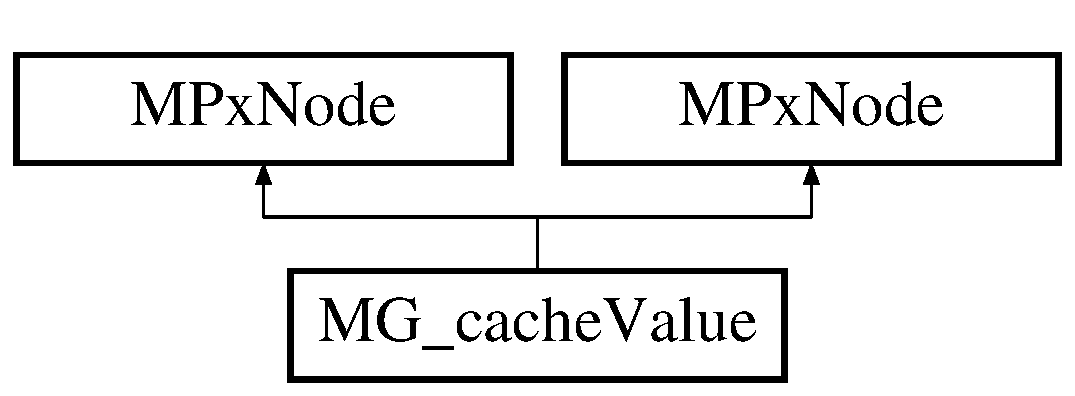
\includegraphics[height=2.000000cm]{class_m_g__cache_value}
\end{center}
\end{figure}
\subsection*{Public Member Functions}
\begin{DoxyCompactItemize}
\item 
\hypertarget{class_m_g__cache_value_a4af2a1a4fe6b3eafd7240561616bc89d}{virtual M\-Status {\bfseries compute} (const M\-Plug \&plug, M\-Data\-Block \&data\-Block)}\label{class_m_g__cache_value_a4af2a1a4fe6b3eafd7240561616bc89d}

\item 
\hypertarget{class_m_g__cache_value_a4af2a1a4fe6b3eafd7240561616bc89d}{virtual M\-Status {\bfseries compute} (const M\-Plug \&plug, M\-Data\-Block \&data\-Block)}\label{class_m_g__cache_value_a4af2a1a4fe6b3eafd7240561616bc89d}

\end{DoxyCompactItemize}
\subsection*{Static Public Member Functions}
\begin{DoxyCompactItemize}
\item 
\hypertarget{class_m_g__cache_value_af783feaf5d718ffda4fa0008beb18f21}{static void $\ast$ {\bfseries creator} ()}\label{class_m_g__cache_value_af783feaf5d718ffda4fa0008beb18f21}

\item 
\hypertarget{class_m_g__cache_value_af6f22c4b64bdc0c12061b120fad9db90}{static M\-Status {\bfseries initialize} ()}\label{class_m_g__cache_value_af6f22c4b64bdc0c12061b120fad9db90}

\item 
\hypertarget{class_m_g__cache_value_af783feaf5d718ffda4fa0008beb18f21}{static void $\ast$ {\bfseries creator} ()}\label{class_m_g__cache_value_af783feaf5d718ffda4fa0008beb18f21}

\item 
\hypertarget{class_m_g__cache_value_af6f22c4b64bdc0c12061b120fad9db90}{static M\-Status {\bfseries initialize} ()}\label{class_m_g__cache_value_af6f22c4b64bdc0c12061b120fad9db90}

\end{DoxyCompactItemize}
\subsection*{Static Public Attributes}
\begin{DoxyCompactItemize}
\item 
static M\-Type\-Id \hyperlink{class_m_g__cache_value_a4ce6876428ec0f2695f7004b69347c97}{type\-Id}
\item 
static M\-Object \hyperlink{class_m_g__cache_value_af24eadb6c01a5b74fe866b9ca17f0b01}{to\-Cache\-Value}
\item 
static M\-Object \hyperlink{class_m_g__cache_value_a2c30422a3a121f421f0c5e7fcb409848}{iteration\-Stored}
\item 
static M\-Object \hyperlink{class_m_g__cache_value_ab5b43d3f3f79cc1dbf14d2351fda4ce6}{out\-Value}
\item 
static M\-Object \hyperlink{class_m_g__cache_value_af41d3e0480acf043362b219ccab05313}{cache}
\item 
static M\-Object \hyperlink{class_m_g__cache_value_a07da37e093b60361fec58f19b35082cf}{past\-Iteration\-Out\-Index}
\end{DoxyCompactItemize}


\subsection{Detailed Description}
let s you cache a value 

\begin{DoxyAuthor}{Author}
Marco Giordano 
\end{DoxyAuthor}
\begin{DoxyDate}{Date}
10/1/2013 
\end{DoxyDate}
\begin{DoxyVersion}{Version}
latest version \-: V1 

changeload versions \-: \par
 V1 \-: \par

\begin{DoxyItemize}
\item initial release \par

\end{DoxyItemize}
\end{DoxyVersion}
node name \-: \hyperlink{class_m_g__cache_value}{M\-G\-\_\-cache\-Value}.

details \-: This node let s you cache a value This node let s you cache a value and then chose which iteration gives out as output

example create node \-: (M\-E\-L) create\-Node \hyperlink{class_m_g__cache_value}{M\-G\-\_\-cache\-Value}.

\begin{DoxyRefDesc}{Todo}
\item[\hyperlink{todo__todo000001}{Todo}]add baricentric coordinates computation mode\end{DoxyRefDesc}


\begin{DoxyAuthor}{Author}
Marco Giordano 
\end{DoxyAuthor}
\begin{DoxyDate}{Date}
10/1/2013 
\end{DoxyDate}
\begin{DoxyVersion}{Version}
latest version \-: V1 

changeload versions \-: \par
 V1 \-: \par

\begin{DoxyItemize}
\item initial release \par

\end{DoxyItemize}
\end{DoxyVersion}
node name \-: \hyperlink{class_m_g__cache_value}{M\-G\-\_\-cache\-Value}.

details \-: This node let s you cache a value This node let s you cache a value and then chose which iteration gives out as output

example create node \-: (M\-E\-L) create\-Node \hyperlink{class_m_g__cache_value}{M\-G\-\_\-cache\-Value}.

\begin{DoxyRefDesc}{Todo}
\item[\hyperlink{todo__todo000006}{Todo}]add baricentric coordinates computation mode\end{DoxyRefDesc}


\subsection{Member Data Documentation}
\hypertarget{class_m_g__cache_value_af41d3e0480acf043362b219ccab05313}{\index{M\-G\-\_\-cache\-Value@{M\-G\-\_\-cache\-Value}!cache@{cache}}
\index{cache@{cache}!MG_cacheValue@{M\-G\-\_\-cache\-Value}}
\subsubsection[{cache}]{\setlength{\rightskip}{0pt plus 5cm}static M\-Object M\-G\-\_\-cache\-Value\-::cache\hspace{0.3cm}{\ttfamily [static]}}}\label{class_m_g__cache_value_af41d3e0480acf043362b219ccab05313}
This is the attribute that holds the cache \hypertarget{class_m_g__cache_value_a2c30422a3a121f421f0c5e7fcb409848}{\index{M\-G\-\_\-cache\-Value@{M\-G\-\_\-cache\-Value}!iteration\-Stored@{iteration\-Stored}}
\index{iteration\-Stored@{iteration\-Stored}!MG_cacheValue@{M\-G\-\_\-cache\-Value}}
\subsubsection[{iteration\-Stored}]{\setlength{\rightskip}{0pt plus 5cm}static M\-Object M\-G\-\_\-cache\-Value\-::iteration\-Stored\hspace{0.3cm}{\ttfamily [static]}}}\label{class_m_g__cache_value_a2c30422a3a121f421f0c5e7fcb409848}
This attribute sets how many iteration will be stored in the node \hypertarget{class_m_g__cache_value_ab5b43d3f3f79cc1dbf14d2351fda4ce6}{\index{M\-G\-\_\-cache\-Value@{M\-G\-\_\-cache\-Value}!out\-Value@{out\-Value}}
\index{out\-Value@{out\-Value}!MG_cacheValue@{M\-G\-\_\-cache\-Value}}
\subsubsection[{out\-Value}]{\setlength{\rightskip}{0pt plus 5cm}static M\-Object M\-G\-\_\-cache\-Value\-::out\-Value\hspace{0.3cm}{\ttfamily [static]}}}\label{class_m_g__cache_value_ab5b43d3f3f79cc1dbf14d2351fda4ce6}
This attribute is the out value \hypertarget{class_m_g__cache_value_a07da37e093b60361fec58f19b35082cf}{\index{M\-G\-\_\-cache\-Value@{M\-G\-\_\-cache\-Value}!past\-Iteration\-Out\-Index@{past\-Iteration\-Out\-Index}}
\index{past\-Iteration\-Out\-Index@{past\-Iteration\-Out\-Index}!MG_cacheValue@{M\-G\-\_\-cache\-Value}}
\subsubsection[{past\-Iteration\-Out\-Index}]{\setlength{\rightskip}{0pt plus 5cm}static M\-Object M\-G\-\_\-cache\-Value\-::past\-Iteration\-Out\-Index\hspace{0.3cm}{\ttfamily [static]}}}\label{class_m_g__cache_value_a07da37e093b60361fec58f19b35082cf}
This attribute defines which past iteration index to show out , remember index 0 is present value , index 1 is the first past value and so on \hypertarget{class_m_g__cache_value_af24eadb6c01a5b74fe866b9ca17f0b01}{\index{M\-G\-\_\-cache\-Value@{M\-G\-\_\-cache\-Value}!to\-Cache\-Value@{to\-Cache\-Value}}
\index{to\-Cache\-Value@{to\-Cache\-Value}!MG_cacheValue@{M\-G\-\_\-cache\-Value}}
\subsubsection[{to\-Cache\-Value}]{\setlength{\rightskip}{0pt plus 5cm}static M\-Object M\-G\-\_\-cache\-Value\-::to\-Cache\-Value\hspace{0.3cm}{\ttfamily [static]}}}\label{class_m_g__cache_value_af24eadb6c01a5b74fe866b9ca17f0b01}
T\-His is the input value that is going to be cached \hypertarget{class_m_g__cache_value_a4ce6876428ec0f2695f7004b69347c97}{\index{M\-G\-\_\-cache\-Value@{M\-G\-\_\-cache\-Value}!type\-Id@{type\-Id}}
\index{type\-Id@{type\-Id}!MG_cacheValue@{M\-G\-\_\-cache\-Value}}
\subsubsection[{type\-Id}]{\setlength{\rightskip}{0pt plus 5cm}static M\-Type\-Id M\-G\-\_\-cache\-Value\-::type\-Id\hspace{0.3cm}{\ttfamily [static]}}}\label{class_m_g__cache_value_a4ce6876428ec0f2695f7004b69347c97}
The node id 

The documentation for this class was generated from the following files\-:\begin{DoxyCompactItemize}
\item 
C\-:/\-Users/giordi/\-Desktop/\-P\-R\-O\-G\-E\-T\-T\-I\-\_\-\-I\-N\-\_\-\-C\-O\-R\-S\-O/\-C/\-M\-G\-\_\-\-Tools/cpp/\-M\-G\-\_\-cache\-Value/src/M\-G\-\_\-cache\-Value.\-h\item 
C\-:/\-Users/giordi/\-Desktop/\-P\-R\-O\-G\-E\-T\-T\-I\-\_\-\-I\-N\-\_\-\-C\-O\-R\-S\-O/\-C/\-M\-G\-\_\-\-Tools/cpp/\-M\-G\-\_\-tools\-Lite/src/M\-G\-\_\-cache\-Value.\-h\end{DoxyCompactItemize}

\hypertarget{class_m_g__cross_product}{\section{M\-G\-\_\-cross\-Product Class Reference}
\label{class_m_g__cross_product}\index{M\-G\-\_\-cross\-Product@{M\-G\-\_\-cross\-Product}}
}


let s you perform cross product and related operations  




{\ttfamily \#include $<$M\-G\-\_\-cross\-Product.\-h$>$}

Inheritance diagram for M\-G\-\_\-cross\-Product\-:\begin{figure}[H]
\begin{center}
\leavevmode
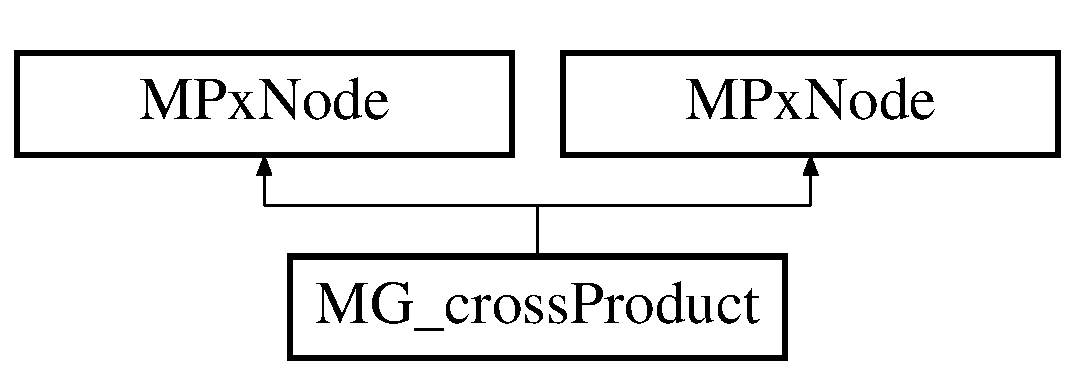
\includegraphics[height=2.000000cm]{class_m_g__cross_product}
\end{center}
\end{figure}
\subsection*{Public Member Functions}
\begin{DoxyCompactItemize}
\item 
\hypertarget{class_m_g__cross_product_a278dcb85153730af7f36eb05f887e230}{virtual M\-Status {\bfseries compute} (const M\-Plug \&plug, M\-Data\-Block \&data\-Block)}\label{class_m_g__cross_product_a278dcb85153730af7f36eb05f887e230}

\item 
\hypertarget{class_m_g__cross_product_a278dcb85153730af7f36eb05f887e230}{virtual M\-Status {\bfseries compute} (const M\-Plug \&plug, M\-Data\-Block \&data\-Block)}\label{class_m_g__cross_product_a278dcb85153730af7f36eb05f887e230}

\end{DoxyCompactItemize}
\subsection*{Static Public Member Functions}
\begin{DoxyCompactItemize}
\item 
\hypertarget{class_m_g__cross_product_a6c0c38d7c539ff59c3f91cb85bd1af16}{static void $\ast$ {\bfseries creator} ()}\label{class_m_g__cross_product_a6c0c38d7c539ff59c3f91cb85bd1af16}

\item 
\hypertarget{class_m_g__cross_product_a75e7dd903714ea50d1f21241077ee555}{static M\-Status {\bfseries initialize} ()}\label{class_m_g__cross_product_a75e7dd903714ea50d1f21241077ee555}

\item 
\hypertarget{class_m_g__cross_product_a6c0c38d7c539ff59c3f91cb85bd1af16}{static void $\ast$ {\bfseries creator} ()}\label{class_m_g__cross_product_a6c0c38d7c539ff59c3f91cb85bd1af16}

\item 
\hypertarget{class_m_g__cross_product_a75e7dd903714ea50d1f21241077ee555}{static M\-Status {\bfseries initialize} ()}\label{class_m_g__cross_product_a75e7dd903714ea50d1f21241077ee555}

\end{DoxyCompactItemize}
\subsection*{Static Public Attributes}
\begin{DoxyCompactItemize}
\item 
\hypertarget{class_m_g__cross_product_a168a1bd8516dcdd48b7b411690e4ace1}{static M\-Object {\bfseries vector1}}\label{class_m_g__cross_product_a168a1bd8516dcdd48b7b411690e4ace1}

\item 
\hypertarget{class_m_g__cross_product_a02537162bdc9d36081799eb510bf5e33}{static M\-Object {\bfseries vector2}}\label{class_m_g__cross_product_a02537162bdc9d36081799eb510bf5e33}

\item 
\hypertarget{class_m_g__cross_product_a90700f4d43108bdfba82432a76d8eda9}{static M\-Object {\bfseries normalize}}\label{class_m_g__cross_product_a90700f4d43108bdfba82432a76d8eda9}

\item 
\hypertarget{class_m_g__cross_product_adbedd1ca22359e0ef993e18b5fd7bb55}{static M\-Object {\bfseries cross\-Product\-A}}\label{class_m_g__cross_product_adbedd1ca22359e0ef993e18b5fd7bb55}

\item 
\hypertarget{class_m_g__cross_product_a89b59a4e0255cfdb96b3d235ff9cb0ef}{static M\-Object {\bfseries reverse}}\label{class_m_g__cross_product_a89b59a4e0255cfdb96b3d235ff9cb0ef}

\item 
\hypertarget{class_m_g__cross_product_ae04ffba8f459592e3ee0128a8bb36576}{static M\-Object {\bfseries parallelogram\-A}}\label{class_m_g__cross_product_ae04ffba8f459592e3ee0128a8bb36576}

\item 
\hypertarget{class_m_g__cross_product_ad12d96fd5106cddf312b04c468ef36f9}{static M\-Object {\bfseries triangle\-A}}\label{class_m_g__cross_product_ad12d96fd5106cddf312b04c468ef36f9}

\item 
\hypertarget{class_m_g__cross_product_a9947b42b254eb4c86f8d190a3652ceea}{static M\-Type\-Id {\bfseries type\-Id}}\label{class_m_g__cross_product_a9947b42b254eb4c86f8d190a3652ceea}

\end{DoxyCompactItemize}


\subsection{Detailed Description}
let s you perform cross product and related operations 

\begin{DoxyAuthor}{Author}
Marco Giordano 
\end{DoxyAuthor}
\begin{DoxyDate}{Date}
--/--/2011 
\end{DoxyDate}
\begin{DoxyVersion}{Version}
latest version \-: V1 

changeload versions \-: \par
 V1 \-: \par

\begin{DoxyItemize}
\item initial release \par

\end{DoxyItemize}
\end{DoxyVersion}
node name \-: \hyperlink{class_m_g__cross_product}{M\-G\-\_\-cross\-Product}.

details \-: This node let s you perform crost product and related operations This nodes needs as input two vectors and then in output you get several value and data you can use. Available output attribute \-:
\begin{DoxyItemize}
\item vector1 \-: first vector input
\item vector2 \-: second vector input
\item normalize \-: lets you normalize the crossed vector
\item reverse \-: lets you reverse the crossed vector
\item parallelogram area \-: this is the area of the paralleogram built with the two vectors
\item triangle area \-: this is the areao of the triangle built from the two vectors
\end{DoxyItemize}

example create node \-: (M\-E\-L) create\-Node \hyperlink{class_m_g__cross_product}{M\-G\-\_\-cross\-Product}. 

The documentation for this class was generated from the following files\-:\begin{DoxyCompactItemize}
\item 
C\-:/\-Users/giordi/\-Desktop/\-P\-R\-O\-G\-E\-T\-T\-I\-\_\-\-I\-N\-\_\-\-C\-O\-R\-S\-O/\-C/\-M\-G\-\_\-\-Tools/cpp/\-M\-G\-\_\-cross\-Product/src/M\-G\-\_\-cross\-Product.\-h\item 
C\-:/\-Users/giordi/\-Desktop/\-P\-R\-O\-G\-E\-T\-T\-I\-\_\-\-I\-N\-\_\-\-C\-O\-R\-S\-O/\-C/\-M\-G\-\_\-\-Tools/cpp/\-M\-G\-\_\-tools\-Lite/src/M\-G\-\_\-cross\-Product.\-h\end{DoxyCompactItemize}

\hypertarget{class_m_g__curve}{\section{M\-G\-\_\-curve Class Reference}
\label{class_m_g__curve}\index{M\-G\-\_\-curve@{M\-G\-\_\-curve}}
}


lets you generate a curve out of transform  




{\ttfamily \#include $<$M\-G\-\_\-curve.\-h$>$}

Inheritance diagram for M\-G\-\_\-curve\-:\begin{figure}[H]
\begin{center}
\leavevmode
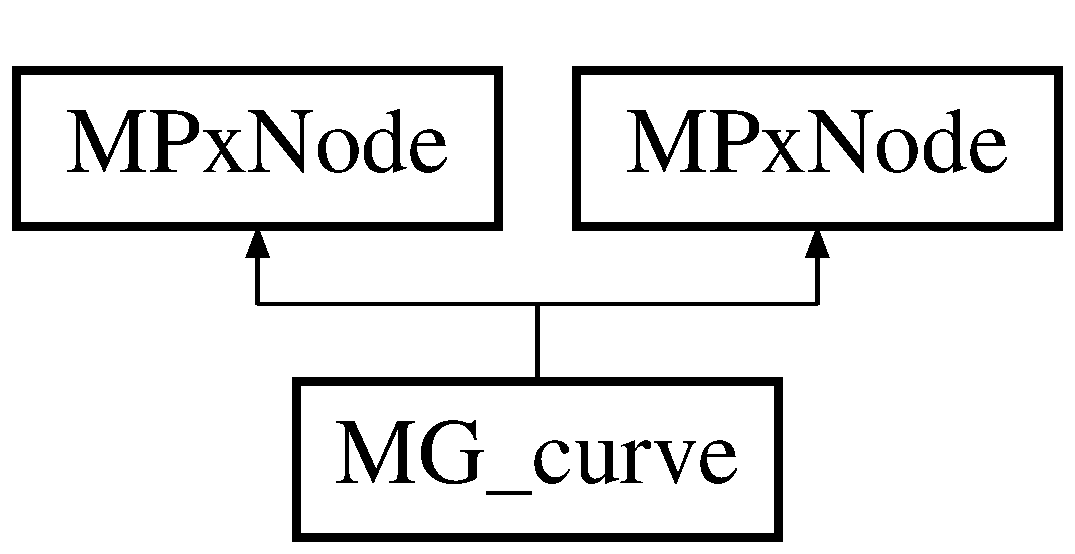
\includegraphics[height=2.000000cm]{class_m_g__curve}
\end{center}
\end{figure}
\subsection*{Public Member Functions}
\begin{DoxyCompactItemize}
\item 
\hypertarget{class_m_g__curve_aa9e2aace51476f58e756ab25b70c489a}{virtual M\-Status {\bfseries compute} (const M\-Plug \&plug, M\-Data\-Block \&data\-Block)}\label{class_m_g__curve_aa9e2aace51476f58e756ab25b70c489a}

\item 
\hypertarget{class_m_g__curve_aa9e2aace51476f58e756ab25b70c489a}{virtual M\-Status {\bfseries compute} (const M\-Plug \&plug, M\-Data\-Block \&data\-Block)}\label{class_m_g__curve_aa9e2aace51476f58e756ab25b70c489a}

\end{DoxyCompactItemize}
\subsection*{Static Public Member Functions}
\begin{DoxyCompactItemize}
\item 
\hypertarget{class_m_g__curve_a55d53bd06193f14a0dd1b987988bb5ef}{static void $\ast$ {\bfseries creator} ()}\label{class_m_g__curve_a55d53bd06193f14a0dd1b987988bb5ef}

\item 
\hypertarget{class_m_g__curve_ac628fa6a2f76d76986121ea3f1401bc3}{static M\-Status {\bfseries initialize} ()}\label{class_m_g__curve_ac628fa6a2f76d76986121ea3f1401bc3}

\item 
\hypertarget{class_m_g__curve_a55d53bd06193f14a0dd1b987988bb5ef}{static void $\ast$ {\bfseries creator} ()}\label{class_m_g__curve_a55d53bd06193f14a0dd1b987988bb5ef}

\item 
\hypertarget{class_m_g__curve_ac628fa6a2f76d76986121ea3f1401bc3}{static M\-Status {\bfseries initialize} ()}\label{class_m_g__curve_ac628fa6a2f76d76986121ea3f1401bc3}

\end{DoxyCompactItemize}
\subsection*{Static Public Attributes}
\begin{DoxyCompactItemize}
\item 
static M\-Object \hyperlink{class_m_g__curve_a81892d761eb59f6ae72dc5455e37de26}{input\-Matrix}
\item 
static M\-Object \hyperlink{class_m_g__curve_a2e9dc1c2f81ae96e443d7ce8db7ff668}{output}
\item 
static M\-Object \hyperlink{class_m_g__curve_a3330e534c2b2d2b7db3c621af0c4d6b2}{degree}
\item 
static M\-Object \hyperlink{class_m_g__curve_a03d8b8f59871792f08bc09ad64447354}{transform\-Matrix}
\item 
static M\-Type\-Id \hyperlink{class_m_g__curve_aaefd29164297e9889c41608b8b7f2542}{type\-Id}
\end{DoxyCompactItemize}


\subsection{Detailed Description}
lets you generate a curve out of transform 

\begin{DoxyAuthor}{Author}
Marco Giordano 
\end{DoxyAuthor}
\begin{DoxyDate}{Date}
11/13/2012 
\end{DoxyDate}
\begin{DoxyVersion}{Version}
latest version \-: V1 

changeload versions \-: \par
 V1 \-: \par

\begin{DoxyItemize}
\item initial release \par

\end{DoxyItemize}
\end{DoxyVersion}
node name \-: \hyperlink{class_m_g__curve}{M\-G\-\_\-curve}.

details \-: This node let you create a nurbs curve using an X number of transform as control\-Points. T\-He output of this node is not a simple float but a shape , so i suggest you to create a nurbs curve like a circle and then override the connection in the \char`\"{}create\char`\"{} attribute in the curve shape

example create node \-: (M\-E\-L) create\-Node \hyperlink{class_m_g__curve}{M\-G\-\_\-curve}. 

\subsection{Member Data Documentation}
\hypertarget{class_m_g__curve_a3330e534c2b2d2b7db3c621af0c4d6b2}{\index{M\-G\-\_\-curve@{M\-G\-\_\-curve}!degree@{degree}}
\index{degree@{degree}!MG_curve@{M\-G\-\_\-curve}}
\subsubsection[{degree}]{\setlength{\rightskip}{0pt plus 5cm}static M\-Object M\-G\-\_\-curve\-::degree\hspace{0.3cm}{\ttfamily [static]}}}\label{class_m_g__curve_a3330e534c2b2d2b7db3c621af0c4d6b2}
This is the degree we want to use for the curve \hypertarget{class_m_g__curve_a81892d761eb59f6ae72dc5455e37de26}{\index{M\-G\-\_\-curve@{M\-G\-\_\-curve}!input\-Matrix@{input\-Matrix}}
\index{input\-Matrix@{input\-Matrix}!MG_curve@{M\-G\-\_\-curve}}
\subsubsection[{input\-Matrix}]{\setlength{\rightskip}{0pt plus 5cm}static M\-Object M\-G\-\_\-curve\-::input\-Matrix\hspace{0.3cm}{\ttfamily [static]}}}\label{class_m_g__curve_a81892d761eb59f6ae72dc5455e37de26}
This is the attribute holding the input world matrix array \hypertarget{class_m_g__curve_a2e9dc1c2f81ae96e443d7ce8db7ff668}{\index{M\-G\-\_\-curve@{M\-G\-\_\-curve}!output@{output}}
\index{output@{output}!MG_curve@{M\-G\-\_\-curve}}
\subsubsection[{output}]{\setlength{\rightskip}{0pt plus 5cm}static M\-Object M\-G\-\_\-curve\-::output\hspace{0.3cm}{\ttfamily [static]}}}\label{class_m_g__curve_a2e9dc1c2f81ae96e443d7ce8db7ff668}
This is the output shape of the curve \hypertarget{class_m_g__curve_a03d8b8f59871792f08bc09ad64447354}{\index{M\-G\-\_\-curve@{M\-G\-\_\-curve}!transform\-Matrix@{transform\-Matrix}}
\index{transform\-Matrix@{transform\-Matrix}!MG_curve@{M\-G\-\_\-curve}}
\subsubsection[{transform\-Matrix}]{\setlength{\rightskip}{0pt plus 5cm}static M\-Object M\-G\-\_\-curve\-::transform\-Matrix\hspace{0.3cm}{\ttfamily [static]}}}\label{class_m_g__curve_a03d8b8f59871792f08bc09ad64447354}
Plug this value holds the transform world matrix of the curve , if you plug it in the node we will multipy the point for the inverse matrix so the curve wont be affected by its transform \hypertarget{class_m_g__curve_aaefd29164297e9889c41608b8b7f2542}{\index{M\-G\-\_\-curve@{M\-G\-\_\-curve}!type\-Id@{type\-Id}}
\index{type\-Id@{type\-Id}!MG_curve@{M\-G\-\_\-curve}}
\subsubsection[{type\-Id}]{\setlength{\rightskip}{0pt plus 5cm}static M\-Type\-Id M\-G\-\_\-curve\-::type\-Id\hspace{0.3cm}{\ttfamily [static]}}}\label{class_m_g__curve_aaefd29164297e9889c41608b8b7f2542}
The node id 

The documentation for this class was generated from the following files\-:\begin{DoxyCompactItemize}
\item 
C\-:/\-Users/giordi/\-Desktop/\-P\-R\-O\-G\-E\-T\-T\-I\-\_\-\-I\-N\-\_\-\-C\-O\-R\-S\-O/\-C/\-M\-G\-\_\-\-Tools/cpp/\-M\-G\-\_\-curve/src/M\-G\-\_\-curve.\-h\item 
C\-:/\-Users/giordi/\-Desktop/\-P\-R\-O\-G\-E\-T\-T\-I\-\_\-\-I\-N\-\_\-\-C\-O\-R\-S\-O/\-C/\-M\-G\-\_\-\-Tools/cpp/\-M\-G\-\_\-tools\-Lite/src/M\-G\-\_\-curve.\-h\end{DoxyCompactItemize}

\hypertarget{class_m_g__dot_product}{\section{M\-G\-\_\-dot\-Product Class Reference}
\label{class_m_g__dot_product}\index{M\-G\-\_\-dot\-Product@{M\-G\-\_\-dot\-Product}}
}


let s you perform dot product and related operations  




{\ttfamily \#include $<$M\-G\-\_\-dot\-Product.\-h$>$}

Inheritance diagram for M\-G\-\_\-dot\-Product\-:\begin{figure}[H]
\begin{center}
\leavevmode
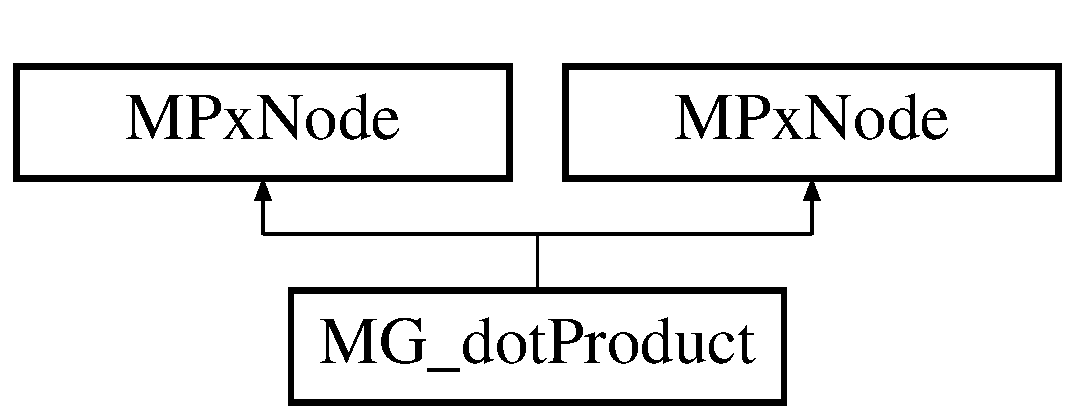
\includegraphics[height=2.000000cm]{class_m_g__dot_product}
\end{center}
\end{figure}
\subsection*{Public Member Functions}
\begin{DoxyCompactItemize}
\item 
\hypertarget{class_m_g__dot_product_a780fdeacba666efcead24e6668603ef8}{virtual M\-Status {\bfseries compute} (const M\-Plug \&plug, M\-Data\-Block \&data\-Block)}\label{class_m_g__dot_product_a780fdeacba666efcead24e6668603ef8}

\item 
\hypertarget{class_m_g__dot_product_a780fdeacba666efcead24e6668603ef8}{virtual M\-Status {\bfseries compute} (const M\-Plug \&plug, M\-Data\-Block \&data\-Block)}\label{class_m_g__dot_product_a780fdeacba666efcead24e6668603ef8}

\end{DoxyCompactItemize}
\subsection*{Static Public Member Functions}
\begin{DoxyCompactItemize}
\item 
\hypertarget{class_m_g__dot_product_ae28e061d3a46f47e453f0014c9388f79}{static void $\ast$ {\bfseries creator} ()}\label{class_m_g__dot_product_ae28e061d3a46f47e453f0014c9388f79}

\item 
\hypertarget{class_m_g__dot_product_ac1417ba72044571b4fbfb2f6407b7425}{static M\-Status {\bfseries initialize} ()}\label{class_m_g__dot_product_ac1417ba72044571b4fbfb2f6407b7425}

\item 
\hypertarget{class_m_g__dot_product_ae28e061d3a46f47e453f0014c9388f79}{static void $\ast$ {\bfseries creator} ()}\label{class_m_g__dot_product_ae28e061d3a46f47e453f0014c9388f79}

\item 
\hypertarget{class_m_g__dot_product_ac1417ba72044571b4fbfb2f6407b7425}{static M\-Status {\bfseries initialize} ()}\label{class_m_g__dot_product_ac1417ba72044571b4fbfb2f6407b7425}

\end{DoxyCompactItemize}
\subsection*{Static Public Attributes}
\begin{DoxyCompactItemize}
\item 
\hypertarget{class_m_g__dot_product_af502f55718b1cdc9c91daaa9b9d1df56}{static M\-Object {\bfseries vector1}}\label{class_m_g__dot_product_af502f55718b1cdc9c91daaa9b9d1df56}

\item 
\hypertarget{class_m_g__dot_product_a881bce730ab075c01577b70defe1d0e4}{static M\-Object {\bfseries vector2}}\label{class_m_g__dot_product_a881bce730ab075c01577b70defe1d0e4}

\item 
\hypertarget{class_m_g__dot_product_af400962818dc107b87ddf24b8fb85f7a}{static M\-Object {\bfseries dot\-Product\-A}}\label{class_m_g__dot_product_af400962818dc107b87ddf24b8fb85f7a}

\item 
\hypertarget{class_m_g__dot_product_aadac6df0d6b3ed24953710b6a6e1cba8}{static M\-Object {\bfseries normalize}}\label{class_m_g__dot_product_aadac6df0d6b3ed24953710b6a6e1cba8}

\item 
\hypertarget{class_m_g__dot_product_af1b6127de97b79b755c2d61899907d2a}{static M\-Object {\bfseries dot\-Product\-Max}}\label{class_m_g__dot_product_af1b6127de97b79b755c2d61899907d2a}

\item 
\hypertarget{class_m_g__dot_product_a675f64da0eedf32595e29860ff2c5626}{static M\-Object {\bfseries proj1on2}}\label{class_m_g__dot_product_a675f64da0eedf32595e29860ff2c5626}

\item 
\hypertarget{class_m_g__dot_product_aaf6b67d7596461619e1abdbaf0d0119e}{static M\-Object {\bfseries proj2on1}}\label{class_m_g__dot_product_aaf6b67d7596461619e1abdbaf0d0119e}

\item 
\hypertarget{class_m_g__dot_product_a1f5d8e8a523066d3fe0aa19204eb22ce}{static M\-Object {\bfseries angle\-In\-Between\-Attr}}\label{class_m_g__dot_product_a1f5d8e8a523066d3fe0aa19204eb22ce}

\item 
\hypertarget{class_m_g__dot_product_a48e882ea183c7e6b4a8bca37d5054350}{static M\-Object {\bfseries angle\-X}}\label{class_m_g__dot_product_a48e882ea183c7e6b4a8bca37d5054350}

\item 
\hypertarget{class_m_g__dot_product_ab6afd4f8254d8629b308f97bf06d177c}{static M\-Object {\bfseries angle\-Y}}\label{class_m_g__dot_product_ab6afd4f8254d8629b308f97bf06d177c}

\item 
\hypertarget{class_m_g__dot_product_ae292aa145b88ab47af49ee1d2dc69a1d}{static M\-Object {\bfseries angle\-Z}}\label{class_m_g__dot_product_ae292aa145b88ab47af49ee1d2dc69a1d}

\item 
\hypertarget{class_m_g__dot_product_a35d0dd4bc5d95356d98a86a136d33382}{static M\-Object {\bfseries proj\-Axis\-X}}\label{class_m_g__dot_product_a35d0dd4bc5d95356d98a86a136d33382}

\item 
\hypertarget{class_m_g__dot_product_a8da852cd1776f5937d1d9451296c2138}{static M\-Object {\bfseries proj\-Axis\-Xa}}\label{class_m_g__dot_product_a8da852cd1776f5937d1d9451296c2138}

\item 
\hypertarget{class_m_g__dot_product_a2946547c652010f265a1d6d76f0317f4}{static M\-Object {\bfseries proj\-Axis\-Xb}}\label{class_m_g__dot_product_a2946547c652010f265a1d6d76f0317f4}

\item 
\hypertarget{class_m_g__dot_product_a631919d46d5ae472d763a295be907d01}{static M\-Object {\bfseries proj\-Axis\-Xc}}\label{class_m_g__dot_product_a631919d46d5ae472d763a295be907d01}

\item 
\hypertarget{class_m_g__dot_product_a2eb03c42797ff7c42ef52fb6bb4dcecf}{static M\-Object {\bfseries proj\-Axis\-Y}}\label{class_m_g__dot_product_a2eb03c42797ff7c42ef52fb6bb4dcecf}

\item 
\hypertarget{class_m_g__dot_product_a1d2bc66cf065bb3d550fd2abb09f6655}{static M\-Object {\bfseries proj\-Axis\-Ya}}\label{class_m_g__dot_product_a1d2bc66cf065bb3d550fd2abb09f6655}

\item 
\hypertarget{class_m_g__dot_product_a1ad148e4b11ea6d87caae7f9373512b2}{static M\-Object {\bfseries proj\-Axis\-Yb}}\label{class_m_g__dot_product_a1ad148e4b11ea6d87caae7f9373512b2}

\item 
\hypertarget{class_m_g__dot_product_a3870fc4e3aac2cb695a07d906328e745}{static M\-Object {\bfseries proj\-Axis\-Yc}}\label{class_m_g__dot_product_a3870fc4e3aac2cb695a07d906328e745}

\item 
\hypertarget{class_m_g__dot_product_a5ad0e70c95ace16eb4f32ebad26cce5b}{static M\-Object {\bfseries proj\-Axis\-Z}}\label{class_m_g__dot_product_a5ad0e70c95ace16eb4f32ebad26cce5b}

\item 
\hypertarget{class_m_g__dot_product_a34204c917132a4a65b31ef6ea48b4e17}{static M\-Object {\bfseries proj\-Axis\-Za}}\label{class_m_g__dot_product_a34204c917132a4a65b31ef6ea48b4e17}

\item 
\hypertarget{class_m_g__dot_product_a59e3cb3a26e111df26c6703e50611855}{static M\-Object {\bfseries proj\-Axis\-Zb}}\label{class_m_g__dot_product_a59e3cb3a26e111df26c6703e50611855}

\item 
\hypertarget{class_m_g__dot_product_aeaa3f9c5ccaf5bac58df112e2fe0eb57}{static M\-Object {\bfseries proj\-Axis\-Zc}}\label{class_m_g__dot_product_aeaa3f9c5ccaf5bac58df112e2fe0eb57}

\item 
\hypertarget{class_m_g__dot_product_afed6410b30e30348b411f3407934a5d7}{static M\-Type\-Id {\bfseries type\-Id}}\label{class_m_g__dot_product_afed6410b30e30348b411f3407934a5d7}

\end{DoxyCompactItemize}


\subsection{Detailed Description}
let s you perform dot product and related operations 

\begin{DoxyAuthor}{Author}
Marco Giordano 
\end{DoxyAuthor}
\begin{DoxyDate}{Date}
--/--/2011 
\end{DoxyDate}
\begin{DoxyVersion}{Version}
latest version \-: V1 

changeload versions \-: \par
 V1 \-: \par

\begin{DoxyItemize}
\item initial release \par

\end{DoxyItemize}
\end{DoxyVersion}
node name \-: \hyperlink{class_m_g__dot_product}{M\-G\-\_\-dot\-Product}.

details \-: let s you perform dot product and related operations This nodes needs as input two vectors and then in output you get several value and data you can use. Available output attribute \-:
\begin{DoxyItemize}
\item angle\-Inbetween \-: the angle between the two vectors
\item angle X \-: the extracted angle x between the two vectors
\item angle Y \-: the extracted angle y between the two vectors
\item angle Z \-: the extracted angle z between the two vectors
\item dot\-Product \-: the dot product of the two vectors
\item dot\-Product\-Max\-Value \-: this attribute holds the max possible value for the dot product
\item normalize \-: this attribute lets you normalize the vectors and result of the operantions
\item projection\-V1on\-V2 \-: this is the value of the projection of V1 on V2
\item projection\-V2on\-V1 \-: this is the value of the projection of V2 on V1
\item x\-Axis\-Projection \-: default 1,0,0 change this value if you want project the vectors and angles in an not ortogonal world (advanced use only)
\item y\-Axis\-Projection \-: default 0,1,0 change this value if you want project the vectors and angles in an not ortogonal world (advanced use only)
\item z\-Axis\-Projection \-: default 0,0,1 change this value if you want project the vectors and angles in an not ortogonal world (advanced use only) example create node \-: (M\-E\-L) create\-Node \hyperlink{class_m_g__dot_product}{M\-G\-\_\-dot\-Product}. 
\end{DoxyItemize}

The documentation for this class was generated from the following files\-:\begin{DoxyCompactItemize}
\item 
C\-:/\-Users/giordi/\-Desktop/\-P\-R\-O\-G\-E\-T\-T\-I\-\_\-\-I\-N\-\_\-\-C\-O\-R\-S\-O/\-C/\-M\-G\-\_\-\-Tools/cpp/\-M\-G\-\_\-dot\-Product/src/M\-G\-\_\-dot\-Product.\-h\item 
C\-:/\-Users/giordi/\-Desktop/\-P\-R\-O\-G\-E\-T\-T\-I\-\_\-\-I\-N\-\_\-\-C\-O\-R\-S\-O/\-C/\-M\-G\-\_\-\-Tools/cpp/\-M\-G\-\_\-tools\-Lite/src/M\-G\-\_\-dot\-Product.\-h\end{DoxyCompactItemize}

\hypertarget{class_m_g__jiggle_vector}{\section{M\-G\-\_\-jiggle\-Vector Class Reference}
\label{class_m_g__jiggle_vector}\index{M\-G\-\_\-jiggle\-Vector@{M\-G\-\_\-jiggle\-Vector}}
}


Jiggle motion along vector direction.  




{\ttfamily \#include $<$M\-G\-\_\-jiggle\-Vector.\-h$>$}

Inheritance diagram for M\-G\-\_\-jiggle\-Vector\-:\begin{figure}[H]
\begin{center}
\leavevmode
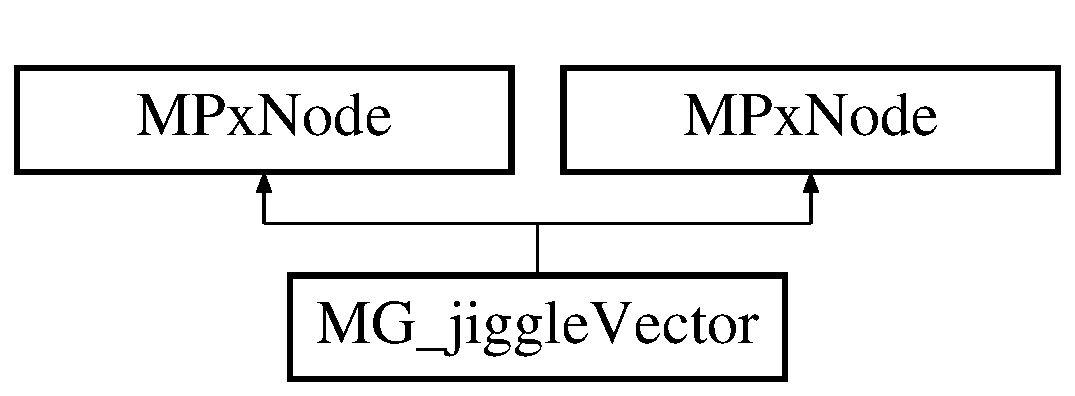
\includegraphics[height=2.000000cm]{class_m_g__jiggle_vector}
\end{center}
\end{figure}
\subsection*{Public Member Functions}
\begin{DoxyCompactItemize}
\item 
\hypertarget{class_m_g__jiggle_vector_a1e833e6b1d077c920a41e39f51b49333}{virtual M\-Status {\bfseries compute} (const M\-Plug \&plug, M\-Data\-Block \&data\-Block)}\label{class_m_g__jiggle_vector_a1e833e6b1d077c920a41e39f51b49333}

\item 
\hypertarget{class_m_g__jiggle_vector_a1e833e6b1d077c920a41e39f51b49333}{virtual M\-Status {\bfseries compute} (const M\-Plug \&plug, M\-Data\-Block \&data\-Block)}\label{class_m_g__jiggle_vector_a1e833e6b1d077c920a41e39f51b49333}

\end{DoxyCompactItemize}
\subsection*{Static Public Member Functions}
\begin{DoxyCompactItemize}
\item 
\hypertarget{class_m_g__jiggle_vector_a0121ffd8ea61b3fa769adae6d3ec46d5}{static void $\ast$ {\bfseries creator} ()}\label{class_m_g__jiggle_vector_a0121ffd8ea61b3fa769adae6d3ec46d5}

\item 
\hypertarget{class_m_g__jiggle_vector_afb29784790d236396b200b53e35623ba}{static M\-Status {\bfseries initialize} ()}\label{class_m_g__jiggle_vector_afb29784790d236396b200b53e35623ba}

\item 
\hypertarget{class_m_g__jiggle_vector_a0121ffd8ea61b3fa769adae6d3ec46d5}{static void $\ast$ {\bfseries creator} ()}\label{class_m_g__jiggle_vector_a0121ffd8ea61b3fa769adae6d3ec46d5}

\item 
\hypertarget{class_m_g__jiggle_vector_afb29784790d236396b200b53e35623ba}{static M\-Status {\bfseries initialize} ()}\label{class_m_g__jiggle_vector_afb29784790d236396b200b53e35623ba}

\end{DoxyCompactItemize}
\subsection*{Public Attributes}
\begin{DoxyCompactItemize}
\item 
\hypertarget{class_m_g__jiggle_vector_aa9f53afa76e98b44e7534522587acebd}{bool {\bfseries init}}\label{class_m_g__jiggle_vector_aa9f53afa76e98b44e7534522587acebd}

\item 
\hypertarget{class_m_g__jiggle_vector_aa7a47471e04d1f948fc3d70440284ac6}{double {\bfseries time\-Stored}}\label{class_m_g__jiggle_vector_aa7a47471e04d1f948fc3d70440284ac6}

\item 
\hypertarget{class_m_g__jiggle_vector_aef136bbc2480201c94748a9d5ebbf983}{M\-Point {\bfseries current\-Pos}}\label{class_m_g__jiggle_vector_aef136bbc2480201c94748a9d5ebbf983}

\item 
\hypertarget{class_m_g__jiggle_vector_a3192c684150e8801e1bde1fc36683244}{M\-Point {\bfseries previous\-Pos}}\label{class_m_g__jiggle_vector_a3192c684150e8801e1bde1fc36683244}

\end{DoxyCompactItemize}
\subsection*{Static Public Attributes}
\begin{DoxyCompactItemize}
\item 
static M\-Type\-Id \hyperlink{class_m_g__jiggle_vector_a5b2ebd5c51fb61ac246737c2871da7e7}{type\-Id}
\item 
static M\-Object \hyperlink{class_m_g__jiggle_vector_ada4c47f0dc60de027fe146bc1bf991f1}{output}
\item 
static M\-Object \hyperlink{class_m_g__jiggle_vector_a8165d97e3ab365d18a77af35ec9bd9d6}{output\-X}
\item 
static M\-Object \hyperlink{class_m_g__jiggle_vector_aa19e7d9b0b5f5f2066186a2106be7cb6}{output\-Y}
\item 
static M\-Object \hyperlink{class_m_g__jiggle_vector_a774f838b90e3bc2b823cffd43636ff43}{output\-Z}
\item 
static M\-Object \hyperlink{class_m_g__jiggle_vector_ab8ca0ac264688ec4588a06dc2de254d0}{damping}
\item 
static M\-Object \hyperlink{class_m_g__jiggle_vector_a9efc733e10f8b37b8ab5778c558d4668}{target\-Vector}
\item 
static M\-Object \hyperlink{class_m_g__jiggle_vector_aa16f19dc9c8b90569fdf39bfd6c9fd9e}{target\-Vector\-X}
\item 
static M\-Object \hyperlink{class_m_g__jiggle_vector_a075829bfac84e90a655e09dbf025e04f}{target\-Vector\-Y}
\item 
static M\-Object \hyperlink{class_m_g__jiggle_vector_aa1755e674e4bb7b580cf671eda0972b5}{target\-Vector\-Z}
\item 
static M\-Object \hyperlink{class_m_g__jiggle_vector_a41ea7a211dd0a1b21dd425aa39f3e358}{stiffness}
\item 
static M\-Object \hyperlink{class_m_g__jiggle_vector_a015c3c6cc0881e95de079788971e1f58}{time}
\item 
static M\-Object \hyperlink{class_m_g__jiggle_vector_a6e7dbbc9a06941e0b932b71e31050e32}{target\-Matrix}
\item 
static M\-Object \hyperlink{class_m_g__jiggle_vector_a680e0c72b6b00e9f828e441302753058}{use\-Start\-Frame}
\item 
static M\-Object \hyperlink{class_m_g__jiggle_vector_a2ffb1a14f9ead468f8dcf00df6c35652}{start\-Frame}
\item 
static M\-Object \hyperlink{class_m_g__jiggle_vector_a215dfaa566c1c46b1b248704298e588a}{reset}
\item 
static M\-Object \hyperlink{class_m_g__jiggle_vector_a8f397a47c080b1930f2637673ddd50b8}{clamp\-Max}
\item 
static M\-Object \hyperlink{class_m_g__jiggle_vector_a5f37c464cdbc951b5f71e1da2407facc}{clamp\-Min}
\item 
static M\-Object \hyperlink{class_m_g__jiggle_vector_aace586c7205919a5f2cfd3004e398fe1}{offset}
\item 
static M\-Object \hyperlink{class_m_g__jiggle_vector_a6731eddb749c12928566d0bcddb81983}{start\-Position}
\item 
static M\-Object \hyperlink{class_m_g__jiggle_vector_a14684897a82ddbe91f4a111ec0b0fbf5}{start\-Position\-X}
\item 
static M\-Object \hyperlink{class_m_g__jiggle_vector_a322050f97129dd0040871b3d9921e360}{start\-Position\-Y}
\item 
static M\-Object \hyperlink{class_m_g__jiggle_vector_a8934def35cd8c24f2af9c0f0edc03858}{start\-Position\-Z}
\item 
static M\-Object \hyperlink{class_m_g__jiggle_vector_a6fb6f77999b85dd0ed5ed38340215eb2}{clamp\-Range}
\item 
static M\-Object \hyperlink{class_m_g__jiggle_vector_ad81b7cebe25d1b1f6c4ef1d234233015}{use\-Local\-Output}
\item 
static M\-Object \hyperlink{class_m_g__jiggle_vector_aaf10913674da4674212e007b6175d140}{scale\-Fix}
\end{DoxyCompactItemize}


\subsection{Detailed Description}
Jiggle motion along vector direction. 

\begin{DoxyAuthor}{Author}
Marco Giordano 
\end{DoxyAuthor}
\begin{DoxyDate}{Date}
11/15/2012 
\end{DoxyDate}
\begin{DoxyVersion}{Version}
latest version \-: V1 

changeload versions \-: \par
 V1 \-: \par

\begin{DoxyItemize}
\item initial release \par

\end{DoxyItemize}
\end{DoxyVersion}
node name \-: \hyperlink{class_m_g__jiggle_vector}{M\-G\-\_\-jiggle\-Vector}.

details \-: Jiggle motion along vector direction This node needs the matrix of the target you want to generate the jiggle from and also needs the time node to be connected (usually this node is the time1). With this set you are good to go just connect the output to the translation of the target node. Use the parameters to se the nodes

example create node \-: (M\-E\-L) create\-Node \hyperlink{class_m_g__jiggle_vector}{M\-G\-\_\-jiggle\-Vector}. 

\subsection{Member Data Documentation}
\hypertarget{class_m_g__jiggle_vector_a8f397a47c080b1930f2637673ddd50b8}{\index{M\-G\-\_\-jiggle\-Vector@{M\-G\-\_\-jiggle\-Vector}!clamp\-Max@{clamp\-Max}}
\index{clamp\-Max@{clamp\-Max}!MG_jiggleVector@{M\-G\-\_\-jiggle\-Vector}}
\subsubsection[{clamp\-Max}]{\setlength{\rightskip}{0pt plus 5cm}static M\-Object M\-G\-\_\-jiggle\-Vector\-::clamp\-Max\hspace{0.3cm}{\ttfamily [static]}}}\label{class_m_g__jiggle_vector_a8f397a47c080b1930f2637673ddd50b8}
If clamp range is activated this attribute define the max of the range \hypertarget{class_m_g__jiggle_vector_a5f37c464cdbc951b5f71e1da2407facc}{\index{M\-G\-\_\-jiggle\-Vector@{M\-G\-\_\-jiggle\-Vector}!clamp\-Min@{clamp\-Min}}
\index{clamp\-Min@{clamp\-Min}!MG_jiggleVector@{M\-G\-\_\-jiggle\-Vector}}
\subsubsection[{clamp\-Min}]{\setlength{\rightskip}{0pt plus 5cm}static M\-Object M\-G\-\_\-jiggle\-Vector\-::clamp\-Min\hspace{0.3cm}{\ttfamily [static]}}}\label{class_m_g__jiggle_vector_a5f37c464cdbc951b5f71e1da2407facc}
If clamp range is activated this attribute define the min of the range \hypertarget{class_m_g__jiggle_vector_a6fb6f77999b85dd0ed5ed38340215eb2}{\index{M\-G\-\_\-jiggle\-Vector@{M\-G\-\_\-jiggle\-Vector}!clamp\-Range@{clamp\-Range}}
\index{clamp\-Range@{clamp\-Range}!MG_jiggleVector@{M\-G\-\_\-jiggle\-Vector}}
\subsubsection[{clamp\-Range}]{\setlength{\rightskip}{0pt plus 5cm}static M\-Object M\-G\-\_\-jiggle\-Vector\-::clamp\-Range\hspace{0.3cm}{\ttfamily [static]}}}\label{class_m_g__jiggle_vector_a6fb6f77999b85dd0ed5ed38340215eb2}
This attribute defines whether to clamp the jiggle or not \hypertarget{class_m_g__jiggle_vector_ab8ca0ac264688ec4588a06dc2de254d0}{\index{M\-G\-\_\-jiggle\-Vector@{M\-G\-\_\-jiggle\-Vector}!damping@{damping}}
\index{damping@{damping}!MG_jiggleVector@{M\-G\-\_\-jiggle\-Vector}}
\subsubsection[{damping}]{\setlength{\rightskip}{0pt plus 5cm}static M\-Object M\-G\-\_\-jiggle\-Vector\-::damping\hspace{0.3cm}{\ttfamily [static]}}}\label{class_m_g__jiggle_vector_ab8ca0ac264688ec4588a06dc2de254d0}
This attribute sets how much motion is getting lost \hypertarget{class_m_g__jiggle_vector_aace586c7205919a5f2cfd3004e398fe1}{\index{M\-G\-\_\-jiggle\-Vector@{M\-G\-\_\-jiggle\-Vector}!offset@{offset}}
\index{offset@{offset}!MG_jiggleVector@{M\-G\-\_\-jiggle\-Vector}}
\subsubsection[{offset}]{\setlength{\rightskip}{0pt plus 5cm}static M\-Object M\-G\-\_\-jiggle\-Vector\-::offset\hspace{0.3cm}{\ttfamily [static]}}}\label{class_m_g__jiggle_vector_aace586c7205919a5f2cfd3004e398fe1}
This attribute sets the amount of offset to apply to the jiggle \hypertarget{class_m_g__jiggle_vector_ada4c47f0dc60de027fe146bc1bf991f1}{\index{M\-G\-\_\-jiggle\-Vector@{M\-G\-\_\-jiggle\-Vector}!output@{output}}
\index{output@{output}!MG_jiggleVector@{M\-G\-\_\-jiggle\-Vector}}
\subsubsection[{output}]{\setlength{\rightskip}{0pt plus 5cm}static M\-Object M\-G\-\_\-jiggle\-Vector\-::output\hspace{0.3cm}{\ttfamily [static]}}}\label{class_m_g__jiggle_vector_ada4c47f0dc60de027fe146bc1bf991f1}
The output attribute \hypertarget{class_m_g__jiggle_vector_a8165d97e3ab365d18a77af35ec9bd9d6}{\index{M\-G\-\_\-jiggle\-Vector@{M\-G\-\_\-jiggle\-Vector}!output\-X@{output\-X}}
\index{output\-X@{output\-X}!MG_jiggleVector@{M\-G\-\_\-jiggle\-Vector}}
\subsubsection[{output\-X}]{\setlength{\rightskip}{0pt plus 5cm}static M\-Object M\-G\-\_\-jiggle\-Vector\-::output\-X\hspace{0.3cm}{\ttfamily [static]}}}\label{class_m_g__jiggle_vector_a8165d97e3ab365d18a77af35ec9bd9d6}
The output X for the compound attribute output \hypertarget{class_m_g__jiggle_vector_aa19e7d9b0b5f5f2066186a2106be7cb6}{\index{M\-G\-\_\-jiggle\-Vector@{M\-G\-\_\-jiggle\-Vector}!output\-Y@{output\-Y}}
\index{output\-Y@{output\-Y}!MG_jiggleVector@{M\-G\-\_\-jiggle\-Vector}}
\subsubsection[{output\-Y}]{\setlength{\rightskip}{0pt plus 5cm}static M\-Object M\-G\-\_\-jiggle\-Vector\-::output\-Y\hspace{0.3cm}{\ttfamily [static]}}}\label{class_m_g__jiggle_vector_aa19e7d9b0b5f5f2066186a2106be7cb6}
The output Y for the compound attribute output \hypertarget{class_m_g__jiggle_vector_a774f838b90e3bc2b823cffd43636ff43}{\index{M\-G\-\_\-jiggle\-Vector@{M\-G\-\_\-jiggle\-Vector}!output\-Z@{output\-Z}}
\index{output\-Z@{output\-Z}!MG_jiggleVector@{M\-G\-\_\-jiggle\-Vector}}
\subsubsection[{output\-Z}]{\setlength{\rightskip}{0pt plus 5cm}static M\-Object M\-G\-\_\-jiggle\-Vector\-::output\-Z\hspace{0.3cm}{\ttfamily [static]}}}\label{class_m_g__jiggle_vector_a774f838b90e3bc2b823cffd43636ff43}
The output Z for the compound attribute output \hypertarget{class_m_g__jiggle_vector_a215dfaa566c1c46b1b248704298e588a}{\index{M\-G\-\_\-jiggle\-Vector@{M\-G\-\_\-jiggle\-Vector}!reset@{reset}}
\index{reset@{reset}!MG_jiggleVector@{M\-G\-\_\-jiggle\-Vector}}
\subsubsection[{reset}]{\setlength{\rightskip}{0pt plus 5cm}static M\-Object M\-G\-\_\-jiggle\-Vector\-::reset\hspace{0.3cm}{\ttfamily [static]}}}\label{class_m_g__jiggle_vector_a215dfaa566c1c46b1b248704298e588a}
Reset the jiggle \hypertarget{class_m_g__jiggle_vector_aaf10913674da4674212e007b6175d140}{\index{M\-G\-\_\-jiggle\-Vector@{M\-G\-\_\-jiggle\-Vector}!scale\-Fix@{scale\-Fix}}
\index{scale\-Fix@{scale\-Fix}!MG_jiggleVector@{M\-G\-\_\-jiggle\-Vector}}
\subsubsection[{scale\-Fix}]{\setlength{\rightskip}{0pt plus 5cm}static M\-Object M\-G\-\_\-jiggle\-Vector\-::scale\-Fix\hspace{0.3cm}{\ttfamily [static]}}}\label{class_m_g__jiggle_vector_aaf10913674da4674212e007b6175d140}
If checked this attribute scales the jiggle based on the source scale \hypertarget{class_m_g__jiggle_vector_a2ffb1a14f9ead468f8dcf00df6c35652}{\index{M\-G\-\_\-jiggle\-Vector@{M\-G\-\_\-jiggle\-Vector}!start\-Frame@{start\-Frame}}
\index{start\-Frame@{start\-Frame}!MG_jiggleVector@{M\-G\-\_\-jiggle\-Vector}}
\subsubsection[{start\-Frame}]{\setlength{\rightskip}{0pt plus 5cm}static M\-Object M\-G\-\_\-jiggle\-Vector\-::start\-Frame\hspace{0.3cm}{\ttfamily [static]}}}\label{class_m_g__jiggle_vector_a2ffb1a14f9ead468f8dcf00df6c35652}
If use\-Start\-Frame attribute is checked then this attribute define which frame is the start frame \hypertarget{class_m_g__jiggle_vector_a6731eddb749c12928566d0bcddb81983}{\index{M\-G\-\_\-jiggle\-Vector@{M\-G\-\_\-jiggle\-Vector}!start\-Position@{start\-Position}}
\index{start\-Position@{start\-Position}!MG_jiggleVector@{M\-G\-\_\-jiggle\-Vector}}
\subsubsection[{start\-Position}]{\setlength{\rightskip}{0pt plus 5cm}static M\-Object M\-G\-\_\-jiggle\-Vector\-::start\-Position\hspace{0.3cm}{\ttfamily [static]}}}\label{class_m_g__jiggle_vector_a6731eddb749c12928566d0bcddb81983}
This is the start position for jiggle \hypertarget{class_m_g__jiggle_vector_a14684897a82ddbe91f4a111ec0b0fbf5}{\index{M\-G\-\_\-jiggle\-Vector@{M\-G\-\_\-jiggle\-Vector}!start\-Position\-X@{start\-Position\-X}}
\index{start\-Position\-X@{start\-Position\-X}!MG_jiggleVector@{M\-G\-\_\-jiggle\-Vector}}
\subsubsection[{start\-Position\-X}]{\setlength{\rightskip}{0pt plus 5cm}static M\-Object M\-G\-\_\-jiggle\-Vector\-::start\-Position\-X\hspace{0.3cm}{\ttfamily [static]}}}\label{class_m_g__jiggle_vector_a14684897a82ddbe91f4a111ec0b0fbf5}
This is X component of the start position for jiggle \hypertarget{class_m_g__jiggle_vector_a322050f97129dd0040871b3d9921e360}{\index{M\-G\-\_\-jiggle\-Vector@{M\-G\-\_\-jiggle\-Vector}!start\-Position\-Y@{start\-Position\-Y}}
\index{start\-Position\-Y@{start\-Position\-Y}!MG_jiggleVector@{M\-G\-\_\-jiggle\-Vector}}
\subsubsection[{start\-Position\-Y}]{\setlength{\rightskip}{0pt plus 5cm}static M\-Object M\-G\-\_\-jiggle\-Vector\-::start\-Position\-Y\hspace{0.3cm}{\ttfamily [static]}}}\label{class_m_g__jiggle_vector_a322050f97129dd0040871b3d9921e360}
This is Y component of the start position for jiggle \hypertarget{class_m_g__jiggle_vector_a8934def35cd8c24f2af9c0f0edc03858}{\index{M\-G\-\_\-jiggle\-Vector@{M\-G\-\_\-jiggle\-Vector}!start\-Position\-Z@{start\-Position\-Z}}
\index{start\-Position\-Z@{start\-Position\-Z}!MG_jiggleVector@{M\-G\-\_\-jiggle\-Vector}}
\subsubsection[{start\-Position\-Z}]{\setlength{\rightskip}{0pt plus 5cm}static M\-Object M\-G\-\_\-jiggle\-Vector\-::start\-Position\-Z\hspace{0.3cm}{\ttfamily [static]}}}\label{class_m_g__jiggle_vector_a8934def35cd8c24f2af9c0f0edc03858}
This is Z component of the start position for jiggle \hypertarget{class_m_g__jiggle_vector_a41ea7a211dd0a1b21dd425aa39f3e358}{\index{M\-G\-\_\-jiggle\-Vector@{M\-G\-\_\-jiggle\-Vector}!stiffness@{stiffness}}
\index{stiffness@{stiffness}!MG_jiggleVector@{M\-G\-\_\-jiggle\-Vector}}
\subsubsection[{stiffness}]{\setlength{\rightskip}{0pt plus 5cm}static M\-Object M\-G\-\_\-jiggle\-Vector\-::stiffness\hspace{0.3cm}{\ttfamily [static]}}}\label{class_m_g__jiggle_vector_a41ea7a211dd0a1b21dd425aa39f3e358}
This attribute sets how much attraction the source of the juggle apply \hypertarget{class_m_g__jiggle_vector_a6e7dbbc9a06941e0b932b71e31050e32}{\index{M\-G\-\_\-jiggle\-Vector@{M\-G\-\_\-jiggle\-Vector}!target\-Matrix@{target\-Matrix}}
\index{target\-Matrix@{target\-Matrix}!MG_jiggleVector@{M\-G\-\_\-jiggle\-Vector}}
\subsubsection[{target\-Matrix}]{\setlength{\rightskip}{0pt plus 5cm}static M\-Object M\-G\-\_\-jiggle\-Vector\-::target\-Matrix\hspace{0.3cm}{\ttfamily [static]}}}\label{class_m_g__jiggle_vector_a6e7dbbc9a06941e0b932b71e31050e32}
This is the source matrix from which the jiggle is generated from \hypertarget{class_m_g__jiggle_vector_a9efc733e10f8b37b8ab5778c558d4668}{\index{M\-G\-\_\-jiggle\-Vector@{M\-G\-\_\-jiggle\-Vector}!target\-Vector@{target\-Vector}}
\index{target\-Vector@{target\-Vector}!MG_jiggleVector@{M\-G\-\_\-jiggle\-Vector}}
\subsubsection[{target\-Vector}]{\setlength{\rightskip}{0pt plus 5cm}static M\-Object M\-G\-\_\-jiggle\-Vector\-::target\-Vector\hspace{0.3cm}{\ttfamily [static]}}}\label{class_m_g__jiggle_vector_a9efc733e10f8b37b8ab5778c558d4668}
This is the vector along you want to jiggle \hypertarget{class_m_g__jiggle_vector_aa16f19dc9c8b90569fdf39bfd6c9fd9e}{\index{M\-G\-\_\-jiggle\-Vector@{M\-G\-\_\-jiggle\-Vector}!target\-Vector\-X@{target\-Vector\-X}}
\index{target\-Vector\-X@{target\-Vector\-X}!MG_jiggleVector@{M\-G\-\_\-jiggle\-Vector}}
\subsubsection[{target\-Vector\-X}]{\setlength{\rightskip}{0pt plus 5cm}static M\-Object M\-G\-\_\-jiggle\-Vector\-::target\-Vector\-X\hspace{0.3cm}{\ttfamily [static]}}}\label{class_m_g__jiggle_vector_aa16f19dc9c8b90569fdf39bfd6c9fd9e}
The X component of the vector you want to perform the jiggle on \hypertarget{class_m_g__jiggle_vector_a075829bfac84e90a655e09dbf025e04f}{\index{M\-G\-\_\-jiggle\-Vector@{M\-G\-\_\-jiggle\-Vector}!target\-Vector\-Y@{target\-Vector\-Y}}
\index{target\-Vector\-Y@{target\-Vector\-Y}!MG_jiggleVector@{M\-G\-\_\-jiggle\-Vector}}
\subsubsection[{target\-Vector\-Y}]{\setlength{\rightskip}{0pt plus 5cm}static M\-Object M\-G\-\_\-jiggle\-Vector\-::target\-Vector\-Y\hspace{0.3cm}{\ttfamily [static]}}}\label{class_m_g__jiggle_vector_a075829bfac84e90a655e09dbf025e04f}
The Y component of the vector you want to perform the jiggle on \hypertarget{class_m_g__jiggle_vector_aa1755e674e4bb7b580cf671eda0972b5}{\index{M\-G\-\_\-jiggle\-Vector@{M\-G\-\_\-jiggle\-Vector}!target\-Vector\-Z@{target\-Vector\-Z}}
\index{target\-Vector\-Z@{target\-Vector\-Z}!MG_jiggleVector@{M\-G\-\_\-jiggle\-Vector}}
\subsubsection[{target\-Vector\-Z}]{\setlength{\rightskip}{0pt plus 5cm}static M\-Object M\-G\-\_\-jiggle\-Vector\-::target\-Vector\-Z\hspace{0.3cm}{\ttfamily [static]}}}\label{class_m_g__jiggle_vector_aa1755e674e4bb7b580cf671eda0972b5}
The Z component of the vector you want to perform the jiggle on \hypertarget{class_m_g__jiggle_vector_a015c3c6cc0881e95de079788971e1f58}{\index{M\-G\-\_\-jiggle\-Vector@{M\-G\-\_\-jiggle\-Vector}!time@{time}}
\index{time@{time}!MG_jiggleVector@{M\-G\-\_\-jiggle\-Vector}}
\subsubsection[{time}]{\setlength{\rightskip}{0pt plus 5cm}static M\-Object M\-G\-\_\-jiggle\-Vector\-::time\hspace{0.3cm}{\ttfamily [static]}}}\label{class_m_g__jiggle_vector_a015c3c6cc0881e95de079788971e1f58}
Connect to this attribute the maya time or another source of time \hypertarget{class_m_g__jiggle_vector_a5b2ebd5c51fb61ac246737c2871da7e7}{\index{M\-G\-\_\-jiggle\-Vector@{M\-G\-\_\-jiggle\-Vector}!type\-Id@{type\-Id}}
\index{type\-Id@{type\-Id}!MG_jiggleVector@{M\-G\-\_\-jiggle\-Vector}}
\subsubsection[{type\-Id}]{\setlength{\rightskip}{0pt plus 5cm}static M\-Type\-Id M\-G\-\_\-jiggle\-Vector\-::type\-Id\hspace{0.3cm}{\ttfamily [static]}}}\label{class_m_g__jiggle_vector_a5b2ebd5c51fb61ac246737c2871da7e7}
The node id \hypertarget{class_m_g__jiggle_vector_ad81b7cebe25d1b1f6c4ef1d234233015}{\index{M\-G\-\_\-jiggle\-Vector@{M\-G\-\_\-jiggle\-Vector}!use\-Local\-Output@{use\-Local\-Output}}
\index{use\-Local\-Output@{use\-Local\-Output}!MG_jiggleVector@{M\-G\-\_\-jiggle\-Vector}}
\subsubsection[{use\-Local\-Output}]{\setlength{\rightskip}{0pt plus 5cm}static M\-Object M\-G\-\_\-jiggle\-Vector\-::use\-Local\-Output\hspace{0.3cm}{\ttfamily [static]}}}\label{class_m_g__jiggle_vector_ad81b7cebe25d1b1f6c4ef1d234233015}
If the attribute is checked the jiggle will be local to the source of the jiggle \hypertarget{class_m_g__jiggle_vector_a680e0c72b6b00e9f828e441302753058}{\index{M\-G\-\_\-jiggle\-Vector@{M\-G\-\_\-jiggle\-Vector}!use\-Start\-Frame@{use\-Start\-Frame}}
\index{use\-Start\-Frame@{use\-Start\-Frame}!MG_jiggleVector@{M\-G\-\_\-jiggle\-Vector}}
\subsubsection[{use\-Start\-Frame}]{\setlength{\rightskip}{0pt plus 5cm}static M\-Object M\-G\-\_\-jiggle\-Vector\-::use\-Start\-Frame\hspace{0.3cm}{\ttfamily [static]}}}\label{class_m_g__jiggle_vector_a680e0c72b6b00e9f828e441302753058}
This attribute define if to use or not the start frame to reset the simulation 

The documentation for this class was generated from the following files\-:\begin{DoxyCompactItemize}
\item 
C\-:/\-Users/giordi/\-Desktop/\-P\-R\-O\-G\-E\-T\-T\-I\-\_\-\-I\-N\-\_\-\-C\-O\-R\-S\-O/\-C/\-M\-G\-\_\-\-Tools/cpp/\-M\-G\-\_\-jiggle\-Vector/src/M\-G\-\_\-jiggle\-Vector.\-h\item 
C\-:/\-Users/giordi/\-Desktop/\-P\-R\-O\-G\-E\-T\-T\-I\-\_\-\-I\-N\-\_\-\-C\-O\-R\-S\-O/\-C/\-M\-G\-\_\-\-Tools/cpp/\-M\-G\-\_\-tools\-Lite/src/M\-G\-\_\-jiggle\-Vector.\-h\end{DoxyCompactItemize}

\hypertarget{class_m_g__nurbs_rivet}{\section{M\-G\-\_\-nurbs\-Rivet Class Reference}
\label{class_m_g__nurbs_rivet}\index{M\-G\-\_\-nurbs\-Rivet@{M\-G\-\_\-nurbs\-Rivet}}
}


lets you constraint an object on a nurbs surface  




{\ttfamily \#include $<$M\-G\-\_\-nurbs\-Rivet.\-h$>$}

Inheritance diagram for M\-G\-\_\-nurbs\-Rivet\-:\begin{figure}[H]
\begin{center}
\leavevmode
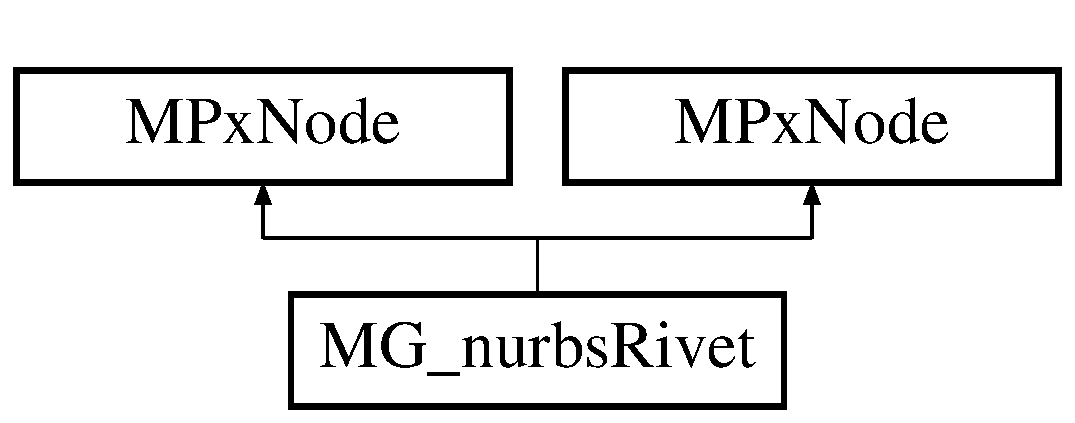
\includegraphics[height=2.000000cm]{class_m_g__nurbs_rivet}
\end{center}
\end{figure}
\subsection*{Public Member Functions}
\begin{DoxyCompactItemize}
\item 
\hypertarget{class_m_g__nurbs_rivet_af5e330b27dcb22d5baeb8787b0c36f6b}{virtual M\-Status {\bfseries compute} (const M\-Plug \&plug, M\-Data\-Block \&data\-Block)}\label{class_m_g__nurbs_rivet_af5e330b27dcb22d5baeb8787b0c36f6b}

\item 
\hypertarget{class_m_g__nurbs_rivet_af5e330b27dcb22d5baeb8787b0c36f6b}{virtual M\-Status {\bfseries compute} (const M\-Plug \&plug, M\-Data\-Block \&data\-Block)}\label{class_m_g__nurbs_rivet_af5e330b27dcb22d5baeb8787b0c36f6b}

\end{DoxyCompactItemize}
\subsection*{Static Public Member Functions}
\begin{DoxyCompactItemize}
\item 
\hypertarget{class_m_g__nurbs_rivet_a111738eae2e3af58b2a5ccb12da875e2}{static void $\ast$ {\bfseries creator} ()}\label{class_m_g__nurbs_rivet_a111738eae2e3af58b2a5ccb12da875e2}

\item 
\hypertarget{class_m_g__nurbs_rivet_a7e38c954eb834b9af8f3e5ac702af08a}{static M\-Status {\bfseries initialize} ()}\label{class_m_g__nurbs_rivet_a7e38c954eb834b9af8f3e5ac702af08a}

\item 
\hypertarget{class_m_g__nurbs_rivet_a111738eae2e3af58b2a5ccb12da875e2}{static void $\ast$ {\bfseries creator} ()}\label{class_m_g__nurbs_rivet_a111738eae2e3af58b2a5ccb12da875e2}

\item 
\hypertarget{class_m_g__nurbs_rivet_a7e38c954eb834b9af8f3e5ac702af08a}{static M\-Status {\bfseries initialize} ()}\label{class_m_g__nurbs_rivet_a7e38c954eb834b9af8f3e5ac702af08a}

\end{DoxyCompactItemize}
\subsection*{Static Public Attributes}
\begin{DoxyCompactItemize}
\item 
static M\-Object \hyperlink{class_m_g__nurbs_rivet_a560023fd0f07e418f27f5a2fff70981c}{input\-Nurb\-Surface}
\item 
static M\-Object \hyperlink{class_m_g__nurbs_rivet_a29e50ce621268c3947f456f3e43bfa25}{input\-Point}
\item 
static M\-Object \hyperlink{class_m_g__nurbs_rivet_a7aeccbeeb51f51b5bef973f01103e6b9}{recompute}
\item 
static M\-Object \hyperlink{class_m_g__nurbs_rivet_ac3d5177a9758f3b3ad1b61cad032229e}{output}
\item 
static M\-Object \hyperlink{class_m_g__nurbs_rivet_a2531bc3b5ef7d7585fcf8a3b3435590e}{u\-Value}
\item 
static M\-Object \hyperlink{class_m_g__nurbs_rivet_a3ed59e29adcdbf204f407f08fe3b16b5}{v\-Value}
\item 
static M\-Object \hyperlink{class_m_g__nurbs_rivet_a446ab71986b82fe1e09210e5f467e010}{output\-Rotate}
\item 
static M\-Object \hyperlink{class_m_g__nurbs_rivet_a5dc9d6a6ed4f7e24425c3f25f934eead}{output\-Matrix}
\item 
static M\-Object \hyperlink{class_m_g__nurbs_rivet_a540b3de13a7788eec9d1c08973bb1515}{offset\-Matrix}
\item 
static M\-Object \hyperlink{class_m_g__nurbs_rivet_a5c09cb3fe1b1eb73e8f75176b8e7b723}{input\-Point\-X}
\item 
static M\-Object \hyperlink{class_m_g__nurbs_rivet_a9d55b7bdff71504f9531f8924cfc7d10}{input\-Point\-Y}
\item 
static M\-Object \hyperlink{class_m_g__nurbs_rivet_acd26e9adfc47fe51b82fe0f6c8ae9bb3}{input\-Point\-Z}
\item 
static M\-Object \hyperlink{class_m_g__nurbs_rivet_a4166483abd2b8b57483d81dbc97f3de5}{output\-X}
\item 
static M\-Object \hyperlink{class_m_g__nurbs_rivet_a9dacbb8116714802ee9eb28176a1e38c}{output\-Y}
\item 
static M\-Object \hyperlink{class_m_g__nurbs_rivet_a923a0bc4a7e64e2a6179e7d55cffd2a9}{output\-Z}
\item 
static M\-Object \hyperlink{class_m_g__nurbs_rivet_a55491d93e5402c09f4463e8729a83c57}{output\-Rotate\-X}
\item 
static M\-Object \hyperlink{class_m_g__nurbs_rivet_a36757fb01097b3063e8ab7e09d33b104}{output\-Rotate\-Y}
\item 
static M\-Object \hyperlink{class_m_g__nurbs_rivet_aa561c384be7c4fc5634436c491af7aef}{output\-Rotate\-Z}
\item 
static M\-Type\-Id \hyperlink{class_m_g__nurbs_rivet_a0d32f63265a10d14a34eb6a6e3c8a355}{type\-Id}
\end{DoxyCompactItemize}


\subsection{Detailed Description}
lets you constraint an object on a nurbs surface 

\begin{DoxyAuthor}{Author}
Marco Giordano 
\end{DoxyAuthor}
\begin{DoxyVersion}{Version}
latest version \-: V2 

changeload versions \-: \par
 V1 \-: \par

\begin{DoxyItemize}
\item initial release \par
 
\end{DoxyItemize}

V2 \-:
\begin{DoxyItemize}
\item removed dependencie from vec\-Math.\-h (custom sloppy header)
\item cleaned code and made more efficient
\item added offset matrix
\end{DoxyItemize}
\end{DoxyVersion}
node name \-: \hyperlink{class_m_g__nurbs_rivet}{M\-G\-\_\-nurbs\-Rivet}.

details \-: This node let you constraint an object on a nurb surface This node needs as input an input point, the input point is the point from where the closest point on the nurbs will be calculated in order to place the rivet. An input nurbs surface has to be provided , just connect the \char`\"{}world\-Space\char`\"{} attribute from the shape of the wanted nurbs curve. If you want to keep an offset from the calculated rivet you can set the offset matrix in the node , this has to be calculate , I might provide a script for that in the feature. Once your happy with the rivet position you can uncheck the recompute attribute , in this way the closest point on surface wont be recomputed anymore , keep it on if you want to animate the i input point and slide the rivet on the surface

example create node \-: (M\-E\-L) create\-Node \hyperlink{class_m_g__nurbs_rivet}{M\-G\-\_\-nurbs\-Rivet}. 

\subsection{Member Data Documentation}
\hypertarget{class_m_g__nurbs_rivet_a560023fd0f07e418f27f5a2fff70981c}{\index{M\-G\-\_\-nurbs\-Rivet@{M\-G\-\_\-nurbs\-Rivet}!input\-Nurb\-Surface@{input\-Nurb\-Surface}}
\index{input\-Nurb\-Surface@{input\-Nurb\-Surface}!MG_nurbsRivet@{M\-G\-\_\-nurbs\-Rivet}}
\subsubsection[{input\-Nurb\-Surface}]{\setlength{\rightskip}{0pt plus 5cm}static M\-Object M\-G\-\_\-nurbs\-Rivet\-::input\-Nurb\-Surface\hspace{0.3cm}{\ttfamily [static]}}}\label{class_m_g__nurbs_rivet_a560023fd0f07e418f27f5a2fff70981c}
Connect to this input the shape of the nurbs\-Surface on which the rivet will stay on \hypertarget{class_m_g__nurbs_rivet_a29e50ce621268c3947f456f3e43bfa25}{\index{M\-G\-\_\-nurbs\-Rivet@{M\-G\-\_\-nurbs\-Rivet}!input\-Point@{input\-Point}}
\index{input\-Point@{input\-Point}!MG_nurbsRivet@{M\-G\-\_\-nurbs\-Rivet}}
\subsubsection[{input\-Point}]{\setlength{\rightskip}{0pt plus 5cm}static M\-Object M\-G\-\_\-nurbs\-Rivet\-::input\-Point\hspace{0.3cm}{\ttfamily [static]}}}\label{class_m_g__nurbs_rivet_a29e50ce621268c3947f456f3e43bfa25}
This is the initial position for the target object \hypertarget{class_m_g__nurbs_rivet_a5c09cb3fe1b1eb73e8f75176b8e7b723}{\index{M\-G\-\_\-nurbs\-Rivet@{M\-G\-\_\-nurbs\-Rivet}!input\-Point\-X@{input\-Point\-X}}
\index{input\-Point\-X@{input\-Point\-X}!MG_nurbsRivet@{M\-G\-\_\-nurbs\-Rivet}}
\subsubsection[{input\-Point\-X}]{\setlength{\rightskip}{0pt plus 5cm}static M\-Object M\-G\-\_\-nurbs\-Rivet\-::input\-Point\-X\hspace{0.3cm}{\ttfamily [static]}}}\label{class_m_g__nurbs_rivet_a5c09cb3fe1b1eb73e8f75176b8e7b723}
The input X for the compound attribute input\-Point \hypertarget{class_m_g__nurbs_rivet_a9d55b7bdff71504f9531f8924cfc7d10}{\index{M\-G\-\_\-nurbs\-Rivet@{M\-G\-\_\-nurbs\-Rivet}!input\-Point\-Y@{input\-Point\-Y}}
\index{input\-Point\-Y@{input\-Point\-Y}!MG_nurbsRivet@{M\-G\-\_\-nurbs\-Rivet}}
\subsubsection[{input\-Point\-Y}]{\setlength{\rightskip}{0pt plus 5cm}static M\-Object M\-G\-\_\-nurbs\-Rivet\-::input\-Point\-Y\hspace{0.3cm}{\ttfamily [static]}}}\label{class_m_g__nurbs_rivet_a9d55b7bdff71504f9531f8924cfc7d10}
The input Y for the compound attribute input\-Point \hypertarget{class_m_g__nurbs_rivet_acd26e9adfc47fe51b82fe0f6c8ae9bb3}{\index{M\-G\-\_\-nurbs\-Rivet@{M\-G\-\_\-nurbs\-Rivet}!input\-Point\-Z@{input\-Point\-Z}}
\index{input\-Point\-Z@{input\-Point\-Z}!MG_nurbsRivet@{M\-G\-\_\-nurbs\-Rivet}}
\subsubsection[{input\-Point\-Z}]{\setlength{\rightskip}{0pt plus 5cm}static M\-Object M\-G\-\_\-nurbs\-Rivet\-::input\-Point\-Z\hspace{0.3cm}{\ttfamily [static]}}}\label{class_m_g__nurbs_rivet_acd26e9adfc47fe51b82fe0f6c8ae9bb3}
The input Z for the compound attribute input\-Point \hypertarget{class_m_g__nurbs_rivet_a540b3de13a7788eec9d1c08973bb1515}{\index{M\-G\-\_\-nurbs\-Rivet@{M\-G\-\_\-nurbs\-Rivet}!offset\-Matrix@{offset\-Matrix}}
\index{offset\-Matrix@{offset\-Matrix}!MG_nurbsRivet@{M\-G\-\_\-nurbs\-Rivet}}
\subsubsection[{offset\-Matrix}]{\setlength{\rightskip}{0pt plus 5cm}static M\-Object M\-G\-\_\-nurbs\-Rivet\-::offset\-Matrix\hspace{0.3cm}{\ttfamily [static]}}}\label{class_m_g__nurbs_rivet_a540b3de13a7788eec9d1c08973bb1515}
This attribute holds the offset matrix from the rivet to the target that is going to be driven by the rivet \hypertarget{class_m_g__nurbs_rivet_ac3d5177a9758f3b3ad1b61cad032229e}{\index{M\-G\-\_\-nurbs\-Rivet@{M\-G\-\_\-nurbs\-Rivet}!output@{output}}
\index{output@{output}!MG_nurbsRivet@{M\-G\-\_\-nurbs\-Rivet}}
\subsubsection[{output}]{\setlength{\rightskip}{0pt plus 5cm}static M\-Object M\-G\-\_\-nurbs\-Rivet\-::output\hspace{0.3cm}{\ttfamily [static]}}}\label{class_m_g__nurbs_rivet_ac3d5177a9758f3b3ad1b61cad032229e}
The output translate attribute \hypertarget{class_m_g__nurbs_rivet_a5dc9d6a6ed4f7e24425c3f25f934eead}{\index{M\-G\-\_\-nurbs\-Rivet@{M\-G\-\_\-nurbs\-Rivet}!output\-Matrix@{output\-Matrix}}
\index{output\-Matrix@{output\-Matrix}!MG_nurbsRivet@{M\-G\-\_\-nurbs\-Rivet}}
\subsubsection[{output\-Matrix}]{\setlength{\rightskip}{0pt plus 5cm}static M\-Object M\-G\-\_\-nurbs\-Rivet\-::output\-Matrix\hspace{0.3cm}{\ttfamily [static]}}}\label{class_m_g__nurbs_rivet_a5dc9d6a6ed4f7e24425c3f25f934eead}
The output matrix attribute \hypertarget{class_m_g__nurbs_rivet_a446ab71986b82fe1e09210e5f467e010}{\index{M\-G\-\_\-nurbs\-Rivet@{M\-G\-\_\-nurbs\-Rivet}!output\-Rotate@{output\-Rotate}}
\index{output\-Rotate@{output\-Rotate}!MG_nurbsRivet@{M\-G\-\_\-nurbs\-Rivet}}
\subsubsection[{output\-Rotate}]{\setlength{\rightskip}{0pt plus 5cm}static M\-Object M\-G\-\_\-nurbs\-Rivet\-::output\-Rotate\hspace{0.3cm}{\ttfamily [static]}}}\label{class_m_g__nurbs_rivet_a446ab71986b82fe1e09210e5f467e010}
The output rotate attribute \hypertarget{class_m_g__nurbs_rivet_a55491d93e5402c09f4463e8729a83c57}{\index{M\-G\-\_\-nurbs\-Rivet@{M\-G\-\_\-nurbs\-Rivet}!output\-Rotate\-X@{output\-Rotate\-X}}
\index{output\-Rotate\-X@{output\-Rotate\-X}!MG_nurbsRivet@{M\-G\-\_\-nurbs\-Rivet}}
\subsubsection[{output\-Rotate\-X}]{\setlength{\rightskip}{0pt plus 5cm}static M\-Object M\-G\-\_\-nurbs\-Rivet\-::output\-Rotate\-X\hspace{0.3cm}{\ttfamily [static]}}}\label{class_m_g__nurbs_rivet_a55491d93e5402c09f4463e8729a83c57}
The output X for the compound attribute output\-Rotate \hypertarget{class_m_g__nurbs_rivet_a36757fb01097b3063e8ab7e09d33b104}{\index{M\-G\-\_\-nurbs\-Rivet@{M\-G\-\_\-nurbs\-Rivet}!output\-Rotate\-Y@{output\-Rotate\-Y}}
\index{output\-Rotate\-Y@{output\-Rotate\-Y}!MG_nurbsRivet@{M\-G\-\_\-nurbs\-Rivet}}
\subsubsection[{output\-Rotate\-Y}]{\setlength{\rightskip}{0pt plus 5cm}static M\-Object M\-G\-\_\-nurbs\-Rivet\-::output\-Rotate\-Y\hspace{0.3cm}{\ttfamily [static]}}}\label{class_m_g__nurbs_rivet_a36757fb01097b3063e8ab7e09d33b104}
The output Y for the compound attribute output\-Rotate \hypertarget{class_m_g__nurbs_rivet_aa561c384be7c4fc5634436c491af7aef}{\index{M\-G\-\_\-nurbs\-Rivet@{M\-G\-\_\-nurbs\-Rivet}!output\-Rotate\-Z@{output\-Rotate\-Z}}
\index{output\-Rotate\-Z@{output\-Rotate\-Z}!MG_nurbsRivet@{M\-G\-\_\-nurbs\-Rivet}}
\subsubsection[{output\-Rotate\-Z}]{\setlength{\rightskip}{0pt plus 5cm}static M\-Object M\-G\-\_\-nurbs\-Rivet\-::output\-Rotate\-Z\hspace{0.3cm}{\ttfamily [static]}}}\label{class_m_g__nurbs_rivet_aa561c384be7c4fc5634436c491af7aef}
The output Z for the compound attribute output\-Rotate \hypertarget{class_m_g__nurbs_rivet_a4166483abd2b8b57483d81dbc97f3de5}{\index{M\-G\-\_\-nurbs\-Rivet@{M\-G\-\_\-nurbs\-Rivet}!output\-X@{output\-X}}
\index{output\-X@{output\-X}!MG_nurbsRivet@{M\-G\-\_\-nurbs\-Rivet}}
\subsubsection[{output\-X}]{\setlength{\rightskip}{0pt plus 5cm}static M\-Object M\-G\-\_\-nurbs\-Rivet\-::output\-X\hspace{0.3cm}{\ttfamily [static]}}}\label{class_m_g__nurbs_rivet_a4166483abd2b8b57483d81dbc97f3de5}
The output X for the compound attribute output \hypertarget{class_m_g__nurbs_rivet_a9dacbb8116714802ee9eb28176a1e38c}{\index{M\-G\-\_\-nurbs\-Rivet@{M\-G\-\_\-nurbs\-Rivet}!output\-Y@{output\-Y}}
\index{output\-Y@{output\-Y}!MG_nurbsRivet@{M\-G\-\_\-nurbs\-Rivet}}
\subsubsection[{output\-Y}]{\setlength{\rightskip}{0pt plus 5cm}static M\-Object M\-G\-\_\-nurbs\-Rivet\-::output\-Y\hspace{0.3cm}{\ttfamily [static]}}}\label{class_m_g__nurbs_rivet_a9dacbb8116714802ee9eb28176a1e38c}
The output Y for the compound attribute output \hypertarget{class_m_g__nurbs_rivet_a923a0bc4a7e64e2a6179e7d55cffd2a9}{\index{M\-G\-\_\-nurbs\-Rivet@{M\-G\-\_\-nurbs\-Rivet}!output\-Z@{output\-Z}}
\index{output\-Z@{output\-Z}!MG_nurbsRivet@{M\-G\-\_\-nurbs\-Rivet}}
\subsubsection[{output\-Z}]{\setlength{\rightskip}{0pt plus 5cm}static M\-Object M\-G\-\_\-nurbs\-Rivet\-::output\-Z\hspace{0.3cm}{\ttfamily [static]}}}\label{class_m_g__nurbs_rivet_a923a0bc4a7e64e2a6179e7d55cffd2a9}
The output Z for the compound attribute output \hypertarget{class_m_g__nurbs_rivet_a7aeccbeeb51f51b5bef973f01103e6b9}{\index{M\-G\-\_\-nurbs\-Rivet@{M\-G\-\_\-nurbs\-Rivet}!recompute@{recompute}}
\index{recompute@{recompute}!MG_nurbsRivet@{M\-G\-\_\-nurbs\-Rivet}}
\subsubsection[{recompute}]{\setlength{\rightskip}{0pt plus 5cm}static M\-Object M\-G\-\_\-nurbs\-Rivet\-::recompute\hspace{0.3cm}{\ttfamily [static]}}}\label{class_m_g__nurbs_rivet_a7aeccbeeb51f51b5bef973f01103e6b9}
This check box let you turn on of the recompute of the closest point on the nurb\-Surface \hypertarget{class_m_g__nurbs_rivet_a0d32f63265a10d14a34eb6a6e3c8a355}{\index{M\-G\-\_\-nurbs\-Rivet@{M\-G\-\_\-nurbs\-Rivet}!type\-Id@{type\-Id}}
\index{type\-Id@{type\-Id}!MG_nurbsRivet@{M\-G\-\_\-nurbs\-Rivet}}
\subsubsection[{type\-Id}]{\setlength{\rightskip}{0pt plus 5cm}static M\-Type\-Id M\-G\-\_\-nurbs\-Rivet\-::type\-Id\hspace{0.3cm}{\ttfamily [static]}}}\label{class_m_g__nurbs_rivet_a0d32f63265a10d14a34eb6a6e3c8a355}
The node id \hypertarget{class_m_g__nurbs_rivet_a2531bc3b5ef7d7585fcf8a3b3435590e}{\index{M\-G\-\_\-nurbs\-Rivet@{M\-G\-\_\-nurbs\-Rivet}!u\-Value@{u\-Value}}
\index{u\-Value@{u\-Value}!MG_nurbsRivet@{M\-G\-\_\-nurbs\-Rivet}}
\subsubsection[{u\-Value}]{\setlength{\rightskip}{0pt plus 5cm}static M\-Object M\-G\-\_\-nurbs\-Rivet\-::u\-Value\hspace{0.3cm}{\ttfamily [static]}}}\label{class_m_g__nurbs_rivet_a2531bc3b5ef7d7585fcf8a3b3435590e}
The u value for the rivet \hypertarget{class_m_g__nurbs_rivet_a3ed59e29adcdbf204f407f08fe3b16b5}{\index{M\-G\-\_\-nurbs\-Rivet@{M\-G\-\_\-nurbs\-Rivet}!v\-Value@{v\-Value}}
\index{v\-Value@{v\-Value}!MG_nurbsRivet@{M\-G\-\_\-nurbs\-Rivet}}
\subsubsection[{v\-Value}]{\setlength{\rightskip}{0pt plus 5cm}static M\-Object M\-G\-\_\-nurbs\-Rivet\-::v\-Value\hspace{0.3cm}{\ttfamily [static]}}}\label{class_m_g__nurbs_rivet_a3ed59e29adcdbf204f407f08fe3b16b5}
The v value for the rivet 

The documentation for this class was generated from the following files\-:\begin{DoxyCompactItemize}
\item 
C\-:/\-Users/giordi/\-Desktop/\-P\-R\-O\-G\-E\-T\-T\-I\-\_\-\-I\-N\-\_\-\-C\-O\-R\-S\-O/\-C/\-M\-G\-\_\-\-Tools/cpp/\-M\-G\-\_\-nurbs\-Rivet/src/M\-G\-\_\-nurbs\-Rivet.\-h\item 
C\-:/\-Users/giordi/\-Desktop/\-P\-R\-O\-G\-E\-T\-T\-I\-\_\-\-I\-N\-\_\-\-C\-O\-R\-S\-O/\-C/\-M\-G\-\_\-\-Tools/cpp/\-M\-G\-\_\-tools\-Lite/src/M\-G\-\_\-nurbs\-Rivet.\-h\end{DoxyCompactItemize}

\hypertarget{class_m_g__path_spine}{\section{M\-G\-\_\-path\-Spine Class Reference}
\label{class_m_g__path_spine}\index{M\-G\-\_\-path\-Spine@{M\-G\-\_\-path\-Spine}}
}


lets build a fast and flexible spine  




{\ttfamily \#include $<$M\-G\-\_\-path\-Spine.\-h$>$}

Inheritance diagram for M\-G\-\_\-path\-Spine\-:\begin{figure}[H]
\begin{center}
\leavevmode
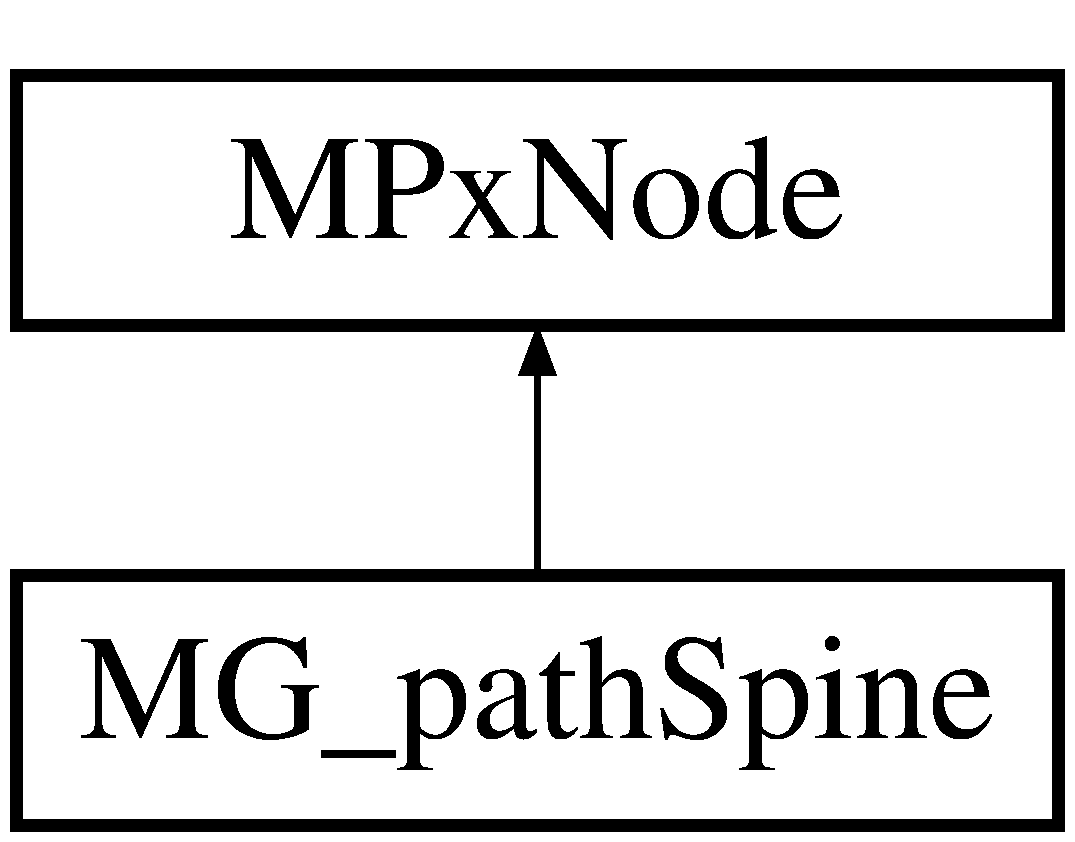
\includegraphics[height=2.000000cm]{class_m_g__path_spine}
\end{center}
\end{figure}
\subsection*{Public Member Functions}
\begin{DoxyCompactItemize}
\item 
\hypertarget{class_m_g__path_spine_a99684427fff3fbdb3137ca170d837006}{virtual M\-Status {\bfseries compute} (const M\-Plug \&plug, M\-Data\-Block \&data)}\label{class_m_g__path_spine_a99684427fff3fbdb3137ca170d837006}

\end{DoxyCompactItemize}
\subsection*{Static Public Member Functions}
\begin{DoxyCompactItemize}
\item 
\hypertarget{class_m_g__path_spine_ad76fe22353cfb17b5304fdb5983b11b3}{static void $\ast$ {\bfseries creator} ()}\label{class_m_g__path_spine_ad76fe22353cfb17b5304fdb5983b11b3}

\item 
\hypertarget{class_m_g__path_spine_a8df28dcaabc6098519fc0f7519425cc9}{static M\-Status {\bfseries initialize} ()}\label{class_m_g__path_spine_a8df28dcaabc6098519fc0f7519425cc9}

\end{DoxyCompactItemize}
\subsection*{Static Public Attributes}
\begin{DoxyCompactItemize}
\item 
static M\-Type\-Id \hyperlink{class_m_g__path_spine_a151a6bc4963051bb3ceb6cd45b5e51fc}{type\-Id}
\item 
static M\-Object \hyperlink{class_m_g__path_spine_ab44d5346a186856f9cee0e0b4b50b6b7}{input\-Curve}
\item 
static M\-Object \hyperlink{class_m_g__path_spine_afc674fb8cad25f40d47c292696b1737d}{first\-Up\-Vec}
\item 
static M\-Object \hyperlink{class_m_g__path_spine_aba3135fe0e05c181f1123510fec9118d}{first\-Up\-Vec\-X}
\item 
static M\-Object \hyperlink{class_m_g__path_spine_a681e0163d082d9e5b9ba0362b45ac58c}{first\-Up\-Vec\-Y}
\item 
static M\-Object \hyperlink{class_m_g__path_spine_aae8d7d46c33e1da9fae50fc557fa7b71}{first\-Up\-Vec\-Z}
\item 
static M\-Object \hyperlink{class_m_g__path_spine_a8b4339da0fdb021a6b91d1449c99732a}{output\-Translate\-X}
\item 
static M\-Object \hyperlink{class_m_g__path_spine_ab4aca6c192a9818ab64096edf8aaea0d}{output\-Translate\-Y}
\item 
static M\-Object \hyperlink{class_m_g__path_spine_ac19e9b5e38b171a158692ce31204dc1b}{output\-Translate\-Z}
\item 
static M\-Object \hyperlink{class_m_g__path_spine_a459813326a0970b67a4d94798a47aaba}{output\-Translate}
\item 
static M\-Object \hyperlink{class_m_g__path_spine_a5d73906fe1c6ec0b372c0ef3da2a0026}{output\-Rotate\-X}
\item 
static M\-Object \hyperlink{class_m_g__path_spine_a11b0bb32a6931055ec6d06b595f11b7e}{output\-Rotate\-Y}
\item 
static M\-Object \hyperlink{class_m_g__path_spine_a7449fba41f2530d7fa797d392beeb0e0}{output\-Rotate\-Z}
\item 
static M\-Object \hyperlink{class_m_g__path_spine_aa9044a045524a44c3d322c979cc9b8e8}{output\-Rotate}
\item 
static M\-Object \hyperlink{class_m_g__path_spine_a34a92ba0bc42a34ff70602b136272a01}{output\-Scale\-X}
\item 
static M\-Object \hyperlink{class_m_g__path_spine_a5cbcb31bcb281e841905b6ec643ce5bc}{output\-Scale\-Y}
\item 
static M\-Object \hyperlink{class_m_g__path_spine_a6708ed79d1460a01cffc3171889e1637}{output\-Scale\-Z}
\item 
static M\-Object \hyperlink{class_m_g__path_spine_a3c6c85e54a0a8f98f067df5884006717}{output\-Scale}
\item 
static M\-Object \hyperlink{class_m_g__path_spine_a1b03cd5d5735caea252ae5cc7f28a53c}{number\-Of\-Samples}
\item 
static M\-Object \hyperlink{class_m_g__path_spine_aed8434ed311d207b479f4418ca1bb432}{number\-Of\-Output}
\item 
static M\-Object \hyperlink{class_m_g__path_spine_a8eddab32708caeddc2c871d39e5d92fd}{parent\-Matrix}
\item 
static M\-Object \hyperlink{class_m_g__path_spine_a406a9df2d612bd346d3f7aac59646470}{start\-Length}
\item 
static M\-Object \hyperlink{class_m_g__path_spine_a56805052d8bd4e130c192b000b750efc}{stretch}
\item 
static M\-Object \hyperlink{class_m_g__path_spine_a3a8e37960ae8c40d2bf7cfe45ffcaaa6}{twist1}
\item 
static M\-Object \hyperlink{class_m_g__path_spine_a2558520e0fa84c73b1c52cfb9268ecab}{twist2}
\item 
static M\-Object \hyperlink{class_m_g__path_spine_a552a798b225b9aa4924e8d0d2c421843}{stretch\-Shape}
\item 
static M\-Object \hyperlink{class_m_g__path_spine_ab28430d046de80302091ba8be2c1ba8f}{squash\-Shape}
\item 
static M\-Object \hyperlink{class_m_g__path_spine_acfb6a9d96aadcc5630153819140993bb}{stretch\-Mult}
\item 
static M\-Object \hyperlink{class_m_g__path_spine_a9af9d259a81115c7fef275c67d54ccb1}{squash\-Mult}
\item 
static M\-Object \hyperlink{class_m_g__path_spine_a4c6cb4b1690e8704961a9e9a103c47a0}{keep\-Twist\-Volume}
\item 
static M\-Object \hyperlink{class_m_g__path_spine_adc3fed052e585c7b2f8345774c8e2d86}{keep\-Twist\-Volume\-Mult}
\item 
static M\-Object \hyperlink{class_m_g__path_spine_a89a8f6f283deb9da030ed711a78c1b3b}{twist\-Shape}
\item 
static M\-Object \hyperlink{class_m_g__path_spine_a61634d056e477a73db2a5c5bcfacec0a}{compute\-Twist}
\item 
static M\-Object \hyperlink{class_m_g__path_spine_ae23dd8337d46df00656630b0461c28df}{compute\-Volume\-Stretch}
\item 
static M\-Object \hyperlink{class_m_g__path_spine_a388952b4b3257d4ba2c7becb63a60061}{compute\-Volume\-Squash}
\item 
static M\-Object \hyperlink{class_m_g__path_spine_a2b442386812642012d95aecacc5939c1}{global\-Scale}
\end{DoxyCompactItemize}


\subsection{Detailed Description}
lets build a fast and flexible spine 

\begin{DoxyAuthor}{Author}
Marco Giordano 
\end{DoxyAuthor}
\begin{DoxyDate}{Date}
02/10/2013 
\end{DoxyDate}
\begin{DoxyVersion}{Version}
latest version \-: V1 

changeload versions \-: \par
 V1 \-: \par

\begin{DoxyItemize}
\item initial release \par

\end{DoxyItemize}
\end{DoxyVersion}
node name \-: \hyperlink{class_m_g__path_spine}{M\-G\-\_\-path\-Spine}.

details \-: This node lets build a fast and flexible spine with a lot of features like hardcore twisting , squash and stretch and more. N\-B \-: this nodes have as output severl arrays (translate ,rotate and scale), maya is really picky about arrays , if you try to acces an index that is not there well your going to crash. In order to avoid that be sure that the value of the attribute \char`\"{}number of outputs\char`\"{} is equal at the number of index in all output array , even if you dont conncet them create the index , otherwise the compute wont start. Example if you have number of outputs \-: 20 you will need to have as last index for example output\-Translate\mbox{[}19\mbox{]} , (array index count starts from 0 ). In order to create index if you dont have to connect them you can simply use a get\-Attr command on the indexes. Also be sure to set the start length value of the curve. I really hope someone from the community will provide scripts to hook up the node , I did it for myself but it s based on my pipeline I am currently developing so I can't share.

example create node \-: (M\-E\-L) create\-Node \hyperlink{class_m_g__path_spine}{M\-G\-\_\-path\-Spine}. 

\subsection{Member Data Documentation}
\hypertarget{class_m_g__path_spine_a61634d056e477a73db2a5c5bcfacec0a}{\index{M\-G\-\_\-path\-Spine@{M\-G\-\_\-path\-Spine}!compute\-Twist@{compute\-Twist}}
\index{compute\-Twist@{compute\-Twist}!MG_pathSpine@{M\-G\-\_\-path\-Spine}}
\subsubsection[{compute\-Twist}]{\setlength{\rightskip}{0pt plus 5cm}M\-Object M\-G\-\_\-path\-Spine\-::compute\-Twist\hspace{0.3cm}{\ttfamily [static]}}}\label{class_m_g__path_spine_a61634d056e477a73db2a5c5bcfacec0a}
This attribute turns on/off the computation of the twist \hypertarget{class_m_g__path_spine_a388952b4b3257d4ba2c7becb63a60061}{\index{M\-G\-\_\-path\-Spine@{M\-G\-\_\-path\-Spine}!compute\-Volume\-Squash@{compute\-Volume\-Squash}}
\index{compute\-Volume\-Squash@{compute\-Volume\-Squash}!MG_pathSpine@{M\-G\-\_\-path\-Spine}}
\subsubsection[{compute\-Volume\-Squash}]{\setlength{\rightskip}{0pt plus 5cm}M\-Object M\-G\-\_\-path\-Spine\-::compute\-Volume\-Squash\hspace{0.3cm}{\ttfamily [static]}}}\label{class_m_g__path_spine_a388952b4b3257d4ba2c7becb63a60061}
This attribute turns on/off the computation of the squash volume \hypertarget{class_m_g__path_spine_ae23dd8337d46df00656630b0461c28df}{\index{M\-G\-\_\-path\-Spine@{M\-G\-\_\-path\-Spine}!compute\-Volume\-Stretch@{compute\-Volume\-Stretch}}
\index{compute\-Volume\-Stretch@{compute\-Volume\-Stretch}!MG_pathSpine@{M\-G\-\_\-path\-Spine}}
\subsubsection[{compute\-Volume\-Stretch}]{\setlength{\rightskip}{0pt plus 5cm}M\-Object M\-G\-\_\-path\-Spine\-::compute\-Volume\-Stretch\hspace{0.3cm}{\ttfamily [static]}}}\label{class_m_g__path_spine_ae23dd8337d46df00656630b0461c28df}
This attribute turns on/off the computation of the stretch volume \hypertarget{class_m_g__path_spine_afc674fb8cad25f40d47c292696b1737d}{\index{M\-G\-\_\-path\-Spine@{M\-G\-\_\-path\-Spine}!first\-Up\-Vec@{first\-Up\-Vec}}
\index{first\-Up\-Vec@{first\-Up\-Vec}!MG_pathSpine@{M\-G\-\_\-path\-Spine}}
\subsubsection[{first\-Up\-Vec}]{\setlength{\rightskip}{0pt plus 5cm}M\-Object M\-G\-\_\-path\-Spine\-::first\-Up\-Vec\hspace{0.3cm}{\ttfamily [static]}}}\label{class_m_g__path_spine_afc674fb8cad25f40d47c292696b1737d}
This attribute holds the first up vector used to compute the normals on the curve \hypertarget{class_m_g__path_spine_aba3135fe0e05c181f1123510fec9118d}{\index{M\-G\-\_\-path\-Spine@{M\-G\-\_\-path\-Spine}!first\-Up\-Vec\-X@{first\-Up\-Vec\-X}}
\index{first\-Up\-Vec\-X@{first\-Up\-Vec\-X}!MG_pathSpine@{M\-G\-\_\-path\-Spine}}
\subsubsection[{first\-Up\-Vec\-X}]{\setlength{\rightskip}{0pt plus 5cm}M\-Object M\-G\-\_\-path\-Spine\-::first\-Up\-Vec\-X\hspace{0.3cm}{\ttfamily [static]}}}\label{class_m_g__path_spine_aba3135fe0e05c181f1123510fec9118d}
This attribute holds the X component of the first up vector used to compute the normals on the curve \hypertarget{class_m_g__path_spine_a681e0163d082d9e5b9ba0362b45ac58c}{\index{M\-G\-\_\-path\-Spine@{M\-G\-\_\-path\-Spine}!first\-Up\-Vec\-Y@{first\-Up\-Vec\-Y}}
\index{first\-Up\-Vec\-Y@{first\-Up\-Vec\-Y}!MG_pathSpine@{M\-G\-\_\-path\-Spine}}
\subsubsection[{first\-Up\-Vec\-Y}]{\setlength{\rightskip}{0pt plus 5cm}M\-Object M\-G\-\_\-path\-Spine\-::first\-Up\-Vec\-Y\hspace{0.3cm}{\ttfamily [static]}}}\label{class_m_g__path_spine_a681e0163d082d9e5b9ba0362b45ac58c}
This attribute holds the Y component of the first up vector used to compute the normals on the curve \hypertarget{class_m_g__path_spine_aae8d7d46c33e1da9fae50fc557fa7b71}{\index{M\-G\-\_\-path\-Spine@{M\-G\-\_\-path\-Spine}!first\-Up\-Vec\-Z@{first\-Up\-Vec\-Z}}
\index{first\-Up\-Vec\-Z@{first\-Up\-Vec\-Z}!MG_pathSpine@{M\-G\-\_\-path\-Spine}}
\subsubsection[{first\-Up\-Vec\-Z}]{\setlength{\rightskip}{0pt plus 5cm}M\-Object M\-G\-\_\-path\-Spine\-::first\-Up\-Vec\-Z\hspace{0.3cm}{\ttfamily [static]}}}\label{class_m_g__path_spine_aae8d7d46c33e1da9fae50fc557fa7b71}
This attribute holds the Z component of the first up vector used to compute the normals on the curve \hypertarget{class_m_g__path_spine_a2b442386812642012d95aecacc5939c1}{\index{M\-G\-\_\-path\-Spine@{M\-G\-\_\-path\-Spine}!global\-Scale@{global\-Scale}}
\index{global\-Scale@{global\-Scale}!MG_pathSpine@{M\-G\-\_\-path\-Spine}}
\subsubsection[{global\-Scale}]{\setlength{\rightskip}{0pt plus 5cm}M\-Object M\-G\-\_\-path\-Spine\-::global\-Scale\hspace{0.3cm}{\ttfamily [static]}}}\label{class_m_g__path_spine_a2b442386812642012d95aecacc5939c1}
T\-His attribute is used to fix global scale of the spine \hypertarget{class_m_g__path_spine_ab44d5346a186856f9cee0e0b4b50b6b7}{\index{M\-G\-\_\-path\-Spine@{M\-G\-\_\-path\-Spine}!input\-Curve@{input\-Curve}}
\index{input\-Curve@{input\-Curve}!MG_pathSpine@{M\-G\-\_\-path\-Spine}}
\subsubsection[{input\-Curve}]{\setlength{\rightskip}{0pt plus 5cm}M\-Object M\-G\-\_\-path\-Spine\-::input\-Curve\hspace{0.3cm}{\ttfamily [static]}}}\label{class_m_g__path_spine_ab44d5346a186856f9cee0e0b4b50b6b7}
This is the input curve value \hypertarget{class_m_g__path_spine_a4c6cb4b1690e8704961a9e9a103c47a0}{\index{M\-G\-\_\-path\-Spine@{M\-G\-\_\-path\-Spine}!keep\-Twist\-Volume@{keep\-Twist\-Volume}}
\index{keep\-Twist\-Volume@{keep\-Twist\-Volume}!MG_pathSpine@{M\-G\-\_\-path\-Spine}}
\subsubsection[{keep\-Twist\-Volume}]{\setlength{\rightskip}{0pt plus 5cm}M\-Object M\-G\-\_\-path\-Spine\-::keep\-Twist\-Volume\hspace{0.3cm}{\ttfamily [static]}}}\label{class_m_g__path_spine_a4c6cb4b1690e8704961a9e9a103c47a0}
This attribute define if to keep volume during twist or not \hypertarget{class_m_g__path_spine_adc3fed052e585c7b2f8345774c8e2d86}{\index{M\-G\-\_\-path\-Spine@{M\-G\-\_\-path\-Spine}!keep\-Twist\-Volume\-Mult@{keep\-Twist\-Volume\-Mult}}
\index{keep\-Twist\-Volume\-Mult@{keep\-Twist\-Volume\-Mult}!MG_pathSpine@{M\-G\-\_\-path\-Spine}}
\subsubsection[{keep\-Twist\-Volume\-Mult}]{\setlength{\rightskip}{0pt plus 5cm}M\-Object M\-G\-\_\-path\-Spine\-::keep\-Twist\-Volume\-Mult\hspace{0.3cm}{\ttfamily [static]}}}\label{class_m_g__path_spine_adc3fed052e585c7b2f8345774c8e2d86}
This attribute is used to multiply the keep\-Twist\-Volume amount \hypertarget{class_m_g__path_spine_aed8434ed311d207b479f4418ca1bb432}{\index{M\-G\-\_\-path\-Spine@{M\-G\-\_\-path\-Spine}!number\-Of\-Output@{number\-Of\-Output}}
\index{number\-Of\-Output@{number\-Of\-Output}!MG_pathSpine@{M\-G\-\_\-path\-Spine}}
\subsubsection[{number\-Of\-Output}]{\setlength{\rightskip}{0pt plus 5cm}M\-Object M\-G\-\_\-path\-Spine\-::number\-Of\-Output\hspace{0.3cm}{\ttfamily [static]}}}\label{class_m_g__path_spine_aed8434ed311d207b479f4418ca1bb432}
This attribute sets how many outputs will be computed \hypertarget{class_m_g__path_spine_a1b03cd5d5735caea252ae5cc7f28a53c}{\index{M\-G\-\_\-path\-Spine@{M\-G\-\_\-path\-Spine}!number\-Of\-Samples@{number\-Of\-Samples}}
\index{number\-Of\-Samples@{number\-Of\-Samples}!MG_pathSpine@{M\-G\-\_\-path\-Spine}}
\subsubsection[{number\-Of\-Samples}]{\setlength{\rightskip}{0pt plus 5cm}M\-Object M\-G\-\_\-path\-Spine\-::number\-Of\-Samples\hspace{0.3cm}{\ttfamily [static]}}}\label{class_m_g__path_spine_a1b03cd5d5735caea252ae5cc7f28a53c}
$\ast$\-This value sets how many samples are going to be done on the curve , the higher it is the more accurate $\ast$is the computation , of course with drops on performance , set a value that gives you the wanted result it has to be higher then then number of outputs , I usually keep it twice the number of outut \hypertarget{class_m_g__path_spine_aa9044a045524a44c3d322c979cc9b8e8}{\index{M\-G\-\_\-path\-Spine@{M\-G\-\_\-path\-Spine}!output\-Rotate@{output\-Rotate}}
\index{output\-Rotate@{output\-Rotate}!MG_pathSpine@{M\-G\-\_\-path\-Spine}}
\subsubsection[{output\-Rotate}]{\setlength{\rightskip}{0pt plus 5cm}M\-Object M\-G\-\_\-path\-Spine\-::output\-Rotate\hspace{0.3cm}{\ttfamily [static]}}}\label{class_m_g__path_spine_aa9044a045524a44c3d322c979cc9b8e8}
This is the output Rotate array \hypertarget{class_m_g__path_spine_a5d73906fe1c6ec0b372c0ef3da2a0026}{\index{M\-G\-\_\-path\-Spine@{M\-G\-\_\-path\-Spine}!output\-Rotate\-X@{output\-Rotate\-X}}
\index{output\-Rotate\-X@{output\-Rotate\-X}!MG_pathSpine@{M\-G\-\_\-path\-Spine}}
\subsubsection[{output\-Rotate\-X}]{\setlength{\rightskip}{0pt plus 5cm}M\-Object M\-G\-\_\-path\-Spine\-::output\-Rotate\-X\hspace{0.3cm}{\ttfamily [static]}}}\label{class_m_g__path_spine_a5d73906fe1c6ec0b372c0ef3da2a0026}
This is the X component of the output Rotate array \hypertarget{class_m_g__path_spine_a11b0bb32a6931055ec6d06b595f11b7e}{\index{M\-G\-\_\-path\-Spine@{M\-G\-\_\-path\-Spine}!output\-Rotate\-Y@{output\-Rotate\-Y}}
\index{output\-Rotate\-Y@{output\-Rotate\-Y}!MG_pathSpine@{M\-G\-\_\-path\-Spine}}
\subsubsection[{output\-Rotate\-Y}]{\setlength{\rightskip}{0pt plus 5cm}M\-Object M\-G\-\_\-path\-Spine\-::output\-Rotate\-Y\hspace{0.3cm}{\ttfamily [static]}}}\label{class_m_g__path_spine_a11b0bb32a6931055ec6d06b595f11b7e}
This is the Y component of the output Rotate array \hypertarget{class_m_g__path_spine_a7449fba41f2530d7fa797d392beeb0e0}{\index{M\-G\-\_\-path\-Spine@{M\-G\-\_\-path\-Spine}!output\-Rotate\-Z@{output\-Rotate\-Z}}
\index{output\-Rotate\-Z@{output\-Rotate\-Z}!MG_pathSpine@{M\-G\-\_\-path\-Spine}}
\subsubsection[{output\-Rotate\-Z}]{\setlength{\rightskip}{0pt plus 5cm}M\-Object M\-G\-\_\-path\-Spine\-::output\-Rotate\-Z\hspace{0.3cm}{\ttfamily [static]}}}\label{class_m_g__path_spine_a7449fba41f2530d7fa797d392beeb0e0}
This is the Z component of the output Rotate array \hypertarget{class_m_g__path_spine_a3c6c85e54a0a8f98f067df5884006717}{\index{M\-G\-\_\-path\-Spine@{M\-G\-\_\-path\-Spine}!output\-Scale@{output\-Scale}}
\index{output\-Scale@{output\-Scale}!MG_pathSpine@{M\-G\-\_\-path\-Spine}}
\subsubsection[{output\-Scale}]{\setlength{\rightskip}{0pt plus 5cm}M\-Object M\-G\-\_\-path\-Spine\-::output\-Scale\hspace{0.3cm}{\ttfamily [static]}}}\label{class_m_g__path_spine_a3c6c85e54a0a8f98f067df5884006717}
This is the output Scale array \hypertarget{class_m_g__path_spine_a34a92ba0bc42a34ff70602b136272a01}{\index{M\-G\-\_\-path\-Spine@{M\-G\-\_\-path\-Spine}!output\-Scale\-X@{output\-Scale\-X}}
\index{output\-Scale\-X@{output\-Scale\-X}!MG_pathSpine@{M\-G\-\_\-path\-Spine}}
\subsubsection[{output\-Scale\-X}]{\setlength{\rightskip}{0pt plus 5cm}M\-Object M\-G\-\_\-path\-Spine\-::output\-Scale\-X\hspace{0.3cm}{\ttfamily [static]}}}\label{class_m_g__path_spine_a34a92ba0bc42a34ff70602b136272a01}
This is the X component of the output Scale array \hypertarget{class_m_g__path_spine_a5cbcb31bcb281e841905b6ec643ce5bc}{\index{M\-G\-\_\-path\-Spine@{M\-G\-\_\-path\-Spine}!output\-Scale\-Y@{output\-Scale\-Y}}
\index{output\-Scale\-Y@{output\-Scale\-Y}!MG_pathSpine@{M\-G\-\_\-path\-Spine}}
\subsubsection[{output\-Scale\-Y}]{\setlength{\rightskip}{0pt plus 5cm}M\-Object M\-G\-\_\-path\-Spine\-::output\-Scale\-Y\hspace{0.3cm}{\ttfamily [static]}}}\label{class_m_g__path_spine_a5cbcb31bcb281e841905b6ec643ce5bc}
This is the Y component of the output Scale array \hypertarget{class_m_g__path_spine_a6708ed79d1460a01cffc3171889e1637}{\index{M\-G\-\_\-path\-Spine@{M\-G\-\_\-path\-Spine}!output\-Scale\-Z@{output\-Scale\-Z}}
\index{output\-Scale\-Z@{output\-Scale\-Z}!MG_pathSpine@{M\-G\-\_\-path\-Spine}}
\subsubsection[{output\-Scale\-Z}]{\setlength{\rightskip}{0pt plus 5cm}M\-Object M\-G\-\_\-path\-Spine\-::output\-Scale\-Z\hspace{0.3cm}{\ttfamily [static]}}}\label{class_m_g__path_spine_a6708ed79d1460a01cffc3171889e1637}
This is the Z component of the output Scale array \hypertarget{class_m_g__path_spine_a459813326a0970b67a4d94798a47aaba}{\index{M\-G\-\_\-path\-Spine@{M\-G\-\_\-path\-Spine}!output\-Translate@{output\-Translate}}
\index{output\-Translate@{output\-Translate}!MG_pathSpine@{M\-G\-\_\-path\-Spine}}
\subsubsection[{output\-Translate}]{\setlength{\rightskip}{0pt plus 5cm}M\-Object M\-G\-\_\-path\-Spine\-::output\-Translate\hspace{0.3cm}{\ttfamily [static]}}}\label{class_m_g__path_spine_a459813326a0970b67a4d94798a47aaba}
This is the output translate array \hypertarget{class_m_g__path_spine_a8b4339da0fdb021a6b91d1449c99732a}{\index{M\-G\-\_\-path\-Spine@{M\-G\-\_\-path\-Spine}!output\-Translate\-X@{output\-Translate\-X}}
\index{output\-Translate\-X@{output\-Translate\-X}!MG_pathSpine@{M\-G\-\_\-path\-Spine}}
\subsubsection[{output\-Translate\-X}]{\setlength{\rightskip}{0pt plus 5cm}M\-Object M\-G\-\_\-path\-Spine\-::output\-Translate\-X\hspace{0.3cm}{\ttfamily [static]}}}\label{class_m_g__path_spine_a8b4339da0fdb021a6b91d1449c99732a}
This is the X component of the output translate array \hypertarget{class_m_g__path_spine_ab4aca6c192a9818ab64096edf8aaea0d}{\index{M\-G\-\_\-path\-Spine@{M\-G\-\_\-path\-Spine}!output\-Translate\-Y@{output\-Translate\-Y}}
\index{output\-Translate\-Y@{output\-Translate\-Y}!MG_pathSpine@{M\-G\-\_\-path\-Spine}}
\subsubsection[{output\-Translate\-Y}]{\setlength{\rightskip}{0pt plus 5cm}M\-Object M\-G\-\_\-path\-Spine\-::output\-Translate\-Y\hspace{0.3cm}{\ttfamily [static]}}}\label{class_m_g__path_spine_ab4aca6c192a9818ab64096edf8aaea0d}
This is the Y component of the output translate array \hypertarget{class_m_g__path_spine_ac19e9b5e38b171a158692ce31204dc1b}{\index{M\-G\-\_\-path\-Spine@{M\-G\-\_\-path\-Spine}!output\-Translate\-Z@{output\-Translate\-Z}}
\index{output\-Translate\-Z@{output\-Translate\-Z}!MG_pathSpine@{M\-G\-\_\-path\-Spine}}
\subsubsection[{output\-Translate\-Z}]{\setlength{\rightskip}{0pt plus 5cm}M\-Object M\-G\-\_\-path\-Spine\-::output\-Translate\-Z\hspace{0.3cm}{\ttfamily [static]}}}\label{class_m_g__path_spine_ac19e9b5e38b171a158692ce31204dc1b}
This is the Z component of the output translate array \hypertarget{class_m_g__path_spine_a8eddab32708caeddc2c871d39e5d92fd}{\index{M\-G\-\_\-path\-Spine@{M\-G\-\_\-path\-Spine}!parent\-Matrix@{parent\-Matrix}}
\index{parent\-Matrix@{parent\-Matrix}!MG_pathSpine@{M\-G\-\_\-path\-Spine}}
\subsubsection[{parent\-Matrix}]{\setlength{\rightskip}{0pt plus 5cm}M\-Object M\-G\-\_\-path\-Spine\-::parent\-Matrix\hspace{0.3cm}{\ttfamily [static]}}}\label{class_m_g__path_spine_a8eddab32708caeddc2c871d39e5d92fd}
This attribute will hold the curve's transform world matrix \hypertarget{class_m_g__path_spine_a9af9d259a81115c7fef275c67d54ccb1}{\index{M\-G\-\_\-path\-Spine@{M\-G\-\_\-path\-Spine}!squash\-Mult@{squash\-Mult}}
\index{squash\-Mult@{squash\-Mult}!MG_pathSpine@{M\-G\-\_\-path\-Spine}}
\subsubsection[{squash\-Mult}]{\setlength{\rightskip}{0pt plus 5cm}M\-Object M\-G\-\_\-path\-Spine\-::squash\-Mult\hspace{0.3cm}{\ttfamily [static]}}}\label{class_m_g__path_spine_a9af9d259a81115c7fef275c67d54ccb1}
This attribute is used to multiply the value defined by the squash\-Shape \hypertarget{class_m_g__path_spine_ab28430d046de80302091ba8be2c1ba8f}{\index{M\-G\-\_\-path\-Spine@{M\-G\-\_\-path\-Spine}!squash\-Shape@{squash\-Shape}}
\index{squash\-Shape@{squash\-Shape}!MG_pathSpine@{M\-G\-\_\-path\-Spine}}
\subsubsection[{squash\-Shape}]{\setlength{\rightskip}{0pt plus 5cm}M\-Object M\-G\-\_\-path\-Spine\-::squash\-Shape\hspace{0.3cm}{\ttfamily [static]}}}\label{class_m_g__path_spine_ab28430d046de80302091ba8be2c1ba8f}
This attribute is used to define the shape of the squashed spine \hypertarget{class_m_g__path_spine_a406a9df2d612bd346d3f7aac59646470}{\index{M\-G\-\_\-path\-Spine@{M\-G\-\_\-path\-Spine}!start\-Length@{start\-Length}}
\index{start\-Length@{start\-Length}!MG_pathSpine@{M\-G\-\_\-path\-Spine}}
\subsubsection[{start\-Length}]{\setlength{\rightskip}{0pt plus 5cm}M\-Object M\-G\-\_\-path\-Spine\-::start\-Length\hspace{0.3cm}{\ttfamily [static]}}}\label{class_m_g__path_spine_a406a9df2d612bd346d3f7aac59646470}
This is the starth length of the curve and needs to be set manually \hypertarget{class_m_g__path_spine_a56805052d8bd4e130c192b000b750efc}{\index{M\-G\-\_\-path\-Spine@{M\-G\-\_\-path\-Spine}!stretch@{stretch}}
\index{stretch@{stretch}!MG_pathSpine@{M\-G\-\_\-path\-Spine}}
\subsubsection[{stretch}]{\setlength{\rightskip}{0pt plus 5cm}M\-Object M\-G\-\_\-path\-Spine\-::stretch\hspace{0.3cm}{\ttfamily [static]}}}\label{class_m_g__path_spine_a56805052d8bd4e130c192b000b750efc}
This attribute the amount of stretch along the curve \hypertarget{class_m_g__path_spine_acfb6a9d96aadcc5630153819140993bb}{\index{M\-G\-\_\-path\-Spine@{M\-G\-\_\-path\-Spine}!stretch\-Mult@{stretch\-Mult}}
\index{stretch\-Mult@{stretch\-Mult}!MG_pathSpine@{M\-G\-\_\-path\-Spine}}
\subsubsection[{stretch\-Mult}]{\setlength{\rightskip}{0pt plus 5cm}M\-Object M\-G\-\_\-path\-Spine\-::stretch\-Mult\hspace{0.3cm}{\ttfamily [static]}}}\label{class_m_g__path_spine_acfb6a9d96aadcc5630153819140993bb}
This attribute is used to multiply the value defined by the stretch\-Shape \hypertarget{class_m_g__path_spine_a552a798b225b9aa4924e8d0d2c421843}{\index{M\-G\-\_\-path\-Spine@{M\-G\-\_\-path\-Spine}!stretch\-Shape@{stretch\-Shape}}
\index{stretch\-Shape@{stretch\-Shape}!MG_pathSpine@{M\-G\-\_\-path\-Spine}}
\subsubsection[{stretch\-Shape}]{\setlength{\rightskip}{0pt plus 5cm}M\-Object M\-G\-\_\-path\-Spine\-::stretch\-Shape\hspace{0.3cm}{\ttfamily [static]}}}\label{class_m_g__path_spine_a552a798b225b9aa4924e8d0d2c421843}
This attribute is used to define the shape of the stretched spine \hypertarget{class_m_g__path_spine_a3a8e37960ae8c40d2bf7cfe45ffcaaa6}{\index{M\-G\-\_\-path\-Spine@{M\-G\-\_\-path\-Spine}!twist1@{twist1}}
\index{twist1@{twist1}!MG_pathSpine@{M\-G\-\_\-path\-Spine}}
\subsubsection[{twist1}]{\setlength{\rightskip}{0pt plus 5cm}M\-Object M\-G\-\_\-path\-Spine\-::twist1\hspace{0.3cm}{\ttfamily [static]}}}\label{class_m_g__path_spine_a3a8e37960ae8c40d2bf7cfe45ffcaaa6}
This is the input twist 1 \hypertarget{class_m_g__path_spine_a2558520e0fa84c73b1c52cfb9268ecab}{\index{M\-G\-\_\-path\-Spine@{M\-G\-\_\-path\-Spine}!twist2@{twist2}}
\index{twist2@{twist2}!MG_pathSpine@{M\-G\-\_\-path\-Spine}}
\subsubsection[{twist2}]{\setlength{\rightskip}{0pt plus 5cm}M\-Object M\-G\-\_\-path\-Spine\-::twist2\hspace{0.3cm}{\ttfamily [static]}}}\label{class_m_g__path_spine_a2558520e0fa84c73b1c52cfb9268ecab}
This is the input twist 2 \hypertarget{class_m_g__path_spine_a89a8f6f283deb9da030ed711a78c1b3b}{\index{M\-G\-\_\-path\-Spine@{M\-G\-\_\-path\-Spine}!twist\-Shape@{twist\-Shape}}
\index{twist\-Shape@{twist\-Shape}!MG_pathSpine@{M\-G\-\_\-path\-Spine}}
\subsubsection[{twist\-Shape}]{\setlength{\rightskip}{0pt plus 5cm}M\-Object M\-G\-\_\-path\-Spine\-::twist\-Shape\hspace{0.3cm}{\ttfamily [static]}}}\label{class_m_g__path_spine_a89a8f6f283deb9da030ed711a78c1b3b}
This attribute is used to define the shape of the twisted spine \hypertarget{class_m_g__path_spine_a151a6bc4963051bb3ceb6cd45b5e51fc}{\index{M\-G\-\_\-path\-Spine@{M\-G\-\_\-path\-Spine}!type\-Id@{type\-Id}}
\index{type\-Id@{type\-Id}!MG_pathSpine@{M\-G\-\_\-path\-Spine}}
\subsubsection[{type\-Id}]{\setlength{\rightskip}{0pt plus 5cm}M\-Type\-Id M\-G\-\_\-path\-Spine\-::type\-Id\hspace{0.3cm}{\ttfamily [static]}}}\label{class_m_g__path_spine_a151a6bc4963051bb3ceb6cd45b5e51fc}
The node id 

The documentation for this class was generated from the following file\-:\begin{DoxyCompactItemize}
\item 
C\-:/\-Users/giordi/\-Desktop/\-P\-R\-O\-G\-E\-T\-T\-I\-\_\-\-I\-N\-\_\-\-C\-O\-R\-S\-O/\-C/\-M\-G\-\_\-\-Tools/cpp/\-M\-G\-\_\-path\-Spine/src/M\-G\-\_\-path\-Spine.\-h\end{DoxyCompactItemize}

\hypertarget{class_m_g__poly_rivet}{\section{M\-G\-\_\-poly\-Rivet Class Reference}
\label{class_m_g__poly_rivet}\index{M\-G\-\_\-poly\-Rivet@{M\-G\-\_\-poly\-Rivet}}
}


lets you constraint an object on a poly mesh  




{\ttfamily \#include $<$M\-G\-\_\-poly\-Rivet.\-h$>$}

Inheritance diagram for M\-G\-\_\-poly\-Rivet\-:\begin{figure}[H]
\begin{center}
\leavevmode
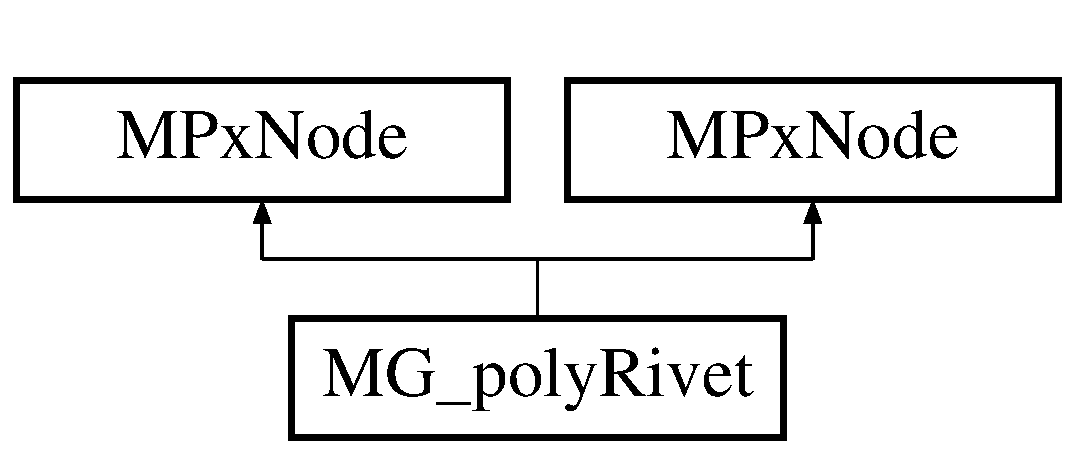
\includegraphics[height=2.000000cm]{class_m_g__poly_rivet}
\end{center}
\end{figure}
\subsection*{Public Member Functions}
\begin{DoxyCompactItemize}
\item 
\hypertarget{class_m_g__poly_rivet_a4dc8907a9f205585244e8e63c5264332}{virtual M\-Status {\bfseries compute} (const M\-Plug \&plug, M\-Data\-Block \&data\-Block)}\label{class_m_g__poly_rivet_a4dc8907a9f205585244e8e63c5264332}

\item 
\hypertarget{class_m_g__poly_rivet_a4dc8907a9f205585244e8e63c5264332}{virtual M\-Status {\bfseries compute} (const M\-Plug \&plug, M\-Data\-Block \&data\-Block)}\label{class_m_g__poly_rivet_a4dc8907a9f205585244e8e63c5264332}

\end{DoxyCompactItemize}
\subsection*{Static Public Member Functions}
\begin{DoxyCompactItemize}
\item 
\hypertarget{class_m_g__poly_rivet_acb96ab724745fe97361ba73416acc36f}{static void $\ast$ {\bfseries creator} ()}\label{class_m_g__poly_rivet_acb96ab724745fe97361ba73416acc36f}

\item 
\hypertarget{class_m_g__poly_rivet_af07102e7fa0ae367dc9469cfb04bbe3a}{static M\-Status {\bfseries initialize} ()}\label{class_m_g__poly_rivet_af07102e7fa0ae367dc9469cfb04bbe3a}

\item 
\hypertarget{class_m_g__poly_rivet_acb96ab724745fe97361ba73416acc36f}{static void $\ast$ {\bfseries creator} ()}\label{class_m_g__poly_rivet_acb96ab724745fe97361ba73416acc36f}

\item 
\hypertarget{class_m_g__poly_rivet_af07102e7fa0ae367dc9469cfb04bbe3a}{static M\-Status {\bfseries initialize} ()}\label{class_m_g__poly_rivet_af07102e7fa0ae367dc9469cfb04bbe3a}

\end{DoxyCompactItemize}
\subsection*{Static Public Attributes}
\begin{DoxyCompactItemize}
\item 
static M\-Object \hyperlink{class_m_g__poly_rivet_a7ab1746e551e796af0a8ded100097d23}{input\-Mesh}
\item 
static M\-Object \hyperlink{class_m_g__poly_rivet_af237dc390876f88e7577aa83457e7ce2}{input\-Point}
\item 
static M\-Object \hyperlink{class_m_g__poly_rivet_af74d6fe431dadcc1806a072cf97fba97}{recompute}
\item 
static M\-Object \hyperlink{class_m_g__poly_rivet_a3e4254e0cca1ba2be5fcbac82c9c5c12}{output}
\item 
static M\-Object \hyperlink{class_m_g__poly_rivet_a04be4b6c8cf58fe4b45bc20edbd52d38}{u\-Value}
\item 
static M\-Object \hyperlink{class_m_g__poly_rivet_aec3670f4f9a06480753efc8006076603}{v\-Value}
\item 
static M\-Object \hyperlink{class_m_g__poly_rivet_a258f5cda9a54d7c22b45c70c17852ffc}{output\-Rotate}
\item 
static M\-Object \hyperlink{class_m_g__poly_rivet_a66a9ea9bb7e75ba0c7bc1644dbbc481d}{output\-Matrix}
\item 
static M\-Object \hyperlink{class_m_g__poly_rivet_addab0e7cdd6ba7d9580198f19f66dbd0}{face\-Id}
\item 
static M\-Object \hyperlink{class_m_g__poly_rivet_a40686ba1ddd87b87272592bcbff78116}{offset\-Matrix}
\item 
static M\-Object \hyperlink{class_m_g__poly_rivet_a08e43c9e982462593cd8f161f7077f1c}{input\-Point\-X}
\item 
static M\-Object \hyperlink{class_m_g__poly_rivet_a2adde2d1b24113e0674eff68ac098cd5}{input\-Point\-Y}
\item 
static M\-Object \hyperlink{class_m_g__poly_rivet_ac16ba069fedb3f1e0b6991ab7f43891a}{input\-Point\-Z}
\item 
static M\-Object \hyperlink{class_m_g__poly_rivet_a71d0569c9b053861347de918d5c46b7b}{output\-X}
\item 
static M\-Object \hyperlink{class_m_g__poly_rivet_ab2fd560a86a5f12368660997fc166254}{output\-Y}
\item 
static M\-Object \hyperlink{class_m_g__poly_rivet_a7c80d2819ac2a76ca9feb872c4e3598d}{output\-Z}
\item 
static M\-Object \hyperlink{class_m_g__poly_rivet_a56e48fc9050adcabb9554e520335e6ab}{output\-Rotate\-X}
\item 
static M\-Object \hyperlink{class_m_g__poly_rivet_a2668b8ed6265a03068d1b9e52401330b}{output\-Rotate\-Y}
\item 
static M\-Object \hyperlink{class_m_g__poly_rivet_aae095981ed78cd7fddae65b96b2f54fa}{output\-Rotate\-Z}
\item 
static M\-Object \hyperlink{class_m_g__poly_rivet_a922ab768d29ec0c21e3fbdaad23e83ab}{mesh\-Parent\-Matrix}
\item 
static M\-Type\-Id \hyperlink{class_m_g__poly_rivet_ab40d934bc8164246ba36c1e2c96eaa7c}{type\-Id}
\end{DoxyCompactItemize}


\subsection{Detailed Description}
lets you constraint an object on a poly mesh 

\begin{DoxyAuthor}{Author}
Marco Giordano 
\end{DoxyAuthor}
\begin{DoxyDate}{Date}
10/26/2012 
\end{DoxyDate}
\begin{DoxyVersion}{Version}
latest version \-: V1 

changeload versions \-: \par
 V1 \-: \par

\begin{DoxyItemize}
\item initial release \par

\end{DoxyItemize}
\end{DoxyVersion}
node name \-: \hyperlink{class_m_g__poly_rivet}{M\-G\-\_\-poly\-Rivet}.

details \-: This node let you constraint an object on a poly mesh This node needs as input an input point, the input point is the point from where the closest point on the mesh will be calculated in order to place the rivet. An input mesh has to be provided , just connect the \char`\"{}world\-Mesh\char`\"{} attribute from the shape of the wanted mesh to input\-Surface attribute. If you want to keep an offset from the calculated rivet you can set the offset matrix in the node , this has to be calculate , I might provide a script for that in the feature. Also the world matrix from the mesh transform needs to be connected to mesh\-Parent\-Matrix attribute. Once your happy with the rivet position you can uncheck the recompute attribute , in this way the closest point on mesh wont be recomputed anymore , keep it on if you want to animate the i input point and slide the rivet on the mesh.

example create node \-: (M\-E\-L) create\-Node \hyperlink{class_m_g__poly_rivet}{M\-G\-\_\-poly\-Rivet}.

\begin{DoxyRefDesc}{Todo}
\item[\hyperlink{todo__todo000003}{Todo}]add baricentric coordinates computation mode\end{DoxyRefDesc}


\begin{DoxyAuthor}{Author}
Marco Giordano 
\end{DoxyAuthor}
\begin{DoxyDate}{Date}
10/26/2012 
\end{DoxyDate}
\begin{DoxyVersion}{Version}
latest version \-: V1 

changeload versions \-: \par
 V1 \-: \par

\begin{DoxyItemize}
\item initial release \par

\end{DoxyItemize}
\end{DoxyVersion}
node name \-: \hyperlink{class_m_g__poly_rivet}{M\-G\-\_\-poly\-Rivet}.

details \-: This node let you constraint an object on a poly mesh This node needs as input an input point, the input point is the point from where the closest point on the mesh will be calculated in order to place the rivet. An input mesh has to be provided , just connect the \char`\"{}world\-Mesh\char`\"{} attribute from the shape of the wanted mesh to input\-Surface attribute. If you want to keep an offset from the calculated rivet you can set the offset matrix in the node , this has to be calculate , I might provide a script for that in the feature. Also the world matrix from the mesh transform needs to be connected to mesh\-Parent\-Matrix attribute. Once your happy with the rivet position you can uncheck the recompute attribute , in this way the closest point on mesh wont be recomputed anymore , keep it on if you want to animate the i input point and slide the rivet on the mesh.

example create node \-: (M\-E\-L) create\-Node \hyperlink{class_m_g__poly_rivet}{M\-G\-\_\-poly\-Rivet}.

\begin{DoxyRefDesc}{Todo}
\item[\hyperlink{todo__todo000008}{Todo}]add baricentric coordinates computation mode\end{DoxyRefDesc}


\subsection{Member Data Documentation}
\hypertarget{class_m_g__poly_rivet_addab0e7cdd6ba7d9580198f19f66dbd0}{\index{M\-G\-\_\-poly\-Rivet@{M\-G\-\_\-poly\-Rivet}!face\-Id@{face\-Id}}
\index{face\-Id@{face\-Id}!MG_polyRivet@{M\-G\-\_\-poly\-Rivet}}
\subsubsection[{face\-Id}]{\setlength{\rightskip}{0pt plus 5cm}static M\-Object M\-G\-\_\-poly\-Rivet\-::face\-Id\hspace{0.3cm}{\ttfamily [static]}}}\label{class_m_g__poly_rivet_addab0e7cdd6ba7d9580198f19f66dbd0}
The face on which the rivet stays on \hypertarget{class_m_g__poly_rivet_a7ab1746e551e796af0a8ded100097d23}{\index{M\-G\-\_\-poly\-Rivet@{M\-G\-\_\-poly\-Rivet}!input\-Mesh@{input\-Mesh}}
\index{input\-Mesh@{input\-Mesh}!MG_polyRivet@{M\-G\-\_\-poly\-Rivet}}
\subsubsection[{input\-Mesh}]{\setlength{\rightskip}{0pt plus 5cm}static M\-Object M\-G\-\_\-poly\-Rivet\-::input\-Mesh\hspace{0.3cm}{\ttfamily [static]}}}\label{class_m_g__poly_rivet_a7ab1746e551e796af0a8ded100097d23}
Connect to this input the shape of the poly mesh on which the rivet will stay on \hypertarget{class_m_g__poly_rivet_af237dc390876f88e7577aa83457e7ce2}{\index{M\-G\-\_\-poly\-Rivet@{M\-G\-\_\-poly\-Rivet}!input\-Point@{input\-Point}}
\index{input\-Point@{input\-Point}!MG_polyRivet@{M\-G\-\_\-poly\-Rivet}}
\subsubsection[{input\-Point}]{\setlength{\rightskip}{0pt plus 5cm}static M\-Object M\-G\-\_\-poly\-Rivet\-::input\-Point\hspace{0.3cm}{\ttfamily [static]}}}\label{class_m_g__poly_rivet_af237dc390876f88e7577aa83457e7ce2}
This is the initial position for the target object \hypertarget{class_m_g__poly_rivet_a08e43c9e982462593cd8f161f7077f1c}{\index{M\-G\-\_\-poly\-Rivet@{M\-G\-\_\-poly\-Rivet}!input\-Point\-X@{input\-Point\-X}}
\index{input\-Point\-X@{input\-Point\-X}!MG_polyRivet@{M\-G\-\_\-poly\-Rivet}}
\subsubsection[{input\-Point\-X}]{\setlength{\rightskip}{0pt plus 5cm}static M\-Object M\-G\-\_\-poly\-Rivet\-::input\-Point\-X\hspace{0.3cm}{\ttfamily [static]}}}\label{class_m_g__poly_rivet_a08e43c9e982462593cd8f161f7077f1c}
The input X for the compound attribute input\-Point \hypertarget{class_m_g__poly_rivet_a2adde2d1b24113e0674eff68ac098cd5}{\index{M\-G\-\_\-poly\-Rivet@{M\-G\-\_\-poly\-Rivet}!input\-Point\-Y@{input\-Point\-Y}}
\index{input\-Point\-Y@{input\-Point\-Y}!MG_polyRivet@{M\-G\-\_\-poly\-Rivet}}
\subsubsection[{input\-Point\-Y}]{\setlength{\rightskip}{0pt plus 5cm}static M\-Object M\-G\-\_\-poly\-Rivet\-::input\-Point\-Y\hspace{0.3cm}{\ttfamily [static]}}}\label{class_m_g__poly_rivet_a2adde2d1b24113e0674eff68ac098cd5}
The input Y for the compound attribute input\-Point \hypertarget{class_m_g__poly_rivet_ac16ba069fedb3f1e0b6991ab7f43891a}{\index{M\-G\-\_\-poly\-Rivet@{M\-G\-\_\-poly\-Rivet}!input\-Point\-Z@{input\-Point\-Z}}
\index{input\-Point\-Z@{input\-Point\-Z}!MG_polyRivet@{M\-G\-\_\-poly\-Rivet}}
\subsubsection[{input\-Point\-Z}]{\setlength{\rightskip}{0pt plus 5cm}static M\-Object M\-G\-\_\-poly\-Rivet\-::input\-Point\-Z\hspace{0.3cm}{\ttfamily [static]}}}\label{class_m_g__poly_rivet_ac16ba069fedb3f1e0b6991ab7f43891a}
The input Z for the compound attribute input\-Point \hypertarget{class_m_g__poly_rivet_a922ab768d29ec0c21e3fbdaad23e83ab}{\index{M\-G\-\_\-poly\-Rivet@{M\-G\-\_\-poly\-Rivet}!mesh\-Parent\-Matrix@{mesh\-Parent\-Matrix}}
\index{mesh\-Parent\-Matrix@{mesh\-Parent\-Matrix}!MG_polyRivet@{M\-G\-\_\-poly\-Rivet}}
\subsubsection[{mesh\-Parent\-Matrix}]{\setlength{\rightskip}{0pt plus 5cm}static M\-Object M\-G\-\_\-poly\-Rivet\-::mesh\-Parent\-Matrix\hspace{0.3cm}{\ttfamily [static]}}}\label{class_m_g__poly_rivet_a922ab768d29ec0c21e3fbdaad23e83ab}
This attribute is the mesh transform world matrix used to multiply the $\ast$rivet matrix \hypertarget{class_m_g__poly_rivet_a40686ba1ddd87b87272592bcbff78116}{\index{M\-G\-\_\-poly\-Rivet@{M\-G\-\_\-poly\-Rivet}!offset\-Matrix@{offset\-Matrix}}
\index{offset\-Matrix@{offset\-Matrix}!MG_polyRivet@{M\-G\-\_\-poly\-Rivet}}
\subsubsection[{offset\-Matrix}]{\setlength{\rightskip}{0pt plus 5cm}static M\-Object M\-G\-\_\-poly\-Rivet\-::offset\-Matrix\hspace{0.3cm}{\ttfamily [static]}}}\label{class_m_g__poly_rivet_a40686ba1ddd87b87272592bcbff78116}
This attribute holds the offset matrix from the rivet to the target that is going to be driven by the rivet \hypertarget{class_m_g__poly_rivet_a3e4254e0cca1ba2be5fcbac82c9c5c12}{\index{M\-G\-\_\-poly\-Rivet@{M\-G\-\_\-poly\-Rivet}!output@{output}}
\index{output@{output}!MG_polyRivet@{M\-G\-\_\-poly\-Rivet}}
\subsubsection[{output}]{\setlength{\rightskip}{0pt plus 5cm}static M\-Object M\-G\-\_\-poly\-Rivet\-::output\hspace{0.3cm}{\ttfamily [static]}}}\label{class_m_g__poly_rivet_a3e4254e0cca1ba2be5fcbac82c9c5c12}
The output translate attribute \hypertarget{class_m_g__poly_rivet_a66a9ea9bb7e75ba0c7bc1644dbbc481d}{\index{M\-G\-\_\-poly\-Rivet@{M\-G\-\_\-poly\-Rivet}!output\-Matrix@{output\-Matrix}}
\index{output\-Matrix@{output\-Matrix}!MG_polyRivet@{M\-G\-\_\-poly\-Rivet}}
\subsubsection[{output\-Matrix}]{\setlength{\rightskip}{0pt plus 5cm}static M\-Object M\-G\-\_\-poly\-Rivet\-::output\-Matrix\hspace{0.3cm}{\ttfamily [static]}}}\label{class_m_g__poly_rivet_a66a9ea9bb7e75ba0c7bc1644dbbc481d}
The output matrix attribute \hypertarget{class_m_g__poly_rivet_a258f5cda9a54d7c22b45c70c17852ffc}{\index{M\-G\-\_\-poly\-Rivet@{M\-G\-\_\-poly\-Rivet}!output\-Rotate@{output\-Rotate}}
\index{output\-Rotate@{output\-Rotate}!MG_polyRivet@{M\-G\-\_\-poly\-Rivet}}
\subsubsection[{output\-Rotate}]{\setlength{\rightskip}{0pt plus 5cm}static M\-Object M\-G\-\_\-poly\-Rivet\-::output\-Rotate\hspace{0.3cm}{\ttfamily [static]}}}\label{class_m_g__poly_rivet_a258f5cda9a54d7c22b45c70c17852ffc}
The output rotate attribute \hypertarget{class_m_g__poly_rivet_a56e48fc9050adcabb9554e520335e6ab}{\index{M\-G\-\_\-poly\-Rivet@{M\-G\-\_\-poly\-Rivet}!output\-Rotate\-X@{output\-Rotate\-X}}
\index{output\-Rotate\-X@{output\-Rotate\-X}!MG_polyRivet@{M\-G\-\_\-poly\-Rivet}}
\subsubsection[{output\-Rotate\-X}]{\setlength{\rightskip}{0pt plus 5cm}static M\-Object M\-G\-\_\-poly\-Rivet\-::output\-Rotate\-X\hspace{0.3cm}{\ttfamily [static]}}}\label{class_m_g__poly_rivet_a56e48fc9050adcabb9554e520335e6ab}
The output X for the compound attribute output\-Rotate \hypertarget{class_m_g__poly_rivet_a2668b8ed6265a03068d1b9e52401330b}{\index{M\-G\-\_\-poly\-Rivet@{M\-G\-\_\-poly\-Rivet}!output\-Rotate\-Y@{output\-Rotate\-Y}}
\index{output\-Rotate\-Y@{output\-Rotate\-Y}!MG_polyRivet@{M\-G\-\_\-poly\-Rivet}}
\subsubsection[{output\-Rotate\-Y}]{\setlength{\rightskip}{0pt plus 5cm}static M\-Object M\-G\-\_\-poly\-Rivet\-::output\-Rotate\-Y\hspace{0.3cm}{\ttfamily [static]}}}\label{class_m_g__poly_rivet_a2668b8ed6265a03068d1b9e52401330b}
The output Y for the compound attribute output\-Rotate \hypertarget{class_m_g__poly_rivet_aae095981ed78cd7fddae65b96b2f54fa}{\index{M\-G\-\_\-poly\-Rivet@{M\-G\-\_\-poly\-Rivet}!output\-Rotate\-Z@{output\-Rotate\-Z}}
\index{output\-Rotate\-Z@{output\-Rotate\-Z}!MG_polyRivet@{M\-G\-\_\-poly\-Rivet}}
\subsubsection[{output\-Rotate\-Z}]{\setlength{\rightskip}{0pt plus 5cm}static M\-Object M\-G\-\_\-poly\-Rivet\-::output\-Rotate\-Z\hspace{0.3cm}{\ttfamily [static]}}}\label{class_m_g__poly_rivet_aae095981ed78cd7fddae65b96b2f54fa}
The output Z for the compound attribute output\-Rotate \hypertarget{class_m_g__poly_rivet_a71d0569c9b053861347de918d5c46b7b}{\index{M\-G\-\_\-poly\-Rivet@{M\-G\-\_\-poly\-Rivet}!output\-X@{output\-X}}
\index{output\-X@{output\-X}!MG_polyRivet@{M\-G\-\_\-poly\-Rivet}}
\subsubsection[{output\-X}]{\setlength{\rightskip}{0pt plus 5cm}static M\-Object M\-G\-\_\-poly\-Rivet\-::output\-X\hspace{0.3cm}{\ttfamily [static]}}}\label{class_m_g__poly_rivet_a71d0569c9b053861347de918d5c46b7b}
The output X for the compound attribute output \hypertarget{class_m_g__poly_rivet_ab2fd560a86a5f12368660997fc166254}{\index{M\-G\-\_\-poly\-Rivet@{M\-G\-\_\-poly\-Rivet}!output\-Y@{output\-Y}}
\index{output\-Y@{output\-Y}!MG_polyRivet@{M\-G\-\_\-poly\-Rivet}}
\subsubsection[{output\-Y}]{\setlength{\rightskip}{0pt plus 5cm}static M\-Object M\-G\-\_\-poly\-Rivet\-::output\-Y\hspace{0.3cm}{\ttfamily [static]}}}\label{class_m_g__poly_rivet_ab2fd560a86a5f12368660997fc166254}
The output Y for the compound attribute output \hypertarget{class_m_g__poly_rivet_a7c80d2819ac2a76ca9feb872c4e3598d}{\index{M\-G\-\_\-poly\-Rivet@{M\-G\-\_\-poly\-Rivet}!output\-Z@{output\-Z}}
\index{output\-Z@{output\-Z}!MG_polyRivet@{M\-G\-\_\-poly\-Rivet}}
\subsubsection[{output\-Z}]{\setlength{\rightskip}{0pt plus 5cm}static M\-Object M\-G\-\_\-poly\-Rivet\-::output\-Z\hspace{0.3cm}{\ttfamily [static]}}}\label{class_m_g__poly_rivet_a7c80d2819ac2a76ca9feb872c4e3598d}
The output Z for the compound attribute output \hypertarget{class_m_g__poly_rivet_af74d6fe431dadcc1806a072cf97fba97}{\index{M\-G\-\_\-poly\-Rivet@{M\-G\-\_\-poly\-Rivet}!recompute@{recompute}}
\index{recompute@{recompute}!MG_polyRivet@{M\-G\-\_\-poly\-Rivet}}
\subsubsection[{recompute}]{\setlength{\rightskip}{0pt plus 5cm}static M\-Object M\-G\-\_\-poly\-Rivet\-::recompute\hspace{0.3cm}{\ttfamily [static]}}}\label{class_m_g__poly_rivet_af74d6fe431dadcc1806a072cf97fba97}
This check box let you turn on of the recompute of the closest point on the poly\-Mesh \hypertarget{class_m_g__poly_rivet_ab40d934bc8164246ba36c1e2c96eaa7c}{\index{M\-G\-\_\-poly\-Rivet@{M\-G\-\_\-poly\-Rivet}!type\-Id@{type\-Id}}
\index{type\-Id@{type\-Id}!MG_polyRivet@{M\-G\-\_\-poly\-Rivet}}
\subsubsection[{type\-Id}]{\setlength{\rightskip}{0pt plus 5cm}static M\-Type\-Id M\-G\-\_\-poly\-Rivet\-::type\-Id\hspace{0.3cm}{\ttfamily [static]}}}\label{class_m_g__poly_rivet_ab40d934bc8164246ba36c1e2c96eaa7c}
The node id \hypertarget{class_m_g__poly_rivet_a04be4b6c8cf58fe4b45bc20edbd52d38}{\index{M\-G\-\_\-poly\-Rivet@{M\-G\-\_\-poly\-Rivet}!u\-Value@{u\-Value}}
\index{u\-Value@{u\-Value}!MG_polyRivet@{M\-G\-\_\-poly\-Rivet}}
\subsubsection[{u\-Value}]{\setlength{\rightskip}{0pt plus 5cm}static M\-Object M\-G\-\_\-poly\-Rivet\-::u\-Value\hspace{0.3cm}{\ttfamily [static]}}}\label{class_m_g__poly_rivet_a04be4b6c8cf58fe4b45bc20edbd52d38}
The u value for the rivet \hypertarget{class_m_g__poly_rivet_aec3670f4f9a06480753efc8006076603}{\index{M\-G\-\_\-poly\-Rivet@{M\-G\-\_\-poly\-Rivet}!v\-Value@{v\-Value}}
\index{v\-Value@{v\-Value}!MG_polyRivet@{M\-G\-\_\-poly\-Rivet}}
\subsubsection[{v\-Value}]{\setlength{\rightskip}{0pt plus 5cm}static M\-Object M\-G\-\_\-poly\-Rivet\-::v\-Value\hspace{0.3cm}{\ttfamily [static]}}}\label{class_m_g__poly_rivet_aec3670f4f9a06480753efc8006076603}
The v value for the rivet 

The documentation for this class was generated from the following files\-:\begin{DoxyCompactItemize}
\item 
C\-:/\-Users/giordi/\-Desktop/\-P\-R\-O\-G\-E\-T\-T\-I\-\_\-\-I\-N\-\_\-\-C\-O\-R\-S\-O/\-C/\-M\-G\-\_\-\-Tools/cpp/\-M\-G\-\_\-poly\-Rivet/src/M\-G\-\_\-poly\-Rivet.\-h\item 
C\-:/\-Users/giordi/\-Desktop/\-P\-R\-O\-G\-E\-T\-T\-I\-\_\-\-I\-N\-\_\-\-C\-O\-R\-S\-O/\-C/\-M\-G\-\_\-\-Tools/cpp/\-M\-G\-\_\-tools\-Lite/src/M\-G\-\_\-poly\-Rivet.\-h\end{DoxyCompactItemize}

\hypertarget{class_m_g__pose_reader}{\section{M\-G\-\_\-pose\-Reader Class Reference}
\label{class_m_g__pose_reader}\index{M\-G\-\_\-pose\-Reader@{M\-G\-\_\-pose\-Reader}}
}


This node let s you read a position based on a sperichal area.  




{\ttfamily \#include $<$M\-G\-\_\-pose\-Reader.\-h$>$}

Inheritance diagram for M\-G\-\_\-pose\-Reader\-:\begin{figure}[H]
\begin{center}
\leavevmode
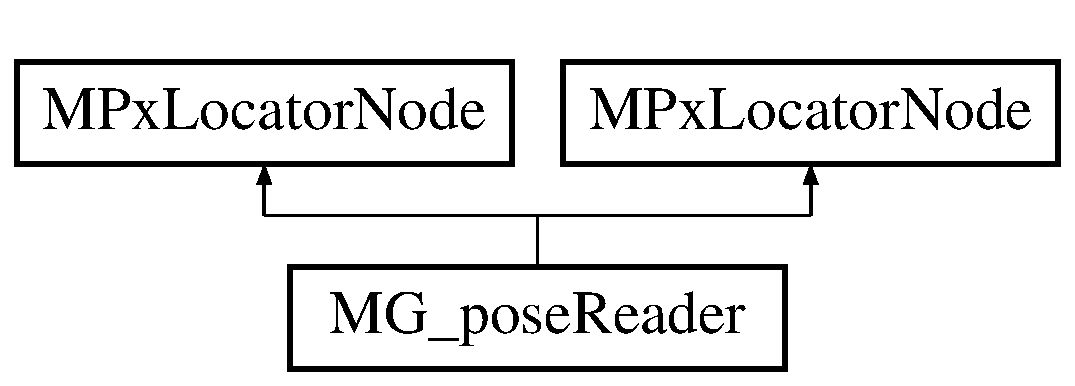
\includegraphics[height=2.000000cm]{class_m_g__pose_reader}
\end{center}
\end{figure}
\subsection*{Public Member Functions}
\begin{DoxyCompactItemize}
\item 
\hypertarget{class_m_g__pose_reader_ac5c3548456e3e65824f4fd817d7d03d6}{virtual M\-Status {\bfseries compute} (const M\-Plug \&plug, M\-Data\-Block \&data)}\label{class_m_g__pose_reader_ac5c3548456e3e65824f4fd817d7d03d6}

\item 
\hypertarget{class_m_g__pose_reader_a9e6b38a92e8fc372db1667930ca8d9ac}{virtual void {\bfseries draw} (M3d\-View \&, const M\-Dag\-Path \&, M3d\-View\-::\-Display\-Style, M3d\-View\-::\-Display\-Status)}\label{class_m_g__pose_reader_a9e6b38a92e8fc372db1667930ca8d9ac}

\item 
\hypertarget{class_m_g__pose_reader_a034a144161630705a28dfe12ddf3a54b}{virtual bool {\bfseries is\-Bounded} () const }\label{class_m_g__pose_reader_a034a144161630705a28dfe12ddf3a54b}

\item 
\hypertarget{class_m_g__pose_reader_ac5c3548456e3e65824f4fd817d7d03d6}{virtual M\-Status {\bfseries compute} (const M\-Plug \&plug, M\-Data\-Block \&data)}\label{class_m_g__pose_reader_ac5c3548456e3e65824f4fd817d7d03d6}

\item 
\hypertarget{class_m_g__pose_reader_a9e6b38a92e8fc372db1667930ca8d9ac}{virtual void {\bfseries draw} (M3d\-View \&, const M\-Dag\-Path \&, M3d\-View\-::\-Display\-Style, M3d\-View\-::\-Display\-Status)}\label{class_m_g__pose_reader_a9e6b38a92e8fc372db1667930ca8d9ac}

\item 
\hypertarget{class_m_g__pose_reader_a034a144161630705a28dfe12ddf3a54b}{virtual bool {\bfseries is\-Bounded} () const }\label{class_m_g__pose_reader_a034a144161630705a28dfe12ddf3a54b}

\end{DoxyCompactItemize}
\subsection*{Static Public Member Functions}
\begin{DoxyCompactItemize}
\item 
\hypertarget{class_m_g__pose_reader_a259ed1e21e2c0b5a5dc946968508bc21}{static void $\ast$ {\bfseries creator} ()}\label{class_m_g__pose_reader_a259ed1e21e2c0b5a5dc946968508bc21}

\item 
\hypertarget{class_m_g__pose_reader_acdc38f49889fe75116839e3c718857b5}{static M\-Status {\bfseries initialize} ()}\label{class_m_g__pose_reader_acdc38f49889fe75116839e3c718857b5}

\item 
\hypertarget{class_m_g__pose_reader_a259ed1e21e2c0b5a5dc946968508bc21}{static void $\ast$ {\bfseries creator} ()}\label{class_m_g__pose_reader_a259ed1e21e2c0b5a5dc946968508bc21}

\item 
\hypertarget{class_m_g__pose_reader_acdc38f49889fe75116839e3c718857b5}{static M\-Status {\bfseries initialize} ()}\label{class_m_g__pose_reader_acdc38f49889fe75116839e3c718857b5}

\end{DoxyCompactItemize}
\subsection*{Static Public Attributes}
\begin{DoxyCompactItemize}
\item 
static M\-Type\-Id \hyperlink{class_m_g__pose_reader_a0377069c7c81064a0102b87b43f17de7}{type\-Id}
\item 
static M\-Object \hyperlink{class_m_g__pose_reader_a8d13cb5a9150c21108b530211b1a5693}{reader\-Matrix}
\item 
static M\-Object \hyperlink{class_m_g__pose_reader_a37357d03b4a67aecbe5b3a7e3779cac7}{pose\-Matrix}
\item 
static M\-Object \hyperlink{class_m_g__pose_reader_a452750f9ea6f7d58cdd582666caf93aa}{size}
\item 
static M\-Object \hyperlink{class_m_g__pose_reader_ac0827c80b838e3536fea477045a4903d}{aim\-Axis}
\item 
static M\-Object \hyperlink{class_m_g__pose_reader_a431fdcb6a8e76c2963660dc58b7832c0}{reader\-On\-Off}
\item 
static M\-Object \hyperlink{class_m_g__pose_reader_a87e5e32106ddc45fbd15390698f1cbef}{axis\-On\-Off}
\item 
static M\-Object \hyperlink{class_m_g__pose_reader_a94faeca46f1634cb4634df288acad4f2}{pose\-On\-Off}
\item 
static M\-Object \hyperlink{class_m_g__pose_reader_a575eb3243593993d47794ede7e56a19a}{x\-Positive}
\item 
static M\-Object \hyperlink{class_m_g__pose_reader_a70a536b55c374d6fa3ee29da2d07e416}{x\-Negative}
\item 
static M\-Object \hyperlink{class_m_g__pose_reader_ad9eddeafae27cd633b869c5fc9dc4513}{y\-Positive}
\item 
static M\-Object \hyperlink{class_m_g__pose_reader_af45e2be7873bbfd49425fb622beae3d3}{y\-Negative}
\item 
static M\-Object \hyperlink{class_m_g__pose_reader_aef81fc58368214f0e34421990e6b53f8}{z\-Positive}
\item 
static M\-Object \hyperlink{class_m_g__pose_reader_aff4a284d37e399e1b3a8d1dbea31c3bc}{z\-Negative}
\end{DoxyCompactItemize}


\subsection{Detailed Description}
This node let s you read a position based on a sperichal area. 

\begin{DoxyAuthor}{Author}
Marco Giordano 
\end{DoxyAuthor}
\begin{DoxyDate}{Date}
10/26/2012 
\end{DoxyDate}
\begin{DoxyVersion}{Version}
latest version \-: V1 

changeload versions \-: \par
 V1 \-: \par

\begin{DoxyItemize}
\item initial release \par

\end{DoxyItemize}
\end{DoxyVersion}
node name \-: \hyperlink{class_m_g__pose_reader}{M\-G\-\_\-pose\-Reader}.

details \-: This node let s you read a position based on a sperichal area , perfect to trigger blendshapes or rig an autovlavicle and so on. Actually the autoclavicle rig was the reason why I wanted to create this plugin. This node needs the world space matrix of the pose\-Reader itself to be connected to the reader\-Matrix attribute. Beware that the pose\-Reader itself is a shape so you need to plug the relative transform world matrix. Then you have to connect the world matrix of the object you want to read the pose and also set what axis you want to take in consideration of this object. In the end you have just to plug the data you want to read , possible targets are
\begin{DoxyItemize}
\item +x
\item -\/x
\item +y
\item -\/y
\item +z
\item -\/z
\end{DoxyItemize}

example create node \-: (M\-E\-L) create\-Node \hyperlink{class_m_g__pose_reader}{M\-G\-\_\-pose\-Reader}.

\begin{DoxyRefDesc}{Todo}
\item[\hyperlink{todo__todo000004}{Todo}]implement torque reading\end{DoxyRefDesc}


\begin{DoxyAuthor}{Author}
Marco Giordano 
\end{DoxyAuthor}
\begin{DoxyDate}{Date}
10/26/2012 
\end{DoxyDate}
\begin{DoxyVersion}{Version}
latest version \-: V1 

changeload versions \-: \par
 V1 \-: \par

\begin{DoxyItemize}
\item initial release \par

\end{DoxyItemize}
\end{DoxyVersion}
node name \-: \hyperlink{class_m_g__pose_reader}{M\-G\-\_\-pose\-Reader}.

details \-: This node let s you read a position based on a sperichal area , perfect to trigger blendshapes or rig an autovlavicle and so on. Actually the autoclavicle rig was the reason why I wanted to create this plugin. This node needs the world space matrix of the pose\-Reader itself to be connected to the reader\-Matrix attribute. Beware that the pose\-Reader itself is a shape so you need to plug the relative transform world matrix. Then you have to connect the world matrix of the object you want to read the pose and also set what axis you want to take in consideration of this object. In the end you have just to plug the data you want to read , possible targets are
\begin{DoxyItemize}
\item +x
\item -\/x
\item +y
\item -\/y
\item +z
\item -\/z
\end{DoxyItemize}

example create node \-: (M\-E\-L) create\-Node \hyperlink{class_m_g__pose_reader}{M\-G\-\_\-pose\-Reader}.

\begin{DoxyRefDesc}{Todo}
\item[\hyperlink{todo__todo000009}{Todo}]implement torque reading\end{DoxyRefDesc}


\subsection{Member Data Documentation}
\hypertarget{class_m_g__pose_reader_ac0827c80b838e3536fea477045a4903d}{\index{M\-G\-\_\-pose\-Reader@{M\-G\-\_\-pose\-Reader}!aim\-Axis@{aim\-Axis}}
\index{aim\-Axis@{aim\-Axis}!MG_poseReader@{M\-G\-\_\-pose\-Reader}}
\subsubsection[{aim\-Axis}]{\setlength{\rightskip}{0pt plus 5cm}static M\-Object M\-G\-\_\-pose\-Reader\-::aim\-Axis\hspace{0.3cm}{\ttfamily [static]}}}\label{class_m_g__pose_reader_ac0827c80b838e3536fea477045a4903d}
Which axis to read of the object \hypertarget{class_m_g__pose_reader_a87e5e32106ddc45fbd15390698f1cbef}{\index{M\-G\-\_\-pose\-Reader@{M\-G\-\_\-pose\-Reader}!axis\-On\-Off@{axis\-On\-Off}}
\index{axis\-On\-Off@{axis\-On\-Off}!MG_poseReader@{M\-G\-\_\-pose\-Reader}}
\subsubsection[{axis\-On\-Off}]{\setlength{\rightskip}{0pt plus 5cm}static M\-Object M\-G\-\_\-pose\-Reader\-::axis\-On\-Off\hspace{0.3cm}{\ttfamily [static]}}}\label{class_m_g__pose_reader_a87e5e32106ddc45fbd15390698f1cbef}
This attribute sets if the axis targets are visible in viewport or not \hypertarget{class_m_g__pose_reader_a37357d03b4a67aecbe5b3a7e3779cac7}{\index{M\-G\-\_\-pose\-Reader@{M\-G\-\_\-pose\-Reader}!pose\-Matrix@{pose\-Matrix}}
\index{pose\-Matrix@{pose\-Matrix}!MG_poseReader@{M\-G\-\_\-pose\-Reader}}
\subsubsection[{pose\-Matrix}]{\setlength{\rightskip}{0pt plus 5cm}static M\-Object M\-G\-\_\-pose\-Reader\-::pose\-Matrix\hspace{0.3cm}{\ttfamily [static]}}}\label{class_m_g__pose_reader_a37357d03b4a67aecbe5b3a7e3779cac7}
The matrix of the object we want to read the pose \hypertarget{class_m_g__pose_reader_a94faeca46f1634cb4634df288acad4f2}{\index{M\-G\-\_\-pose\-Reader@{M\-G\-\_\-pose\-Reader}!pose\-On\-Off@{pose\-On\-Off}}
\index{pose\-On\-Off@{pose\-On\-Off}!MG_poseReader@{M\-G\-\_\-pose\-Reader}}
\subsubsection[{pose\-On\-Off}]{\setlength{\rightskip}{0pt plus 5cm}static M\-Object M\-G\-\_\-pose\-Reader\-::pose\-On\-Off\hspace{0.3cm}{\ttfamily [static]}}}\label{class_m_g__pose_reader_a94faeca46f1634cb4634df288acad4f2}
This attribute sets if the pose target is visible in viewport or not \hypertarget{class_m_g__pose_reader_a8d13cb5a9150c21108b530211b1a5693}{\index{M\-G\-\_\-pose\-Reader@{M\-G\-\_\-pose\-Reader}!reader\-Matrix@{reader\-Matrix}}
\index{reader\-Matrix@{reader\-Matrix}!MG_poseReader@{M\-G\-\_\-pose\-Reader}}
\subsubsection[{reader\-Matrix}]{\setlength{\rightskip}{0pt plus 5cm}static M\-Object M\-G\-\_\-pose\-Reader\-::reader\-Matrix\hspace{0.3cm}{\ttfamily [static]}}}\label{class_m_g__pose_reader_a8d13cb5a9150c21108b530211b1a5693}
$\ast$\-The world matrix of the pose\-Reader \hypertarget{class_m_g__pose_reader_a431fdcb6a8e76c2963660dc58b7832c0}{\index{M\-G\-\_\-pose\-Reader@{M\-G\-\_\-pose\-Reader}!reader\-On\-Off@{reader\-On\-Off}}
\index{reader\-On\-Off@{reader\-On\-Off}!MG_poseReader@{M\-G\-\_\-pose\-Reader}}
\subsubsection[{reader\-On\-Off}]{\setlength{\rightskip}{0pt plus 5cm}static M\-Object M\-G\-\_\-pose\-Reader\-::reader\-On\-Off\hspace{0.3cm}{\ttfamily [static]}}}\label{class_m_g__pose_reader_a431fdcb6a8e76c2963660dc58b7832c0}
This attribute sets if the reader is visible in viewport or not \hypertarget{class_m_g__pose_reader_a452750f9ea6f7d58cdd582666caf93aa}{\index{M\-G\-\_\-pose\-Reader@{M\-G\-\_\-pose\-Reader}!size@{size}}
\index{size@{size}!MG_poseReader@{M\-G\-\_\-pose\-Reader}}
\subsubsection[{size}]{\setlength{\rightskip}{0pt plus 5cm}static M\-Object M\-G\-\_\-pose\-Reader\-::size\hspace{0.3cm}{\ttfamily [static]}}}\label{class_m_g__pose_reader_a452750f9ea6f7d58cdd582666caf93aa}
The size of the pose\-Reader \hypertarget{class_m_g__pose_reader_a0377069c7c81064a0102b87b43f17de7}{\index{M\-G\-\_\-pose\-Reader@{M\-G\-\_\-pose\-Reader}!type\-Id@{type\-Id}}
\index{type\-Id@{type\-Id}!MG_poseReader@{M\-G\-\_\-pose\-Reader}}
\subsubsection[{type\-Id}]{\setlength{\rightskip}{0pt plus 5cm}static M\-Type\-Id M\-G\-\_\-pose\-Reader\-::type\-Id\hspace{0.3cm}{\ttfamily [static]}}}\label{class_m_g__pose_reader_a0377069c7c81064a0102b87b43f17de7}
The node id \hypertarget{class_m_g__pose_reader_a70a536b55c374d6fa3ee29da2d07e416}{\index{M\-G\-\_\-pose\-Reader@{M\-G\-\_\-pose\-Reader}!x\-Negative@{x\-Negative}}
\index{x\-Negative@{x\-Negative}!MG_poseReader@{M\-G\-\_\-pose\-Reader}}
\subsubsection[{x\-Negative}]{\setlength{\rightskip}{0pt plus 5cm}static M\-Object M\-G\-\_\-pose\-Reader\-::x\-Negative\hspace{0.3cm}{\ttfamily [static]}}}\label{class_m_g__pose_reader_a70a536b55c374d6fa3ee29da2d07e416}
the negative x value of the pose \hypertarget{class_m_g__pose_reader_a575eb3243593993d47794ede7e56a19a}{\index{M\-G\-\_\-pose\-Reader@{M\-G\-\_\-pose\-Reader}!x\-Positive@{x\-Positive}}
\index{x\-Positive@{x\-Positive}!MG_poseReader@{M\-G\-\_\-pose\-Reader}}
\subsubsection[{x\-Positive}]{\setlength{\rightskip}{0pt plus 5cm}static M\-Object M\-G\-\_\-pose\-Reader\-::x\-Positive\hspace{0.3cm}{\ttfamily [static]}}}\label{class_m_g__pose_reader_a575eb3243593993d47794ede7e56a19a}
the positive x value of the pose \hypertarget{class_m_g__pose_reader_af45e2be7873bbfd49425fb622beae3d3}{\index{M\-G\-\_\-pose\-Reader@{M\-G\-\_\-pose\-Reader}!y\-Negative@{y\-Negative}}
\index{y\-Negative@{y\-Negative}!MG_poseReader@{M\-G\-\_\-pose\-Reader}}
\subsubsection[{y\-Negative}]{\setlength{\rightskip}{0pt plus 5cm}static M\-Object M\-G\-\_\-pose\-Reader\-::y\-Negative\hspace{0.3cm}{\ttfamily [static]}}}\label{class_m_g__pose_reader_af45e2be7873bbfd49425fb622beae3d3}
the negative y value of the pose \hypertarget{class_m_g__pose_reader_ad9eddeafae27cd633b869c5fc9dc4513}{\index{M\-G\-\_\-pose\-Reader@{M\-G\-\_\-pose\-Reader}!y\-Positive@{y\-Positive}}
\index{y\-Positive@{y\-Positive}!MG_poseReader@{M\-G\-\_\-pose\-Reader}}
\subsubsection[{y\-Positive}]{\setlength{\rightskip}{0pt plus 5cm}static M\-Object M\-G\-\_\-pose\-Reader\-::y\-Positive\hspace{0.3cm}{\ttfamily [static]}}}\label{class_m_g__pose_reader_ad9eddeafae27cd633b869c5fc9dc4513}
the positive y value of the pose \hypertarget{class_m_g__pose_reader_aff4a284d37e399e1b3a8d1dbea31c3bc}{\index{M\-G\-\_\-pose\-Reader@{M\-G\-\_\-pose\-Reader}!z\-Negative@{z\-Negative}}
\index{z\-Negative@{z\-Negative}!MG_poseReader@{M\-G\-\_\-pose\-Reader}}
\subsubsection[{z\-Negative}]{\setlength{\rightskip}{0pt plus 5cm}static M\-Object M\-G\-\_\-pose\-Reader\-::z\-Negative\hspace{0.3cm}{\ttfamily [static]}}}\label{class_m_g__pose_reader_aff4a284d37e399e1b3a8d1dbea31c3bc}
the negative z value of the pose \hypertarget{class_m_g__pose_reader_aef81fc58368214f0e34421990e6b53f8}{\index{M\-G\-\_\-pose\-Reader@{M\-G\-\_\-pose\-Reader}!z\-Positive@{z\-Positive}}
\index{z\-Positive@{z\-Positive}!MG_poseReader@{M\-G\-\_\-pose\-Reader}}
\subsubsection[{z\-Positive}]{\setlength{\rightskip}{0pt plus 5cm}static M\-Object M\-G\-\_\-pose\-Reader\-::z\-Positive\hspace{0.3cm}{\ttfamily [static]}}}\label{class_m_g__pose_reader_aef81fc58368214f0e34421990e6b53f8}
the positive y value of the pose 

The documentation for this class was generated from the following files\-:\begin{DoxyCompactItemize}
\item 
C\-:/\-Users/giordi/\-Desktop/\-P\-R\-O\-G\-E\-T\-T\-I\-\_\-\-I\-N\-\_\-\-C\-O\-R\-S\-O/\-C/\-M\-G\-\_\-\-Tools/cpp/\-M\-G\-\_\-pose\-Reader/src/M\-G\-\_\-pose\-Reader.\-h\item 
C\-:/\-Users/giordi/\-Desktop/\-P\-R\-O\-G\-E\-T\-T\-I\-\_\-\-I\-N\-\_\-\-C\-O\-R\-S\-O/\-C/\-M\-G\-\_\-\-Tools/cpp/\-M\-G\-\_\-tools\-Lite/src/M\-G\-\_\-pose\-Reader.\-h\end{DoxyCompactItemize}

\hypertarget{class_m_g__spline_path}{\section{M\-G\-\_\-spline\-Path Class Reference}
\label{class_m_g__spline_path}\index{M\-G\-\_\-spline\-Path@{M\-G\-\_\-spline\-Path}}
}


lets you attach object on a curve and slide them  




{\ttfamily \#include $<$M\-G\-\_\-spline\-Path.\-h$>$}

Inheritance diagram for M\-G\-\_\-spline\-Path\-:\begin{figure}[H]
\begin{center}
\leavevmode
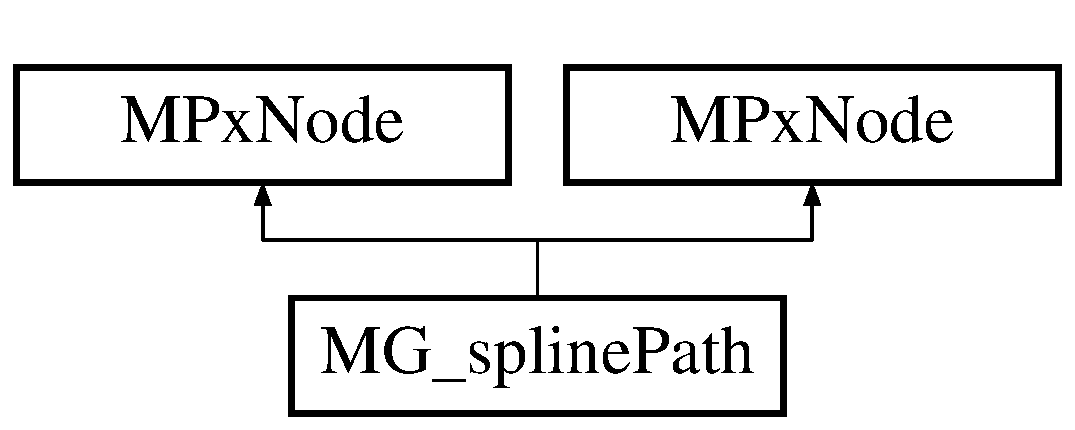
\includegraphics[height=2.000000cm]{class_m_g__spline_path}
\end{center}
\end{figure}
\subsection*{Public Member Functions}
\begin{DoxyCompactItemize}
\item 
\hypertarget{class_m_g__spline_path_a464608bab05012cf1ec3d4c1d30c12e3}{virtual M\-Status {\bfseries compute} (const M\-Plug \&plug, M\-Data\-Block \&data)}\label{class_m_g__spline_path_a464608bab05012cf1ec3d4c1d30c12e3}

\item 
\hypertarget{class_m_g__spline_path_a464608bab05012cf1ec3d4c1d30c12e3}{virtual M\-Status {\bfseries compute} (const M\-Plug \&plug, M\-Data\-Block \&data)}\label{class_m_g__spline_path_a464608bab05012cf1ec3d4c1d30c12e3}

\end{DoxyCompactItemize}
\subsection*{Static Public Member Functions}
\begin{DoxyCompactItemize}
\item 
\hypertarget{class_m_g__spline_path_ab3ed6a2caeb81d72c17b0dee7d70e628}{static void $\ast$ {\bfseries creator} ()}\label{class_m_g__spline_path_ab3ed6a2caeb81d72c17b0dee7d70e628}

\item 
\hypertarget{class_m_g__spline_path_a50a117d16a57029b4377836b6e843556}{static M\-Status {\bfseries initialize} ()}\label{class_m_g__spline_path_a50a117d16a57029b4377836b6e843556}

\item 
\hypertarget{class_m_g__spline_path_ab3ed6a2caeb81d72c17b0dee7d70e628}{static void $\ast$ {\bfseries creator} ()}\label{class_m_g__spline_path_ab3ed6a2caeb81d72c17b0dee7d70e628}

\item 
\hypertarget{class_m_g__spline_path_a50a117d16a57029b4377836b6e843556}{static M\-Status {\bfseries initialize} ()}\label{class_m_g__spline_path_a50a117d16a57029b4377836b6e843556}

\end{DoxyCompactItemize}
\subsection*{Static Public Attributes}
\begin{DoxyCompactItemize}
\item 
static M\-Type\-Id \hyperlink{class_m_g__spline_path_aff30815f4dc3c17f42cfb5707069e478}{type\-Id}
\item 
static M\-Object \hyperlink{class_m_g__spline_path_a553b49d795fe24494b5d6861f49c41b4}{input\-Curve}
\item 
static M\-Object \hyperlink{class_m_g__spline_path_acc388654e041e9b08f17a18756555330}{first\-Up\-Vec}
\item 
static M\-Object \hyperlink{class_m_g__spline_path_a64b96e5a494c4a404fa6ccfc5915ec00}{first\-Up\-Vec\-X}
\item 
static M\-Object \hyperlink{class_m_g__spline_path_ab398b0e9a0b111e9cbc4aaf884bce623}{first\-Up\-Vec\-Y}
\item 
static M\-Object \hyperlink{class_m_g__spline_path_ad16313a0a646376392bd5414083a41cf}{first\-Up\-Vec\-Z}
\item 
static M\-Object \hyperlink{class_m_g__spline_path_a7b3702461b7793b0100deedfdf062daa}{output\-Translate\-X}
\item 
static M\-Object \hyperlink{class_m_g__spline_path_a8384dcde6a55dfbefc90e39bbf466f31}{output\-Translate\-Y}
\item 
static M\-Object \hyperlink{class_m_g__spline_path_a27a87348d64922cc593395b5eeb06d62}{output\-Translate\-Z}
\item 
static M\-Object \hyperlink{class_m_g__spline_path_a7cd73c49d392f6a01c98b094c376180b}{output\-Translate}
\item 
static M\-Object \hyperlink{class_m_g__spline_path_aa91a8ca94034b2565de8f19809836f91}{output\-Rotate\-X}
\item 
static M\-Object \hyperlink{class_m_g__spline_path_a1f09258c7e2be297cda96d1f68dcb8d3}{output\-Rotate\-Y}
\item 
static M\-Object \hyperlink{class_m_g__spline_path_a315a706b9954548e9163ff578deaffe8}{output\-Rotate\-Z}
\item 
static M\-Object \hyperlink{class_m_g__spline_path_abf44c1e8fbd1d839310e21c7d423344c}{output\-Rotate}
\item 
static M\-Object \hyperlink{class_m_g__spline_path_a97e85208d383234fe180c6a6bfd18e97}{number\-Of\-Samples}
\item 
static M\-Object \hyperlink{class_m_g__spline_path_a494bdb0e752130afd6fac3a170a5ffe1}{number\-Of\-Output}
\item 
static M\-Object \hyperlink{class_m_g__spline_path_a88eb65ce7530bf0ec2bbd3e371a58d51}{parent\-Matrix}
\item 
static M\-Object \hyperlink{class_m_g__spline_path_a2a916661aacb9aa85aeffdbadbaee625}{offset}
\end{DoxyCompactItemize}


\subsection{Detailed Description}
lets you attach object on a curve and slide them 

\begin{DoxyAuthor}{Author}
Marco Giordano 
\end{DoxyAuthor}
\begin{DoxyDate}{Date}
2/15/2013 
\end{DoxyDate}
\begin{DoxyVersion}{Version}
latest version \-: V1 

changeload versions \-: \par
 V1 \-: \par

\begin{DoxyItemize}
\item initial release \par

\end{DoxyItemize}
\end{DoxyVersion}
node name \-: \hyperlink{class_m_g__spline_path}{M\-G\-\_\-spline\-Path}.

details \-: This node lets you attach object on a curve and slide them This node is used to safely compute normals along a curve and then attach object to it and let it slide , this node was initially built to rig a bike chain. This node needs a nurbs curve shape connected to the input\-Curve attribute. You need to set the nuber of samples that will be taken along the curve , they have to be more then the number of outputs. The number of outputs in the array attributes \-: output\-Translate , output\-Rotate must match the number\-Of\-Outputs attribute. Is suggest you to create those array index by connecting the tartgets or using get attribute command on the indexes. The outputs are calculated locally , if you want to move them with the curve connect the curve world matrix in the parent\-Matrix attribute. In the end the first\-Up\-Vec attribute sets a vector used as first normal for computing the orient.

example create node \-: (M\-E\-L) create\-Node \hyperlink{class_m_g__spline_path}{M\-G\-\_\-spline\-Path}.

\begin{DoxyRefDesc}{Todo}
\item[\hyperlink{todo__todo000005}{Todo}]add different distribuition mode of the objects on the curve\end{DoxyRefDesc}


\begin{DoxyAuthor}{Author}
Marco Giordano 
\end{DoxyAuthor}
\begin{DoxyDate}{Date}
2/15/2013 
\end{DoxyDate}
\begin{DoxyVersion}{Version}
latest version \-: V1 

changeload versions \-: \par
 V1 \-: \par

\begin{DoxyItemize}
\item initial release \par

\end{DoxyItemize}
\end{DoxyVersion}
node name \-: \hyperlink{class_m_g__spline_path}{M\-G\-\_\-spline\-Path}.

details \-: This node lets you attach object on a curve and slide them This node is used to safely compute normals along a curve and then attach object to it and let it slide , this node was initially built to rig a bike chain. This node needs a nurbs curve shape connected to the input\-Curve attribute. You need to set the nuber of samples that will be taken along the curve , they have to be more then the number of outputs. The number of outputs in the array attributes \-: output\-Translate , output\-Rotate must match the number\-Of\-Outputs attribute. Is suggest you to create those array index by connecting the tartgets or using get attribute command on the indexes. The outputs are calculated locally , if you want to move them with the curve connect the curve world matrix in the parent\-Matrix attribute. In the end the first\-Up\-Vec attribute sets a vector used as first normal for computing the orient.

example create node \-: (M\-E\-L) create\-Node \hyperlink{class_m_g__spline_path}{M\-G\-\_\-spline\-Path}.

\begin{DoxyRefDesc}{Todo}
\item[\hyperlink{todo__todo000010}{Todo}]add different distribuition mode of the objects on the curve\end{DoxyRefDesc}


\subsection{Member Data Documentation}
\hypertarget{class_m_g__spline_path_acc388654e041e9b08f17a18756555330}{\index{M\-G\-\_\-spline\-Path@{M\-G\-\_\-spline\-Path}!first\-Up\-Vec@{first\-Up\-Vec}}
\index{first\-Up\-Vec@{first\-Up\-Vec}!MG_splinePath@{M\-G\-\_\-spline\-Path}}
\subsubsection[{first\-Up\-Vec}]{\setlength{\rightskip}{0pt plus 5cm}static M\-Object M\-G\-\_\-spline\-Path\-::first\-Up\-Vec\hspace{0.3cm}{\ttfamily [static]}}}\label{class_m_g__spline_path_acc388654e041e9b08f17a18756555330}
The X first up vector used to calculated the first normal \hypertarget{class_m_g__spline_path_a64b96e5a494c4a404fa6ccfc5915ec00}{\index{M\-G\-\_\-spline\-Path@{M\-G\-\_\-spline\-Path}!first\-Up\-Vec\-X@{first\-Up\-Vec\-X}}
\index{first\-Up\-Vec\-X@{first\-Up\-Vec\-X}!MG_splinePath@{M\-G\-\_\-spline\-Path}}
\subsubsection[{first\-Up\-Vec\-X}]{\setlength{\rightskip}{0pt plus 5cm}static M\-Object M\-G\-\_\-spline\-Path\-::first\-Up\-Vec\-X\hspace{0.3cm}{\ttfamily [static]}}}\label{class_m_g__spline_path_a64b96e5a494c4a404fa6ccfc5915ec00}
The X component of the first up vector used to calculated the first normal \hypertarget{class_m_g__spline_path_ab398b0e9a0b111e9cbc4aaf884bce623}{\index{M\-G\-\_\-spline\-Path@{M\-G\-\_\-spline\-Path}!first\-Up\-Vec\-Y@{first\-Up\-Vec\-Y}}
\index{first\-Up\-Vec\-Y@{first\-Up\-Vec\-Y}!MG_splinePath@{M\-G\-\_\-spline\-Path}}
\subsubsection[{first\-Up\-Vec\-Y}]{\setlength{\rightskip}{0pt plus 5cm}static M\-Object M\-G\-\_\-spline\-Path\-::first\-Up\-Vec\-Y\hspace{0.3cm}{\ttfamily [static]}}}\label{class_m_g__spline_path_ab398b0e9a0b111e9cbc4aaf884bce623}
The Y component of the first up vector used to calculated the first normal \hypertarget{class_m_g__spline_path_ad16313a0a646376392bd5414083a41cf}{\index{M\-G\-\_\-spline\-Path@{M\-G\-\_\-spline\-Path}!first\-Up\-Vec\-Z@{first\-Up\-Vec\-Z}}
\index{first\-Up\-Vec\-Z@{first\-Up\-Vec\-Z}!MG_splinePath@{M\-G\-\_\-spline\-Path}}
\subsubsection[{first\-Up\-Vec\-Z}]{\setlength{\rightskip}{0pt plus 5cm}static M\-Object M\-G\-\_\-spline\-Path\-::first\-Up\-Vec\-Z\hspace{0.3cm}{\ttfamily [static]}}}\label{class_m_g__spline_path_ad16313a0a646376392bd5414083a41cf}
The Z component of the first up vector used to calculated the first normal \hypertarget{class_m_g__spline_path_a553b49d795fe24494b5d6861f49c41b4}{\index{M\-G\-\_\-spline\-Path@{M\-G\-\_\-spline\-Path}!input\-Curve@{input\-Curve}}
\index{input\-Curve@{input\-Curve}!MG_splinePath@{M\-G\-\_\-spline\-Path}}
\subsubsection[{input\-Curve}]{\setlength{\rightskip}{0pt plus 5cm}static M\-Object M\-G\-\_\-spline\-Path\-::input\-Curve\hspace{0.3cm}{\ttfamily [static]}}}\label{class_m_g__spline_path_a553b49d795fe24494b5d6861f49c41b4}
The curve we want to attach objects on \hypertarget{class_m_g__spline_path_a494bdb0e752130afd6fac3a170a5ffe1}{\index{M\-G\-\_\-spline\-Path@{M\-G\-\_\-spline\-Path}!number\-Of\-Output@{number\-Of\-Output}}
\index{number\-Of\-Output@{number\-Of\-Output}!MG_splinePath@{M\-G\-\_\-spline\-Path}}
\subsubsection[{number\-Of\-Output}]{\setlength{\rightskip}{0pt plus 5cm}static M\-Object M\-G\-\_\-spline\-Path\-::number\-Of\-Output\hspace{0.3cm}{\ttfamily [static]}}}\label{class_m_g__spline_path_a494bdb0e752130afd6fac3a170a5ffe1}
The attribute holding the number of output \hypertarget{class_m_g__spline_path_a97e85208d383234fe180c6a6bfd18e97}{\index{M\-G\-\_\-spline\-Path@{M\-G\-\_\-spline\-Path}!number\-Of\-Samples@{number\-Of\-Samples}}
\index{number\-Of\-Samples@{number\-Of\-Samples}!MG_splinePath@{M\-G\-\_\-spline\-Path}}
\subsubsection[{number\-Of\-Samples}]{\setlength{\rightskip}{0pt plus 5cm}static M\-Object M\-G\-\_\-spline\-Path\-::number\-Of\-Samples\hspace{0.3cm}{\ttfamily [static]}}}\label{class_m_g__spline_path_a97e85208d383234fe180c6a6bfd18e97}
The attribute holding the number of samples \hypertarget{class_m_g__spline_path_a2a916661aacb9aa85aeffdbadbaee625}{\index{M\-G\-\_\-spline\-Path@{M\-G\-\_\-spline\-Path}!offset@{offset}}
\index{offset@{offset}!MG_splinePath@{M\-G\-\_\-spline\-Path}}
\subsubsection[{offset}]{\setlength{\rightskip}{0pt plus 5cm}static M\-Object M\-G\-\_\-spline\-Path\-::offset\hspace{0.3cm}{\ttfamily [static]}}}\label{class_m_g__spline_path_a2a916661aacb9aa85aeffdbadbaee625}
The attribute holding the offest which lets the objects slide \hypertarget{class_m_g__spline_path_abf44c1e8fbd1d839310e21c7d423344c}{\index{M\-G\-\_\-spline\-Path@{M\-G\-\_\-spline\-Path}!output\-Rotate@{output\-Rotate}}
\index{output\-Rotate@{output\-Rotate}!MG_splinePath@{M\-G\-\_\-spline\-Path}}
\subsubsection[{output\-Rotate}]{\setlength{\rightskip}{0pt plus 5cm}static M\-Object M\-G\-\_\-spline\-Path\-::output\-Rotate\hspace{0.3cm}{\ttfamily [static]}}}\label{class_m_g__spline_path_abf44c1e8fbd1d839310e21c7d423344c}
The compound array orientation of the objects \hypertarget{class_m_g__spline_path_aa91a8ca94034b2565de8f19809836f91}{\index{M\-G\-\_\-spline\-Path@{M\-G\-\_\-spline\-Path}!output\-Rotate\-X@{output\-Rotate\-X}}
\index{output\-Rotate\-X@{output\-Rotate\-X}!MG_splinePath@{M\-G\-\_\-spline\-Path}}
\subsubsection[{output\-Rotate\-X}]{\setlength{\rightskip}{0pt plus 5cm}static M\-Object M\-G\-\_\-spline\-Path\-::output\-Rotate\-X\hspace{0.3cm}{\ttfamily [static]}}}\label{class_m_g__spline_path_aa91a8ca94034b2565de8f19809836f91}
The X compound array component of orientation of the objects \hypertarget{class_m_g__spline_path_a1f09258c7e2be297cda96d1f68dcb8d3}{\index{M\-G\-\_\-spline\-Path@{M\-G\-\_\-spline\-Path}!output\-Rotate\-Y@{output\-Rotate\-Y}}
\index{output\-Rotate\-Y@{output\-Rotate\-Y}!MG_splinePath@{M\-G\-\_\-spline\-Path}}
\subsubsection[{output\-Rotate\-Y}]{\setlength{\rightskip}{0pt plus 5cm}static M\-Object M\-G\-\_\-spline\-Path\-::output\-Rotate\-Y\hspace{0.3cm}{\ttfamily [static]}}}\label{class_m_g__spline_path_a1f09258c7e2be297cda96d1f68dcb8d3}
The Y compound array component of orientation of the objects \hypertarget{class_m_g__spline_path_a315a706b9954548e9163ff578deaffe8}{\index{M\-G\-\_\-spline\-Path@{M\-G\-\_\-spline\-Path}!output\-Rotate\-Z@{output\-Rotate\-Z}}
\index{output\-Rotate\-Z@{output\-Rotate\-Z}!MG_splinePath@{M\-G\-\_\-spline\-Path}}
\subsubsection[{output\-Rotate\-Z}]{\setlength{\rightskip}{0pt plus 5cm}static M\-Object M\-G\-\_\-spline\-Path\-::output\-Rotate\-Z\hspace{0.3cm}{\ttfamily [static]}}}\label{class_m_g__spline_path_a315a706b9954548e9163ff578deaffe8}
The Z compound array component of orientation of the objects \hypertarget{class_m_g__spline_path_a7cd73c49d392f6a01c98b094c376180b}{\index{M\-G\-\_\-spline\-Path@{M\-G\-\_\-spline\-Path}!output\-Translate@{output\-Translate}}
\index{output\-Translate@{output\-Translate}!MG_splinePath@{M\-G\-\_\-spline\-Path}}
\subsubsection[{output\-Translate}]{\setlength{\rightskip}{0pt plus 5cm}static M\-Object M\-G\-\_\-spline\-Path\-::output\-Translate\hspace{0.3cm}{\ttfamily [static]}}}\label{class_m_g__spline_path_a7cd73c49d392f6a01c98b094c376180b}
The compoun array of positions of the objects \hypertarget{class_m_g__spline_path_a7b3702461b7793b0100deedfdf062daa}{\index{M\-G\-\_\-spline\-Path@{M\-G\-\_\-spline\-Path}!output\-Translate\-X@{output\-Translate\-X}}
\index{output\-Translate\-X@{output\-Translate\-X}!MG_splinePath@{M\-G\-\_\-spline\-Path}}
\subsubsection[{output\-Translate\-X}]{\setlength{\rightskip}{0pt plus 5cm}static M\-Object M\-G\-\_\-spline\-Path\-::output\-Translate\-X\hspace{0.3cm}{\ttfamily [static]}}}\label{class_m_g__spline_path_a7b3702461b7793b0100deedfdf062daa}
The X compound array component of positions of the objects \hypertarget{class_m_g__spline_path_a8384dcde6a55dfbefc90e39bbf466f31}{\index{M\-G\-\_\-spline\-Path@{M\-G\-\_\-spline\-Path}!output\-Translate\-Y@{output\-Translate\-Y}}
\index{output\-Translate\-Y@{output\-Translate\-Y}!MG_splinePath@{M\-G\-\_\-spline\-Path}}
\subsubsection[{output\-Translate\-Y}]{\setlength{\rightskip}{0pt plus 5cm}static M\-Object M\-G\-\_\-spline\-Path\-::output\-Translate\-Y\hspace{0.3cm}{\ttfamily [static]}}}\label{class_m_g__spline_path_a8384dcde6a55dfbefc90e39bbf466f31}
The Y compound array component of positions of the objects \hypertarget{class_m_g__spline_path_a27a87348d64922cc593395b5eeb06d62}{\index{M\-G\-\_\-spline\-Path@{M\-G\-\_\-spline\-Path}!output\-Translate\-Z@{output\-Translate\-Z}}
\index{output\-Translate\-Z@{output\-Translate\-Z}!MG_splinePath@{M\-G\-\_\-spline\-Path}}
\subsubsection[{output\-Translate\-Z}]{\setlength{\rightskip}{0pt plus 5cm}static M\-Object M\-G\-\_\-spline\-Path\-::output\-Translate\-Z\hspace{0.3cm}{\ttfamily [static]}}}\label{class_m_g__spline_path_a27a87348d64922cc593395b5eeb06d62}
The Z compound array component of positions of the objects \hypertarget{class_m_g__spline_path_a88eb65ce7530bf0ec2bbd3e371a58d51}{\index{M\-G\-\_\-spline\-Path@{M\-G\-\_\-spline\-Path}!parent\-Matrix@{parent\-Matrix}}
\index{parent\-Matrix@{parent\-Matrix}!MG_splinePath@{M\-G\-\_\-spline\-Path}}
\subsubsection[{parent\-Matrix}]{\setlength{\rightskip}{0pt plus 5cm}static M\-Object M\-G\-\_\-spline\-Path\-::parent\-Matrix\hspace{0.3cm}{\ttfamily [static]}}}\label{class_m_g__spline_path_a88eb65ce7530bf0ec2bbd3e371a58d51}
The attribute holding the world matrix of the curve \hypertarget{class_m_g__spline_path_aff30815f4dc3c17f42cfb5707069e478}{\index{M\-G\-\_\-spline\-Path@{M\-G\-\_\-spline\-Path}!type\-Id@{type\-Id}}
\index{type\-Id@{type\-Id}!MG_splinePath@{M\-G\-\_\-spline\-Path}}
\subsubsection[{type\-Id}]{\setlength{\rightskip}{0pt plus 5cm}static M\-Type\-Id M\-G\-\_\-spline\-Path\-::type\-Id\hspace{0.3cm}{\ttfamily [static]}}}\label{class_m_g__spline_path_aff30815f4dc3c17f42cfb5707069e478}
The node id 

The documentation for this class was generated from the following files\-:\begin{DoxyCompactItemize}
\item 
C\-:/\-Users/giordi/\-Desktop/\-P\-R\-O\-G\-E\-T\-T\-I\-\_\-\-I\-N\-\_\-\-C\-O\-R\-S\-O/\-C/\-M\-G\-\_\-\-Tools/cpp/\-M\-G\-\_\-spline\-Path/src/M\-G\-\_\-spline\-Path.\-h\item 
C\-:/\-Users/giordi/\-Desktop/\-P\-R\-O\-G\-E\-T\-T\-I\-\_\-\-I\-N\-\_\-\-C\-O\-R\-S\-O/\-C/\-M\-G\-\_\-\-Tools/cpp/\-M\-G\-\_\-tools\-Lite/src/M\-G\-\_\-spline\-Path.\-h\end{DoxyCompactItemize}

\hypertarget{class_m_g__trigonometry}{\section{M\-G\-\_\-trigonometry Class Reference}
\label{class_m_g__trigonometry}\index{M\-G\-\_\-trigonometry@{M\-G\-\_\-trigonometry}}
}


let s you perform some trigonometry operations  




{\ttfamily \#include $<$M\-G\-\_\-trigonometry.\-h$>$}

Inheritance diagram for M\-G\-\_\-trigonometry\-:\begin{figure}[H]
\begin{center}
\leavevmode
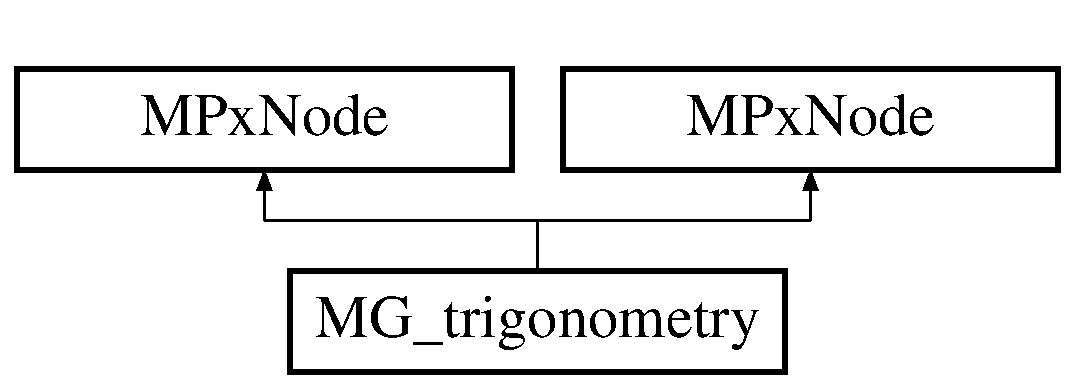
\includegraphics[height=2.000000cm]{class_m_g__trigonometry}
\end{center}
\end{figure}
\subsection*{Public Member Functions}
\begin{DoxyCompactItemize}
\item 
\hypertarget{class_m_g__trigonometry_aced7068cd45cd709efa05a906f21c7ee}{virtual M\-Status {\bfseries compute} (const M\-Plug \&plug, M\-Data\-Block \&data)}\label{class_m_g__trigonometry_aced7068cd45cd709efa05a906f21c7ee}

\item 
\hypertarget{class_m_g__trigonometry_aced7068cd45cd709efa05a906f21c7ee}{virtual M\-Status {\bfseries compute} (const M\-Plug \&plug, M\-Data\-Block \&data)}\label{class_m_g__trigonometry_aced7068cd45cd709efa05a906f21c7ee}

\end{DoxyCompactItemize}
\subsection*{Static Public Member Functions}
\begin{DoxyCompactItemize}
\item 
\hypertarget{class_m_g__trigonometry_a9a9c9fff9bbf2ab1f34a781e3289a802}{static void $\ast$ {\bfseries creator} ()}\label{class_m_g__trigonometry_a9a9c9fff9bbf2ab1f34a781e3289a802}

\item 
\hypertarget{class_m_g__trigonometry_a765dd745568862107f923765ebaf6f74}{static M\-Status {\bfseries initialize} ()}\label{class_m_g__trigonometry_a765dd745568862107f923765ebaf6f74}

\item 
\hypertarget{class_m_g__trigonometry_a9a9c9fff9bbf2ab1f34a781e3289a802}{static void $\ast$ {\bfseries creator} ()}\label{class_m_g__trigonometry_a9a9c9fff9bbf2ab1f34a781e3289a802}

\item 
\hypertarget{class_m_g__trigonometry_a765dd745568862107f923765ebaf6f74}{static M\-Status {\bfseries initialize} ()}\label{class_m_g__trigonometry_a765dd745568862107f923765ebaf6f74}

\end{DoxyCompactItemize}
\subsection*{Static Public Attributes}
\begin{DoxyCompactItemize}
\item 
static M\-Type\-Id \hyperlink{class_m_g__trigonometry_a9d74e233bd966adb8c060c4aae7a6576}{type\-Id}
\item 
static M\-Object \hyperlink{class_m_g__trigonometry_adf95381a397ca646e37a524dd4bae7fb}{input}
\item 
static M\-Object \hyperlink{class_m_g__trigonometry_a6be2c3fb2cfe5e7609eef7cd52802d6b}{math\-Operation}
\item 
static M\-Object \hyperlink{class_m_g__trigonometry_a92903c06ebef107b71b93812c7c358e3}{inverse\-Function}
\item 
static M\-Object \hyperlink{class_m_g__trigonometry_adde1f2175ff171bb94b96d6c3273f180}{output\-Value}
\end{DoxyCompactItemize}


\subsection{Detailed Description}
let s you perform some trigonometry operations 

\begin{DoxyAuthor}{Author}
Marco Giordano 
\end{DoxyAuthor}
\begin{DoxyDate}{Date}
--/--/2011 
\end{DoxyDate}
\begin{DoxyVersion}{Version}
latest version \-: V1 

changeload versions \-: \par
 V1 \-: \par

\begin{DoxyItemize}
\item initial release \par

\end{DoxyItemize}
\end{DoxyVersion}
node name \-: rivet\-Node.

details \-: This node let s you perform various trigonometry operations Just need to plug the input value and chose which operation to do.

example create node \-: (M\-E\-L) create\-Node \hyperlink{class_m_g__trigonometry}{M\-G\-\_\-trigonometry}. 

\subsection{Member Data Documentation}
\hypertarget{class_m_g__trigonometry_adf95381a397ca646e37a524dd4bae7fb}{\index{M\-G\-\_\-trigonometry@{M\-G\-\_\-trigonometry}!input@{input}}
\index{input@{input}!MG_trigonometry@{M\-G\-\_\-trigonometry}}
\subsubsection[{input}]{\setlength{\rightskip}{0pt plus 5cm}static M\-Object M\-G\-\_\-trigonometry\-::input\hspace{0.3cm}{\ttfamily [static]}}}\label{class_m_g__trigonometry_adf95381a397ca646e37a524dd4bae7fb}
This is the input value \hypertarget{class_m_g__trigonometry_a92903c06ebef107b71b93812c7c358e3}{\index{M\-G\-\_\-trigonometry@{M\-G\-\_\-trigonometry}!inverse\-Function@{inverse\-Function}}
\index{inverse\-Function@{inverse\-Function}!MG_trigonometry@{M\-G\-\_\-trigonometry}}
\subsubsection[{inverse\-Function}]{\setlength{\rightskip}{0pt plus 5cm}static M\-Object M\-G\-\_\-trigonometry\-::inverse\-Function\hspace{0.3cm}{\ttfamily [static]}}}\label{class_m_g__trigonometry_a92903c06ebef107b71b93812c7c358e3}
This attribute sets if to perform the inverse operation of the one set in the math\-Operation attribute \hypertarget{class_m_g__trigonometry_a6be2c3fb2cfe5e7609eef7cd52802d6b}{\index{M\-G\-\_\-trigonometry@{M\-G\-\_\-trigonometry}!math\-Operation@{math\-Operation}}
\index{math\-Operation@{math\-Operation}!MG_trigonometry@{M\-G\-\_\-trigonometry}}
\subsubsection[{math\-Operation}]{\setlength{\rightskip}{0pt plus 5cm}static M\-Object M\-G\-\_\-trigonometry\-::math\-Operation\hspace{0.3cm}{\ttfamily [static]}}}\label{class_m_g__trigonometry_a6be2c3fb2cfe5e7609eef7cd52802d6b}
This attribute sets the operation to perform \hypertarget{class_m_g__trigonometry_adde1f2175ff171bb94b96d6c3273f180}{\index{M\-G\-\_\-trigonometry@{M\-G\-\_\-trigonometry}!output\-Value@{output\-Value}}
\index{output\-Value@{output\-Value}!MG_trigonometry@{M\-G\-\_\-trigonometry}}
\subsubsection[{output\-Value}]{\setlength{\rightskip}{0pt plus 5cm}static M\-Object M\-G\-\_\-trigonometry\-::output\-Value\hspace{0.3cm}{\ttfamily [static]}}}\label{class_m_g__trigonometry_adde1f2175ff171bb94b96d6c3273f180}
This is the output attribute holding the computed data \hypertarget{class_m_g__trigonometry_a9d74e233bd966adb8c060c4aae7a6576}{\index{M\-G\-\_\-trigonometry@{M\-G\-\_\-trigonometry}!type\-Id@{type\-Id}}
\index{type\-Id@{type\-Id}!MG_trigonometry@{M\-G\-\_\-trigonometry}}
\subsubsection[{type\-Id}]{\setlength{\rightskip}{0pt plus 5cm}static M\-Type\-Id M\-G\-\_\-trigonometry\-::type\-Id\hspace{0.3cm}{\ttfamily [static]}}}\label{class_m_g__trigonometry_a9d74e233bd966adb8c060c4aae7a6576}
The node id 

The documentation for this class was generated from the following files\-:\begin{DoxyCompactItemize}
\item 
C\-:/\-Users/giordi/\-Desktop/\-P\-R\-O\-G\-E\-T\-T\-I\-\_\-\-I\-N\-\_\-\-C\-O\-R\-S\-O/\-C/\-M\-G\-\_\-\-Tools/cpp/\-M\-G\-\_\-tools\-Lite/src/M\-G\-\_\-trigonometry.\-h\item 
C\-:/\-Users/giordi/\-Desktop/\-P\-R\-O\-G\-E\-T\-T\-I\-\_\-\-I\-N\-\_\-\-C\-O\-R\-S\-O/\-C/\-M\-G\-\_\-\-Tools/cpp/\-M\-G\-\_\-trigonometry/src/M\-G\-\_\-trigonometry.\-h\end{DoxyCompactItemize}

\hypertarget{class_m_g__twist}{\section{M\-G\-\_\-twist Class Reference}
\label{class_m_g__twist}\index{M\-G\-\_\-twist@{M\-G\-\_\-twist}}
}


lets you extract a twist value from two transforms  




{\ttfamily \#include $<$M\-G\-\_\-twist.\-h$>$}

Inheritance diagram for M\-G\-\_\-twist\-:\begin{figure}[H]
\begin{center}
\leavevmode
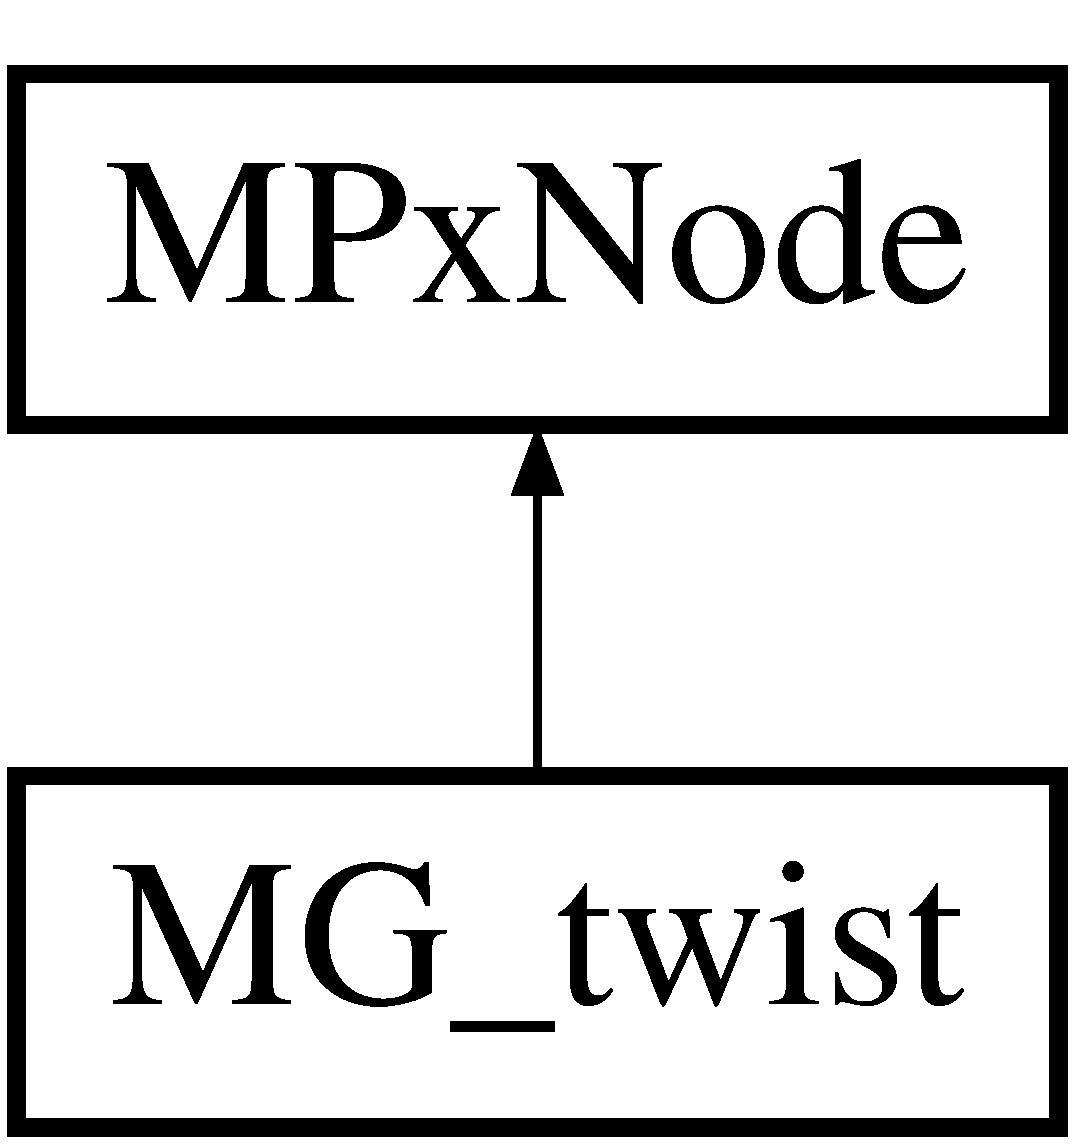
\includegraphics[height=2.000000cm]{class_m_g__twist}
\end{center}
\end{figure}
\subsection*{Public Member Functions}
\begin{DoxyCompactItemize}
\item 
\hypertarget{class_m_g__twist_ac9b4a271cdca26dc4ca7fb6eb56e390c}{virtual M\-Status {\bfseries compute} (const M\-Plug \&plug, M\-Data\-Block \&data\-Block)}\label{class_m_g__twist_ac9b4a271cdca26dc4ca7fb6eb56e390c}

\end{DoxyCompactItemize}
\subsection*{Static Public Member Functions}
\begin{DoxyCompactItemize}
\item 
\hypertarget{class_m_g__twist_a028726ad6a2ddbf567019014fd234b28}{static void $\ast$ {\bfseries creator} ()}\label{class_m_g__twist_a028726ad6a2ddbf567019014fd234b28}

\item 
\hypertarget{class_m_g__twist_a7d33df78fd5b162dc731a2668455f64c}{static M\-Status {\bfseries initialize} ()}\label{class_m_g__twist_a7d33df78fd5b162dc731a2668455f64c}

\end{DoxyCompactItemize}
\subsection*{Static Public Attributes}
\begin{DoxyCompactItemize}
\item 
static M\-Object \hyperlink{class_m_g__twist_a1f56e50333669ce2a38f71e3226ab18e}{matrix1}
\item 
static M\-Object \hyperlink{class_m_g__twist_a529b723501fff0dd68b7062a8816195b}{matrix2}
\item 
static M\-Object \hyperlink{class_m_g__twist_a53c3b473d1227aec0ff7a13d7a2ea246}{number\-Of\-Outputs}
\item 
static M\-Object \hyperlink{class_m_g__twist_a8b36730a0d0d26103ebcd04b26479c23}{twist\-Axis}
\item 
static M\-Object \hyperlink{class_m_g__twist_a290ab074cc022d06d1498fa3a96e1d20}{output\-Translate\-X}
\item 
static M\-Object \hyperlink{class_m_g__twist_acf377991d45f3bda1fb51bc6509d6d81}{output\-Translate\-Y}
\item 
static M\-Object \hyperlink{class_m_g__twist_a4dda83e85c12b6a8b58775bf1b3d38bb}{output\-Translate\-Z}
\item 
static M\-Object \hyperlink{class_m_g__twist_a7e48847c5606a677f1dc1ea4bdb3402d}{output\-Translate}
\item 
static M\-Object \hyperlink{class_m_g__twist_a20fee814720fcaee9b09f7de20f0b286}{output\-Rotate\-X}
\item 
static M\-Object \hyperlink{class_m_g__twist_a37e96db269a8af41fe9f808a35d27967}{output\-Rotate\-Y}
\item 
static M\-Object \hyperlink{class_m_g__twist_a3cae9cd439fd68b38b77ae4e439f64d5}{output\-Rotate\-Z}
\item 
static M\-Object \hyperlink{class_m_g__twist_a3908aa57e152eb462614eefb56bb82fb}{output\-Rotate}
\item 
\hypertarget{class_m_g__twist_a79fb6cae99e39340484b4434f1fd9e70}{static M\-Type\-Id {\bfseries type\-Id}}\label{class_m_g__twist_a79fb6cae99e39340484b4434f1fd9e70}

\end{DoxyCompactItemize}


\subsection{Detailed Description}
lets you extract a twist value from two transforms 

\begin{DoxyAuthor}{Author}
Marco Giordano 
\end{DoxyAuthor}
\begin{DoxyDate}{Date}
1/24/2013 
\end{DoxyDate}
\begin{DoxyVersion}{Version}
latest version \-: V1 

changeload versions \-: \par
 V1 \-: \par

\begin{DoxyItemize}
\item initial release \par
 V2 \-: \par

\item implemented different twist axis rather then only Y \par
 node name \-: \hyperlink{class_m_g__twist}{M\-G\-\_\-twist}
\end{DoxyItemize}
\end{DoxyVersion}
details \-: This node lets you extract a twist value from two transforms

example create node \-: (M\-E\-L) create\-Node \hyperlink{class_m_g__twist}{M\-G\-\_\-twist}.

\begin{DoxyRefDesc}{Todo}
\item[\hyperlink{todo__todo000010}{Todo}]set output data with a single array data builder rather then one at the time in order to improve performances 

implement more type of distribuition for for the outputs\end{DoxyRefDesc}


\subsection{Member Data Documentation}
\hypertarget{class_m_g__twist_a1f56e50333669ce2a38f71e3226ab18e}{\index{M\-G\-\_\-twist@{M\-G\-\_\-twist}!matrix1@{matrix1}}
\index{matrix1@{matrix1}!MG_twist@{M\-G\-\_\-twist}}
\subsubsection[{matrix1}]{\setlength{\rightskip}{0pt plus 5cm}M\-Object M\-G\-\_\-twist\-::matrix1\hspace{0.3cm}{\ttfamily [static]}}}\label{class_m_g__twist_a1f56e50333669ce2a38f71e3226ab18e}
The first matrix to calculate the twist from \hypertarget{class_m_g__twist_a529b723501fff0dd68b7062a8816195b}{\index{M\-G\-\_\-twist@{M\-G\-\_\-twist}!matrix2@{matrix2}}
\index{matrix2@{matrix2}!MG_twist@{M\-G\-\_\-twist}}
\subsubsection[{matrix2}]{\setlength{\rightskip}{0pt plus 5cm}M\-Object M\-G\-\_\-twist\-::matrix2\hspace{0.3cm}{\ttfamily [static]}}}\label{class_m_g__twist_a529b723501fff0dd68b7062a8816195b}
The second matrix to calculate the twist from \hypertarget{class_m_g__twist_a53c3b473d1227aec0ff7a13d7a2ea246}{\index{M\-G\-\_\-twist@{M\-G\-\_\-twist}!number\-Of\-Outputs@{number\-Of\-Outputs}}
\index{number\-Of\-Outputs@{number\-Of\-Outputs}!MG_twist@{M\-G\-\_\-twist}}
\subsubsection[{number\-Of\-Outputs}]{\setlength{\rightskip}{0pt plus 5cm}M\-Object M\-G\-\_\-twist\-::number\-Of\-Outputs\hspace{0.3cm}{\ttfamily [static]}}}\label{class_m_g__twist_a53c3b473d1227aec0ff7a13d7a2ea246}
How many output twist will be computed \hypertarget{class_m_g__twist_a3908aa57e152eb462614eefb56bb82fb}{\index{M\-G\-\_\-twist@{M\-G\-\_\-twist}!output\-Rotate@{output\-Rotate}}
\index{output\-Rotate@{output\-Rotate}!MG_twist@{M\-G\-\_\-twist}}
\subsubsection[{output\-Rotate}]{\setlength{\rightskip}{0pt plus 5cm}M\-Object M\-G\-\_\-twist\-::output\-Rotate\hspace{0.3cm}{\ttfamily [static]}}}\label{class_m_g__twist_a3908aa57e152eb462614eefb56bb82fb}
This is the output Rotate array \hypertarget{class_m_g__twist_a20fee814720fcaee9b09f7de20f0b286}{\index{M\-G\-\_\-twist@{M\-G\-\_\-twist}!output\-Rotate\-X@{output\-Rotate\-X}}
\index{output\-Rotate\-X@{output\-Rotate\-X}!MG_twist@{M\-G\-\_\-twist}}
\subsubsection[{output\-Rotate\-X}]{\setlength{\rightskip}{0pt plus 5cm}M\-Object M\-G\-\_\-twist\-::output\-Rotate\-X\hspace{0.3cm}{\ttfamily [static]}}}\label{class_m_g__twist_a20fee814720fcaee9b09f7de20f0b286}
This is the X component of the output Rotate array \hypertarget{class_m_g__twist_a37e96db269a8af41fe9f808a35d27967}{\index{M\-G\-\_\-twist@{M\-G\-\_\-twist}!output\-Rotate\-Y@{output\-Rotate\-Y}}
\index{output\-Rotate\-Y@{output\-Rotate\-Y}!MG_twist@{M\-G\-\_\-twist}}
\subsubsection[{output\-Rotate\-Y}]{\setlength{\rightskip}{0pt plus 5cm}M\-Object M\-G\-\_\-twist\-::output\-Rotate\-Y\hspace{0.3cm}{\ttfamily [static]}}}\label{class_m_g__twist_a37e96db269a8af41fe9f808a35d27967}
This is the Y component of the output Rotate array \hypertarget{class_m_g__twist_a3cae9cd439fd68b38b77ae4e439f64d5}{\index{M\-G\-\_\-twist@{M\-G\-\_\-twist}!output\-Rotate\-Z@{output\-Rotate\-Z}}
\index{output\-Rotate\-Z@{output\-Rotate\-Z}!MG_twist@{M\-G\-\_\-twist}}
\subsubsection[{output\-Rotate\-Z}]{\setlength{\rightskip}{0pt plus 5cm}M\-Object M\-G\-\_\-twist\-::output\-Rotate\-Z\hspace{0.3cm}{\ttfamily [static]}}}\label{class_m_g__twist_a3cae9cd439fd68b38b77ae4e439f64d5}
This is the Z component of the output Rotate array \hypertarget{class_m_g__twist_a7e48847c5606a677f1dc1ea4bdb3402d}{\index{M\-G\-\_\-twist@{M\-G\-\_\-twist}!output\-Translate@{output\-Translate}}
\index{output\-Translate@{output\-Translate}!MG_twist@{M\-G\-\_\-twist}}
\subsubsection[{output\-Translate}]{\setlength{\rightskip}{0pt plus 5cm}M\-Object M\-G\-\_\-twist\-::output\-Translate\hspace{0.3cm}{\ttfamily [static]}}}\label{class_m_g__twist_a7e48847c5606a677f1dc1ea4bdb3402d}
This is the output translate array \hypertarget{class_m_g__twist_a290ab074cc022d06d1498fa3a96e1d20}{\index{M\-G\-\_\-twist@{M\-G\-\_\-twist}!output\-Translate\-X@{output\-Translate\-X}}
\index{output\-Translate\-X@{output\-Translate\-X}!MG_twist@{M\-G\-\_\-twist}}
\subsubsection[{output\-Translate\-X}]{\setlength{\rightskip}{0pt plus 5cm}M\-Object M\-G\-\_\-twist\-::output\-Translate\-X\hspace{0.3cm}{\ttfamily [static]}}}\label{class_m_g__twist_a290ab074cc022d06d1498fa3a96e1d20}
This is the X component of the output translate array \hypertarget{class_m_g__twist_acf377991d45f3bda1fb51bc6509d6d81}{\index{M\-G\-\_\-twist@{M\-G\-\_\-twist}!output\-Translate\-Y@{output\-Translate\-Y}}
\index{output\-Translate\-Y@{output\-Translate\-Y}!MG_twist@{M\-G\-\_\-twist}}
\subsubsection[{output\-Translate\-Y}]{\setlength{\rightskip}{0pt plus 5cm}M\-Object M\-G\-\_\-twist\-::output\-Translate\-Y\hspace{0.3cm}{\ttfamily [static]}}}\label{class_m_g__twist_acf377991d45f3bda1fb51bc6509d6d81}
This is the Y component of the output translate array \hypertarget{class_m_g__twist_a4dda83e85c12b6a8b58775bf1b3d38bb}{\index{M\-G\-\_\-twist@{M\-G\-\_\-twist}!output\-Translate\-Z@{output\-Translate\-Z}}
\index{output\-Translate\-Z@{output\-Translate\-Z}!MG_twist@{M\-G\-\_\-twist}}
\subsubsection[{output\-Translate\-Z}]{\setlength{\rightskip}{0pt plus 5cm}M\-Object M\-G\-\_\-twist\-::output\-Translate\-Z\hspace{0.3cm}{\ttfamily [static]}}}\label{class_m_g__twist_a4dda83e85c12b6a8b58775bf1b3d38bb}
This is the Z component of the output translate array \hypertarget{class_m_g__twist_a8b36730a0d0d26103ebcd04b26479c23}{\index{M\-G\-\_\-twist@{M\-G\-\_\-twist}!twist\-Axis@{twist\-Axis}}
\index{twist\-Axis@{twist\-Axis}!MG_twist@{M\-G\-\_\-twist}}
\subsubsection[{twist\-Axis}]{\setlength{\rightskip}{0pt plus 5cm}M\-Object M\-G\-\_\-twist\-::twist\-Axis\hspace{0.3cm}{\ttfamily [static]}}}\label{class_m_g__twist_a8b36730a0d0d26103ebcd04b26479c23}
This is the axis that will be used for computation 

The documentation for this class was generated from the following file\-:\begin{DoxyCompactItemize}
\item 
C\-:/\-Users/giordi/\-Desktop/\-P\-R\-O\-G\-E\-T\-T\-I\-\_\-\-I\-N\-\_\-\-C\-O\-R\-S\-O/\-C/\-M\-G\-\_\-\-Tools/cpp/\-M\-G\-\_\-twist/src/M\-G\-\_\-twist.\-h\end{DoxyCompactItemize}

\hypertarget{class_m_g__vector}{\section{M\-G\-\_\-vector Class Reference}
\label{class_m_g__vector}\index{M\-G\-\_\-vector@{M\-G\-\_\-vector}}
}


lets you quickly create a vector  




{\ttfamily \#include $<$M\-G\-\_\-vector.\-h$>$}

Inheritance diagram for M\-G\-\_\-vector\-:\begin{figure}[H]
\begin{center}
\leavevmode
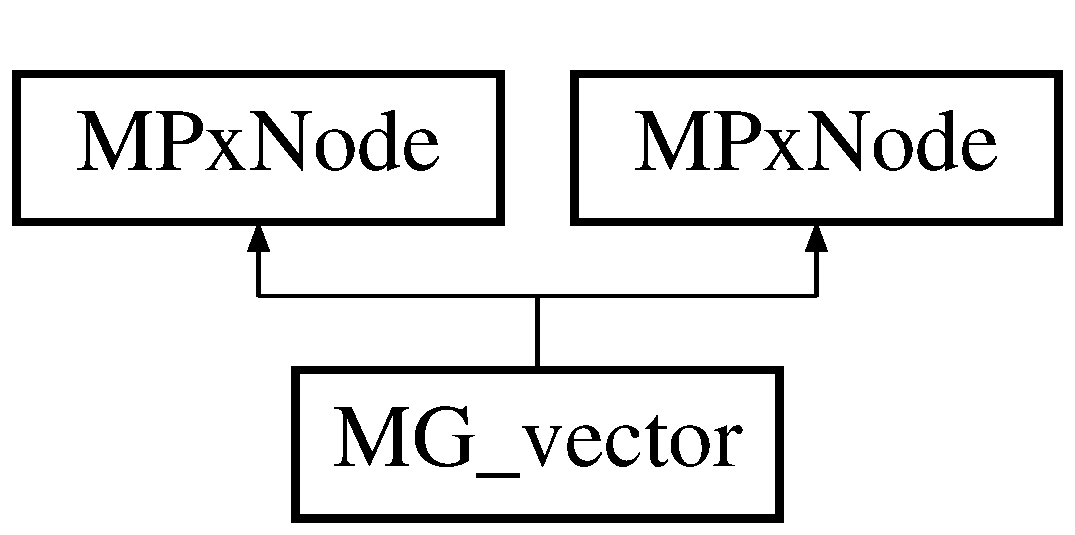
\includegraphics[height=2.000000cm]{class_m_g__vector}
\end{center}
\end{figure}
\subsection*{Public Member Functions}
\begin{DoxyCompactItemize}
\item 
\hypertarget{class_m_g__vector_a8da2ac463306acc395900f2b5d2402d7}{virtual M\-Status {\bfseries compute} (const M\-Plug \&plug, M\-Data\-Block \&data\-Block)}\label{class_m_g__vector_a8da2ac463306acc395900f2b5d2402d7}

\item 
\hypertarget{class_m_g__vector_a8da2ac463306acc395900f2b5d2402d7}{virtual M\-Status {\bfseries compute} (const M\-Plug \&plug, M\-Data\-Block \&data\-Block)}\label{class_m_g__vector_a8da2ac463306acc395900f2b5d2402d7}

\end{DoxyCompactItemize}
\subsection*{Static Public Member Functions}
\begin{DoxyCompactItemize}
\item 
\hypertarget{class_m_g__vector_a4a84b7bfa0e06ce993b8b03d9a95c50c}{static void $\ast$ {\bfseries creator} ()}\label{class_m_g__vector_a4a84b7bfa0e06ce993b8b03d9a95c50c}

\item 
\hypertarget{class_m_g__vector_ab2703616d4245176896a792964f28982}{static M\-Status {\bfseries initialize} ()}\label{class_m_g__vector_ab2703616d4245176896a792964f28982}

\item 
\hypertarget{class_m_g__vector_a4a84b7bfa0e06ce993b8b03d9a95c50c}{static void $\ast$ {\bfseries creator} ()}\label{class_m_g__vector_a4a84b7bfa0e06ce993b8b03d9a95c50c}

\item 
\hypertarget{class_m_g__vector_ab2703616d4245176896a792964f28982}{static M\-Status {\bfseries initialize} ()}\label{class_m_g__vector_ab2703616d4245176896a792964f28982}

\end{DoxyCompactItemize}
\subsection*{Static Public Attributes}
\begin{DoxyCompactItemize}
\item 
static M\-Object \hyperlink{class_m_g__vector_a442ebd6c40bb57b043081c3feb80de8d}{input\-M1}
\item 
static M\-Object \hyperlink{class_m_g__vector_ad2068ee6d5828d8ef653b3b296d92dcc}{input\-M2}
\item 
static M\-Object \hyperlink{class_m_g__vector_a234df1cfa76968bc856b83c80b30f5d6}{magnitude}
\item 
static M\-Object \hyperlink{class_m_g__vector_ac3d4326cf87a24ff99a3a1e746997919}{o\-Vec\-X}
\item 
static M\-Object \hyperlink{class_m_g__vector_a8b7f9011aa8c58993f9946dfc4b539df}{o\-Vec\-Y}
\item 
static M\-Object \hyperlink{class_m_g__vector_adcfd5002d7260461ba813c5e77668022}{o\-Vec\-Z}
\item 
static M\-Object \hyperlink{class_m_g__vector_a8e3c1d4392648a517a240e749e4acfd4}{o\-Vec}
\item 
static M\-Object \hyperlink{class_m_g__vector_a0da85667dd839cd51882829a3c168a6c}{normalize}
\item 
static M\-Type\-Id \hyperlink{class_m_g__vector_ac4417888ca111086a0b3e5778041cb7e}{type\-Id}
\end{DoxyCompactItemize}


\subsection{Detailed Description}
lets you quickly create a vector 

\begin{DoxyAuthor}{Author}
Marco Giordano 
\end{DoxyAuthor}
\begin{DoxyDate}{Date}
--/--/2011 
\end{DoxyDate}
\begin{DoxyVersion}{Version}
latest version \-: V1 

changeload versions \-: \par
 V1 \-: \par

\begin{DoxyItemize}
\item initial release \par

\end{DoxyItemize}
\end{DoxyVersion}
node name \-: \hyperlink{class_m_g__vector}{M\-G\-\_\-vector}.

details \-: This node lets you quickly create a vector This node from two matrices generates a vector and calculates its magnitude, also provide an attribute to normalize the output vector if needed

example create node \-: (M\-E\-L) create\-Node \hyperlink{class_m_g__vector}{M\-G\-\_\-vector}.

\begin{DoxyRefDesc}{Todo}
\item[\hyperlink{todo__todo000011}{Todo}]convert the node to a locator and addoption to draw the vector\end{DoxyRefDesc}


\begin{DoxyAuthor}{Author}
Marco Giordano 
\end{DoxyAuthor}
\begin{DoxyDate}{Date}
--/--/2011 
\end{DoxyDate}
\begin{DoxyVersion}{Version}
latest version \-: V1 

changeload versions \-: \par
 V1 \-: \par

\begin{DoxyItemize}
\item initial release \par

\end{DoxyItemize}
\end{DoxyVersion}
node name \-: \hyperlink{class_m_g__vector}{M\-G\-\_\-vector}.

details \-: This node lets you quickly create a vector This node from two matrices generates a vector and calculates its magnitude, also provide an attribute to normalize the output vector if needed

example create node \-: (M\-E\-L) create\-Node \hyperlink{class_m_g__vector}{M\-G\-\_\-vector}.

\begin{DoxyRefDesc}{Todo}
\item[\hyperlink{todo__todo000012}{Todo}]convert the node to a locator and addoption to draw the vector\end{DoxyRefDesc}


\subsection{Member Data Documentation}
\hypertarget{class_m_g__vector_a442ebd6c40bb57b043081c3feb80de8d}{\index{M\-G\-\_\-vector@{M\-G\-\_\-vector}!input\-M1@{input\-M1}}
\index{input\-M1@{input\-M1}!MG_vector@{M\-G\-\_\-vector}}
\subsubsection[{input\-M1}]{\setlength{\rightskip}{0pt plus 5cm}static M\-Object M\-G\-\_\-vector\-::input\-M1\hspace{0.3cm}{\ttfamily [static]}}}\label{class_m_g__vector_a442ebd6c40bb57b043081c3feb80de8d}
The first input matrix attribute \hypertarget{class_m_g__vector_ad2068ee6d5828d8ef653b3b296d92dcc}{\index{M\-G\-\_\-vector@{M\-G\-\_\-vector}!input\-M2@{input\-M2}}
\index{input\-M2@{input\-M2}!MG_vector@{M\-G\-\_\-vector}}
\subsubsection[{input\-M2}]{\setlength{\rightskip}{0pt plus 5cm}static M\-Object M\-G\-\_\-vector\-::input\-M2\hspace{0.3cm}{\ttfamily [static]}}}\label{class_m_g__vector_ad2068ee6d5828d8ef653b3b296d92dcc}
The second input matrix attribute \hypertarget{class_m_g__vector_a234df1cfa76968bc856b83c80b30f5d6}{\index{M\-G\-\_\-vector@{M\-G\-\_\-vector}!magnitude@{magnitude}}
\index{magnitude@{magnitude}!MG_vector@{M\-G\-\_\-vector}}
\subsubsection[{magnitude}]{\setlength{\rightskip}{0pt plus 5cm}static M\-Object M\-G\-\_\-vector\-::magnitude\hspace{0.3cm}{\ttfamily [static]}}}\label{class_m_g__vector_a234df1cfa76968bc856b83c80b30f5d6}
This attribute holds the length of the vector \hypertarget{class_m_g__vector_a0da85667dd839cd51882829a3c168a6c}{\index{M\-G\-\_\-vector@{M\-G\-\_\-vector}!normalize@{normalize}}
\index{normalize@{normalize}!MG_vector@{M\-G\-\_\-vector}}
\subsubsection[{normalize}]{\setlength{\rightskip}{0pt plus 5cm}static M\-Object M\-G\-\_\-vector\-::normalize\hspace{0.3cm}{\ttfamily [static]}}}\label{class_m_g__vector_a0da85667dd839cd51882829a3c168a6c}
This attribute if checked normalize the output vector \hypertarget{class_m_g__vector_a8e3c1d4392648a517a240e749e4acfd4}{\index{M\-G\-\_\-vector@{M\-G\-\_\-vector}!o\-Vec@{o\-Vec}}
\index{o\-Vec@{o\-Vec}!MG_vector@{M\-G\-\_\-vector}}
\subsubsection[{o\-Vec}]{\setlength{\rightskip}{0pt plus 5cm}static M\-Object M\-G\-\_\-vector\-::o\-Vec\hspace{0.3cm}{\ttfamily [static]}}}\label{class_m_g__vector_a8e3c1d4392648a517a240e749e4acfd4}
The output vector attribute \hypertarget{class_m_g__vector_ac3d4326cf87a24ff99a3a1e746997919}{\index{M\-G\-\_\-vector@{M\-G\-\_\-vector}!o\-Vec\-X@{o\-Vec\-X}}
\index{o\-Vec\-X@{o\-Vec\-X}!MG_vector@{M\-G\-\_\-vector}}
\subsubsection[{o\-Vec\-X}]{\setlength{\rightskip}{0pt plus 5cm}static M\-Object M\-G\-\_\-vector\-::o\-Vec\-X\hspace{0.3cm}{\ttfamily [static]}}}\label{class_m_g__vector_ac3d4326cf87a24ff99a3a1e746997919}
The X component of the output vector attribute \hypertarget{class_m_g__vector_a8b7f9011aa8c58993f9946dfc4b539df}{\index{M\-G\-\_\-vector@{M\-G\-\_\-vector}!o\-Vec\-Y@{o\-Vec\-Y}}
\index{o\-Vec\-Y@{o\-Vec\-Y}!MG_vector@{M\-G\-\_\-vector}}
\subsubsection[{o\-Vec\-Y}]{\setlength{\rightskip}{0pt plus 5cm}static M\-Object M\-G\-\_\-vector\-::o\-Vec\-Y\hspace{0.3cm}{\ttfamily [static]}}}\label{class_m_g__vector_a8b7f9011aa8c58993f9946dfc4b539df}
The Y component of the output vector attribute \hypertarget{class_m_g__vector_adcfd5002d7260461ba813c5e77668022}{\index{M\-G\-\_\-vector@{M\-G\-\_\-vector}!o\-Vec\-Z@{o\-Vec\-Z}}
\index{o\-Vec\-Z@{o\-Vec\-Z}!MG_vector@{M\-G\-\_\-vector}}
\subsubsection[{o\-Vec\-Z}]{\setlength{\rightskip}{0pt plus 5cm}static M\-Object M\-G\-\_\-vector\-::o\-Vec\-Z\hspace{0.3cm}{\ttfamily [static]}}}\label{class_m_g__vector_adcfd5002d7260461ba813c5e77668022}
The Z component of the output vector attribute \hypertarget{class_m_g__vector_ac4417888ca111086a0b3e5778041cb7e}{\index{M\-G\-\_\-vector@{M\-G\-\_\-vector}!type\-Id@{type\-Id}}
\index{type\-Id@{type\-Id}!MG_vector@{M\-G\-\_\-vector}}
\subsubsection[{type\-Id}]{\setlength{\rightskip}{0pt plus 5cm}static M\-Type\-Id M\-G\-\_\-vector\-::type\-Id\hspace{0.3cm}{\ttfamily [static]}}}\label{class_m_g__vector_ac4417888ca111086a0b3e5778041cb7e}
The node id 

The documentation for this class was generated from the following files\-:\begin{DoxyCompactItemize}
\item 
C\-:/\-Users/giordi/\-Desktop/\-P\-R\-O\-G\-E\-T\-T\-I\-\_\-\-I\-N\-\_\-\-C\-O\-R\-S\-O/\-C/\-M\-G\-\_\-\-Tools/cpp/\-M\-G\-\_\-tools\-Lite/src/M\-G\-\_\-vector.\-h\item 
C\-:/\-Users/giordi/\-Desktop/\-P\-R\-O\-G\-E\-T\-T\-I\-\_\-\-I\-N\-\_\-\-C\-O\-R\-S\-O/\-C/\-M\-G\-\_\-\-Tools/cpp/\-M\-G\-\_\-vector/src/M\-G\-\_\-vector.\-h\end{DoxyCompactItemize}

\hypertarget{class_m_g__vector_g_l}{\section{M\-G\-\_\-vector\-G\-L Class Reference}
\label{class_m_g__vector_g_l}\index{M\-G\-\_\-vector\-G\-L@{M\-G\-\_\-vector\-G\-L}}
}


let s you draw an array of vectors in maya viewport  




{\ttfamily \#include $<$M\-G\-\_\-vector\-G\-L.\-h$>$}

Inheritance diagram for M\-G\-\_\-vector\-G\-L\-:\begin{figure}[H]
\begin{center}
\leavevmode
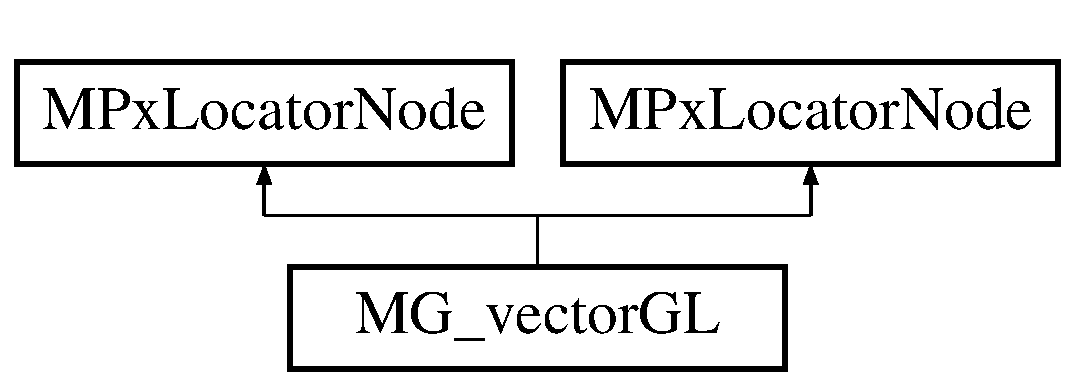
\includegraphics[height=2.000000cm]{class_m_g__vector_g_l}
\end{center}
\end{figure}
\subsection*{Public Member Functions}
\begin{DoxyCompactItemize}
\item 
\hypertarget{class_m_g__vector_g_l_ab1e2e5081a30bbf5dce3e0b010990719}{virtual M\-Status {\bfseries compute} (const M\-Plug \&plug, M\-Data\-Block \&data)}\label{class_m_g__vector_g_l_ab1e2e5081a30bbf5dce3e0b010990719}

\item 
\hypertarget{class_m_g__vector_g_l_adef6c3a74ae350ef344956af36953347}{virtual void {\bfseries draw} (M3d\-View \&, const M\-Dag\-Path \&, M3d\-View\-::\-Display\-Style, M3d\-View\-::\-Display\-Status)}\label{class_m_g__vector_g_l_adef6c3a74ae350ef344956af36953347}

\item 
\hypertarget{class_m_g__vector_g_l_afceff90a8f00ef5f68c2b41032e0a3ec}{virtual bool {\bfseries is\-Bounded} () const }\label{class_m_g__vector_g_l_afceff90a8f00ef5f68c2b41032e0a3ec}

\item 
\hypertarget{class_m_g__vector_g_l_ab1e2e5081a30bbf5dce3e0b010990719}{virtual M\-Status {\bfseries compute} (const M\-Plug \&plug, M\-Data\-Block \&data)}\label{class_m_g__vector_g_l_ab1e2e5081a30bbf5dce3e0b010990719}

\item 
\hypertarget{class_m_g__vector_g_l_adef6c3a74ae350ef344956af36953347}{virtual void {\bfseries draw} (M3d\-View \&, const M\-Dag\-Path \&, M3d\-View\-::\-Display\-Style, M3d\-View\-::\-Display\-Status)}\label{class_m_g__vector_g_l_adef6c3a74ae350ef344956af36953347}

\item 
\hypertarget{class_m_g__vector_g_l_afceff90a8f00ef5f68c2b41032e0a3ec}{virtual bool {\bfseries is\-Bounded} () const }\label{class_m_g__vector_g_l_afceff90a8f00ef5f68c2b41032e0a3ec}

\end{DoxyCompactItemize}
\subsection*{Static Public Member Functions}
\begin{DoxyCompactItemize}
\item 
\hypertarget{class_m_g__vector_g_l_ab624fc88b122ddaf90df3c8e20a91eae}{static void $\ast$ {\bfseries creator} ()}\label{class_m_g__vector_g_l_ab624fc88b122ddaf90df3c8e20a91eae}

\item 
\hypertarget{class_m_g__vector_g_l_aeed920d819de46588bc75ca4c77f957b}{static M\-Status {\bfseries initialize} ()}\label{class_m_g__vector_g_l_aeed920d819de46588bc75ca4c77f957b}

\item 
\hypertarget{class_m_g__vector_g_l_ab624fc88b122ddaf90df3c8e20a91eae}{static void $\ast$ {\bfseries creator} ()}\label{class_m_g__vector_g_l_ab624fc88b122ddaf90df3c8e20a91eae}

\item 
\hypertarget{class_m_g__vector_g_l_aeed920d819de46588bc75ca4c77f957b}{static M\-Status {\bfseries initialize} ()}\label{class_m_g__vector_g_l_aeed920d819de46588bc75ca4c77f957b}

\end{DoxyCompactItemize}
\subsection*{Static Public Attributes}
\begin{DoxyCompactItemize}
\item 
static M\-Type\-Id \hyperlink{class_m_g__vector_g_l_acca8150a834863494fd5f1b00680289e}{type\-Id}
\item 
static M\-Object \hyperlink{class_m_g__vector_g_l_a70c7ff57dc885d2fed64e61fa6dce7c4}{up\-Vec\-X}
\item 
static M\-Object \hyperlink{class_m_g__vector_g_l_abccaa6f4f93a98f68c0aec200763f6c5}{up\-Vec\-Y}
\item 
static M\-Object \hyperlink{class_m_g__vector_g_l_aa5348daa3385f54237190545cdf21009}{up\-Vec\-Z}
\item 
static M\-Object \hyperlink{class_m_g__vector_g_l_a9fa637bb5b24532d768f5b8912c3f92e}{up\-Vec}
\item 
static M\-Object \hyperlink{class_m_g__vector_g_l_ae7c3a0612e7db7b56e6e96c0179aefc6}{start\-Point\-X}
\item 
static M\-Object \hyperlink{class_m_g__vector_g_l_af1d06d50730959946fc5db507eefa3aa}{start\-Point\-Y}
\item 
static M\-Object \hyperlink{class_m_g__vector_g_l_a00e63c6a4cf63e7c71cc22e094578470}{start\-Point\-Z}
\item 
static M\-Object \hyperlink{class_m_g__vector_g_l_ac0ca586f36cae208f5fb0655d5f5a534}{start\-Point}
\item 
static M\-Object \hyperlink{class_m_g__vector_g_l_ac9e29eb01772ab64b67fe0ac130dceef}{fake\-Out}
\item 
static M\-Object \hyperlink{class_m_g__vector_g_l_a6eeaca2cfdf01a1cde7727a7d02e9fb8}{vec\-X}
\item 
static M\-Object \hyperlink{class_m_g__vector_g_l_ab83a515ef8a0389db4fffdd27deb0a15}{vec\-Y}
\item 
static M\-Object \hyperlink{class_m_g__vector_g_l_a793496afb749c8d022fb487e7cb7ef50}{vec\-Z}
\item 
static M\-Object \hyperlink{class_m_g__vector_g_l_a7e8fcd12774565e52cfc9a088426fda5}{vecs}
\item 
static M\-Object \hyperlink{class_m_g__vector_g_l_a5d59b4c3dfc50250558acfabca45a260}{draw\-It}
\item 
static M\-Object \hyperlink{class_m_g__vector_g_l_a51ce57b6d4cac43cf6b9fbdf377691c4}{arrow\-Size}
\end{DoxyCompactItemize}


\subsection{Detailed Description}
let s you draw an array of vectors in maya viewport 

\begin{DoxyAuthor}{Author}
Marco Giordano 
\end{DoxyAuthor}
\begin{DoxyDate}{Date}
02/11/2013 
\end{DoxyDate}
\begin{DoxyVersion}{Version}
latest version \-: V1 

changeload versions \-: \par
 V1 \-: \par

\begin{DoxyItemize}
\item initial release \par

\end{DoxyItemize}
\end{DoxyVersion}
node name \-: \hyperlink{class_m_g__vector_g_l}{M\-G\-\_\-vector\-G\-L}.

details \-: This nodelet s you draw an array of vectors in maya viewport. This node is used for debugging purpose , connect in the vecs attribute all the vectors you want to draw and in the start\-Poits array all the base positions for the vectors, connect the fake out attribute to something in order to force the compute

example create node \-: (M\-E\-L) create\-Node \hyperlink{class_m_g__vector_g_l}{M\-G\-\_\-vector\-G\-L}. 

\subsection{Member Data Documentation}
\hypertarget{class_m_g__vector_g_l_a51ce57b6d4cac43cf6b9fbdf377691c4}{\index{M\-G\-\_\-vector\-G\-L@{M\-G\-\_\-vector\-G\-L}!arrow\-Size@{arrow\-Size}}
\index{arrow\-Size@{arrow\-Size}!MG_vectorGL@{M\-G\-\_\-vector\-G\-L}}
\subsubsection[{arrow\-Size}]{\setlength{\rightskip}{0pt plus 5cm}static M\-Object M\-G\-\_\-vector\-G\-L\-::arrow\-Size\hspace{0.3cm}{\ttfamily [static]}}}\label{class_m_g__vector_g_l_a51ce57b6d4cac43cf6b9fbdf377691c4}
This attribute sets the arrow size \hypertarget{class_m_g__vector_g_l_a5d59b4c3dfc50250558acfabca45a260}{\index{M\-G\-\_\-vector\-G\-L@{M\-G\-\_\-vector\-G\-L}!draw\-It@{draw\-It}}
\index{draw\-It@{draw\-It}!MG_vectorGL@{M\-G\-\_\-vector\-G\-L}}
\subsubsection[{draw\-It}]{\setlength{\rightskip}{0pt plus 5cm}static M\-Object M\-G\-\_\-vector\-G\-L\-::draw\-It\hspace{0.3cm}{\ttfamily [static]}}}\label{class_m_g__vector_g_l_a5d59b4c3dfc50250558acfabca45a260}
This attribute sets whether or not to draw the arrows \hypertarget{class_m_g__vector_g_l_ac9e29eb01772ab64b67fe0ac130dceef}{\index{M\-G\-\_\-vector\-G\-L@{M\-G\-\_\-vector\-G\-L}!fake\-Out@{fake\-Out}}
\index{fake\-Out@{fake\-Out}!MG_vectorGL@{M\-G\-\_\-vector\-G\-L}}
\subsubsection[{fake\-Out}]{\setlength{\rightskip}{0pt plus 5cm}static M\-Object M\-G\-\_\-vector\-G\-L\-::fake\-Out\hspace{0.3cm}{\ttfamily [static]}}}\label{class_m_g__vector_g_l_ac9e29eb01772ab64b67fe0ac130dceef}
The fake attribute used to force the compute to evaluate \hypertarget{class_m_g__vector_g_l_ac0ca586f36cae208f5fb0655d5f5a534}{\index{M\-G\-\_\-vector\-G\-L@{M\-G\-\_\-vector\-G\-L}!start\-Point@{start\-Point}}
\index{start\-Point@{start\-Point}!MG_vectorGL@{M\-G\-\_\-vector\-G\-L}}
\subsubsection[{start\-Point}]{\setlength{\rightskip}{0pt plus 5cm}static M\-Object M\-G\-\_\-vector\-G\-L\-::start\-Point\hspace{0.3cm}{\ttfamily [static]}}}\label{class_m_g__vector_g_l_ac0ca586f36cae208f5fb0655d5f5a534}
The the start point used to draw the vecs \hypertarget{class_m_g__vector_g_l_ae7c3a0612e7db7b56e6e96c0179aefc6}{\index{M\-G\-\_\-vector\-G\-L@{M\-G\-\_\-vector\-G\-L}!start\-Point\-X@{start\-Point\-X}}
\index{start\-Point\-X@{start\-Point\-X}!MG_vectorGL@{M\-G\-\_\-vector\-G\-L}}
\subsubsection[{start\-Point\-X}]{\setlength{\rightskip}{0pt plus 5cm}static M\-Object M\-G\-\_\-vector\-G\-L\-::start\-Point\-X\hspace{0.3cm}{\ttfamily [static]}}}\label{class_m_g__vector_g_l_ae7c3a0612e7db7b56e6e96c0179aefc6}
The X component of the start point used to draw the vecs \hypertarget{class_m_g__vector_g_l_af1d06d50730959946fc5db507eefa3aa}{\index{M\-G\-\_\-vector\-G\-L@{M\-G\-\_\-vector\-G\-L}!start\-Point\-Y@{start\-Point\-Y}}
\index{start\-Point\-Y@{start\-Point\-Y}!MG_vectorGL@{M\-G\-\_\-vector\-G\-L}}
\subsubsection[{start\-Point\-Y}]{\setlength{\rightskip}{0pt plus 5cm}static M\-Object M\-G\-\_\-vector\-G\-L\-::start\-Point\-Y\hspace{0.3cm}{\ttfamily [static]}}}\label{class_m_g__vector_g_l_af1d06d50730959946fc5db507eefa3aa}
The Y component of the start point used to draw the vecs \hypertarget{class_m_g__vector_g_l_a00e63c6a4cf63e7c71cc22e094578470}{\index{M\-G\-\_\-vector\-G\-L@{M\-G\-\_\-vector\-G\-L}!start\-Point\-Z@{start\-Point\-Z}}
\index{start\-Point\-Z@{start\-Point\-Z}!MG_vectorGL@{M\-G\-\_\-vector\-G\-L}}
\subsubsection[{start\-Point\-Z}]{\setlength{\rightskip}{0pt plus 5cm}static M\-Object M\-G\-\_\-vector\-G\-L\-::start\-Point\-Z\hspace{0.3cm}{\ttfamily [static]}}}\label{class_m_g__vector_g_l_a00e63c6a4cf63e7c71cc22e094578470}
The Z component of the start point used to draw the vecs \hypertarget{class_m_g__vector_g_l_acca8150a834863494fd5f1b00680289e}{\index{M\-G\-\_\-vector\-G\-L@{M\-G\-\_\-vector\-G\-L}!type\-Id@{type\-Id}}
\index{type\-Id@{type\-Id}!MG_vectorGL@{M\-G\-\_\-vector\-G\-L}}
\subsubsection[{type\-Id}]{\setlength{\rightskip}{0pt plus 5cm}static M\-Type\-Id M\-G\-\_\-vector\-G\-L\-::type\-Id\hspace{0.3cm}{\ttfamily [static]}}}\label{class_m_g__vector_g_l_acca8150a834863494fd5f1b00680289e}
The node id \hypertarget{class_m_g__vector_g_l_a9fa637bb5b24532d768f5b8912c3f92e}{\index{M\-G\-\_\-vector\-G\-L@{M\-G\-\_\-vector\-G\-L}!up\-Vec@{up\-Vec}}
\index{up\-Vec@{up\-Vec}!MG_vectorGL@{M\-G\-\_\-vector\-G\-L}}
\subsubsection[{up\-Vec}]{\setlength{\rightskip}{0pt plus 5cm}static M\-Object M\-G\-\_\-vector\-G\-L\-::up\-Vec\hspace{0.3cm}{\ttfamily [static]}}}\label{class_m_g__vector_g_l_a9fa637bb5b24532d768f5b8912c3f92e}
The up\-Vec used to draw the arrows \hypertarget{class_m_g__vector_g_l_a70c7ff57dc885d2fed64e61fa6dce7c4}{\index{M\-G\-\_\-vector\-G\-L@{M\-G\-\_\-vector\-G\-L}!up\-Vec\-X@{up\-Vec\-X}}
\index{up\-Vec\-X@{up\-Vec\-X}!MG_vectorGL@{M\-G\-\_\-vector\-G\-L}}
\subsubsection[{up\-Vec\-X}]{\setlength{\rightskip}{0pt plus 5cm}static M\-Object M\-G\-\_\-vector\-G\-L\-::up\-Vec\-X\hspace{0.3cm}{\ttfamily [static]}}}\label{class_m_g__vector_g_l_a70c7ff57dc885d2fed64e61fa6dce7c4}
The X component of the up\-Vec used to draw the arrows \hypertarget{class_m_g__vector_g_l_abccaa6f4f93a98f68c0aec200763f6c5}{\index{M\-G\-\_\-vector\-G\-L@{M\-G\-\_\-vector\-G\-L}!up\-Vec\-Y@{up\-Vec\-Y}}
\index{up\-Vec\-Y@{up\-Vec\-Y}!MG_vectorGL@{M\-G\-\_\-vector\-G\-L}}
\subsubsection[{up\-Vec\-Y}]{\setlength{\rightskip}{0pt plus 5cm}static M\-Object M\-G\-\_\-vector\-G\-L\-::up\-Vec\-Y\hspace{0.3cm}{\ttfamily [static]}}}\label{class_m_g__vector_g_l_abccaa6f4f93a98f68c0aec200763f6c5}
The Y component of the up\-Vec used to draw the arrows \hypertarget{class_m_g__vector_g_l_aa5348daa3385f54237190545cdf21009}{\index{M\-G\-\_\-vector\-G\-L@{M\-G\-\_\-vector\-G\-L}!up\-Vec\-Z@{up\-Vec\-Z}}
\index{up\-Vec\-Z@{up\-Vec\-Z}!MG_vectorGL@{M\-G\-\_\-vector\-G\-L}}
\subsubsection[{up\-Vec\-Z}]{\setlength{\rightskip}{0pt plus 5cm}static M\-Object M\-G\-\_\-vector\-G\-L\-::up\-Vec\-Z\hspace{0.3cm}{\ttfamily [static]}}}\label{class_m_g__vector_g_l_aa5348daa3385f54237190545cdf21009}
The Z component of the up\-Vec used to draw the arrows \hypertarget{class_m_g__vector_g_l_a7e8fcd12774565e52cfc9a088426fda5}{\index{M\-G\-\_\-vector\-G\-L@{M\-G\-\_\-vector\-G\-L}!vecs@{vecs}}
\index{vecs@{vecs}!MG_vectorGL@{M\-G\-\_\-vector\-G\-L}}
\subsubsection[{vecs}]{\setlength{\rightskip}{0pt plus 5cm}static M\-Object M\-G\-\_\-vector\-G\-L\-::vecs\hspace{0.3cm}{\ttfamily [static]}}}\label{class_m_g__vector_g_l_a7e8fcd12774565e52cfc9a088426fda5}
The the vecs attribute \hypertarget{class_m_g__vector_g_l_a6eeaca2cfdf01a1cde7727a7d02e9fb8}{\index{M\-G\-\_\-vector\-G\-L@{M\-G\-\_\-vector\-G\-L}!vec\-X@{vec\-X}}
\index{vec\-X@{vec\-X}!MG_vectorGL@{M\-G\-\_\-vector\-G\-L}}
\subsubsection[{vec\-X}]{\setlength{\rightskip}{0pt plus 5cm}static M\-Object M\-G\-\_\-vector\-G\-L\-::vec\-X\hspace{0.3cm}{\ttfamily [static]}}}\label{class_m_g__vector_g_l_a6eeaca2cfdf01a1cde7727a7d02e9fb8}
The X component of the vecs \hypertarget{class_m_g__vector_g_l_ab83a515ef8a0389db4fffdd27deb0a15}{\index{M\-G\-\_\-vector\-G\-L@{M\-G\-\_\-vector\-G\-L}!vec\-Y@{vec\-Y}}
\index{vec\-Y@{vec\-Y}!MG_vectorGL@{M\-G\-\_\-vector\-G\-L}}
\subsubsection[{vec\-Y}]{\setlength{\rightskip}{0pt plus 5cm}static M\-Object M\-G\-\_\-vector\-G\-L\-::vec\-Y\hspace{0.3cm}{\ttfamily [static]}}}\label{class_m_g__vector_g_l_ab83a515ef8a0389db4fffdd27deb0a15}
The Y component of the vecs \hypertarget{class_m_g__vector_g_l_a793496afb749c8d022fb487e7cb7ef50}{\index{M\-G\-\_\-vector\-G\-L@{M\-G\-\_\-vector\-G\-L}!vec\-Z@{vec\-Z}}
\index{vec\-Z@{vec\-Z}!MG_vectorGL@{M\-G\-\_\-vector\-G\-L}}
\subsubsection[{vec\-Z}]{\setlength{\rightskip}{0pt plus 5cm}static M\-Object M\-G\-\_\-vector\-G\-L\-::vec\-Z\hspace{0.3cm}{\ttfamily [static]}}}\label{class_m_g__vector_g_l_a793496afb749c8d022fb487e7cb7ef50}
The Z component of the vecs 

The documentation for this class was generated from the following files\-:\begin{DoxyCompactItemize}
\item 
C\-:/\-Users/giordi/\-Desktop/\-P\-R\-O\-G\-E\-T\-T\-I\-\_\-\-I\-N\-\_\-\-C\-O\-R\-S\-O/\-C/\-M\-G\-\_\-\-Tools/cpp/\-M\-G\-\_\-tools\-Lite/src/M\-G\-\_\-vector\-G\-L.\-h\item 
C\-:/\-Users/giordi/\-Desktop/\-P\-R\-O\-G\-E\-T\-T\-I\-\_\-\-I\-N\-\_\-\-C\-O\-R\-S\-O/\-C/\-M\-G\-\_\-\-Tools/cpp/\-M\-G\-\_\-vector\-G\-L/src/M\-G\-\_\-vector\-G\-L.\-h\end{DoxyCompactItemize}

\addcontentsline{toc}{part}{Index}
\printindex
\end{document}
